\documentclass{article}
\usepackage{amsmath}
\usepackage{amssymb}
\usepackage{graphicx}
\usepackage{epsfig}
\usepackage{color}
\usepackage{placeins} %to use FloatBarrier
\usepackage{fancyvrb} %to use verbatim in footnotes
\usepackage[T1]{fontenc}

\newcommand{\rt}[1]{\textcolor{green}{{\bf RT: #1}}}
\newcommand{\cs}[1]{\textcolor{green}{{\bf CS: #1}}}
\newcommand{\ps}[1]{\textcolor{blue}{{\bf PS: #1}}}
\newcommand{\ar}[1]{\textcolor{cyan}{{\bf AR: #1}}}

\author{Tesla Jeltema, Gu{\dh}laugur J\'ohannesson, Grace Dupuis, \\Elinore Roebber, Antoine Recanati, Pat Scott, \\Charlotte Strege, Andrea Chiappo \& Roberto Trotta\\ (+some initial involvement from Johann Cohen-Tanugi, \\Jan Conrad, Joakim Edsj\"o, Eric Nuss, \\Troy Porter, Stefano Profumo \& Roberto Ruiz de Austri)}
\date{Oct 2014}
\title{\textbf{Working notes:}\\Detailed statistical analysis of dark matter annihilation at the Galactic Centre with Fermi-LAT}

\begin{document}
\VerbatimFootnotes
\maketitle

\section{Goals}

The goal of our analysis is to provide a statistically-convergent scan over the parameter space of generic annihilating WIMP models, testing their viability in light of Fermi observations of the Galactic Centre region and deriving robust constraints on the WIMP parameters.  In particular, one of the main goals is to account properly for uncertainties in diffuse and point source modelling.  Our model parameter space consists of the WIMP mass, annihilation cross-section and annihilation branching fractions into 10 different SM final states, an 11-parameter diffuse background model, 7 parameters per point source, and 4 parameters for the dark matter profile.  Our final analysis aims to achieve statistically sound confidence regions from a profile likelihood analysis, for all parameters of interest.  This will provide a far more general and statistically complete analysis than standard upper limit calculations based on assumed final states, and other analyses based on a small number of diffuse models.

In particular, the distinctive feature of this analysis is to include a raft of uncertainties as nuisance parameters in scans, allowing their effects to be profiled over. This translates into constraints on the WIMP properties that fully account for relevant astrophysical uncertainties.  These uncertainties include background modelling, point source contributions, the dark matter density profile, the systematic error associated with the LAT effective area, and a full treatment of the LAT energy dispersion (absent from \texttt{gtlike}).

\section{Methodology}

The analysis proceeds via a series of nested sampling and differential evolution scans over the WIMP, point source and background parameter spaces, with the objective function given by the likelihood function.  The likelihood is a binned Poissonian measure based on observed event counts in the direction of the Galactic Centre (identical to the binned likelihood implemented in the Segue 1 CMSSM analysis, and very similar to that implemented in ScienceTools).  The exact ROI is freely configurable in the code, but we are mostly working with a 10$\times$10 degree region centred on the GC.  Instrumental effects are included via a full forward-folding with the LAT IRFs of every model in the parameter space, using the \textsc{flatlib} package developed for the Segue 1 CMSSM analysis.  The systematic error in the LAT effective area is marginalised over at the the likelihood level in a semi-Bayesian manner. Further uncertainties (background model, point sources, DM profile) are included as explicitly parameterised models with nuisance parameters that are simultaneously fit with the WIMP properties, and hence scanned over in the same manner as actual model parameters.

\begin{figure}
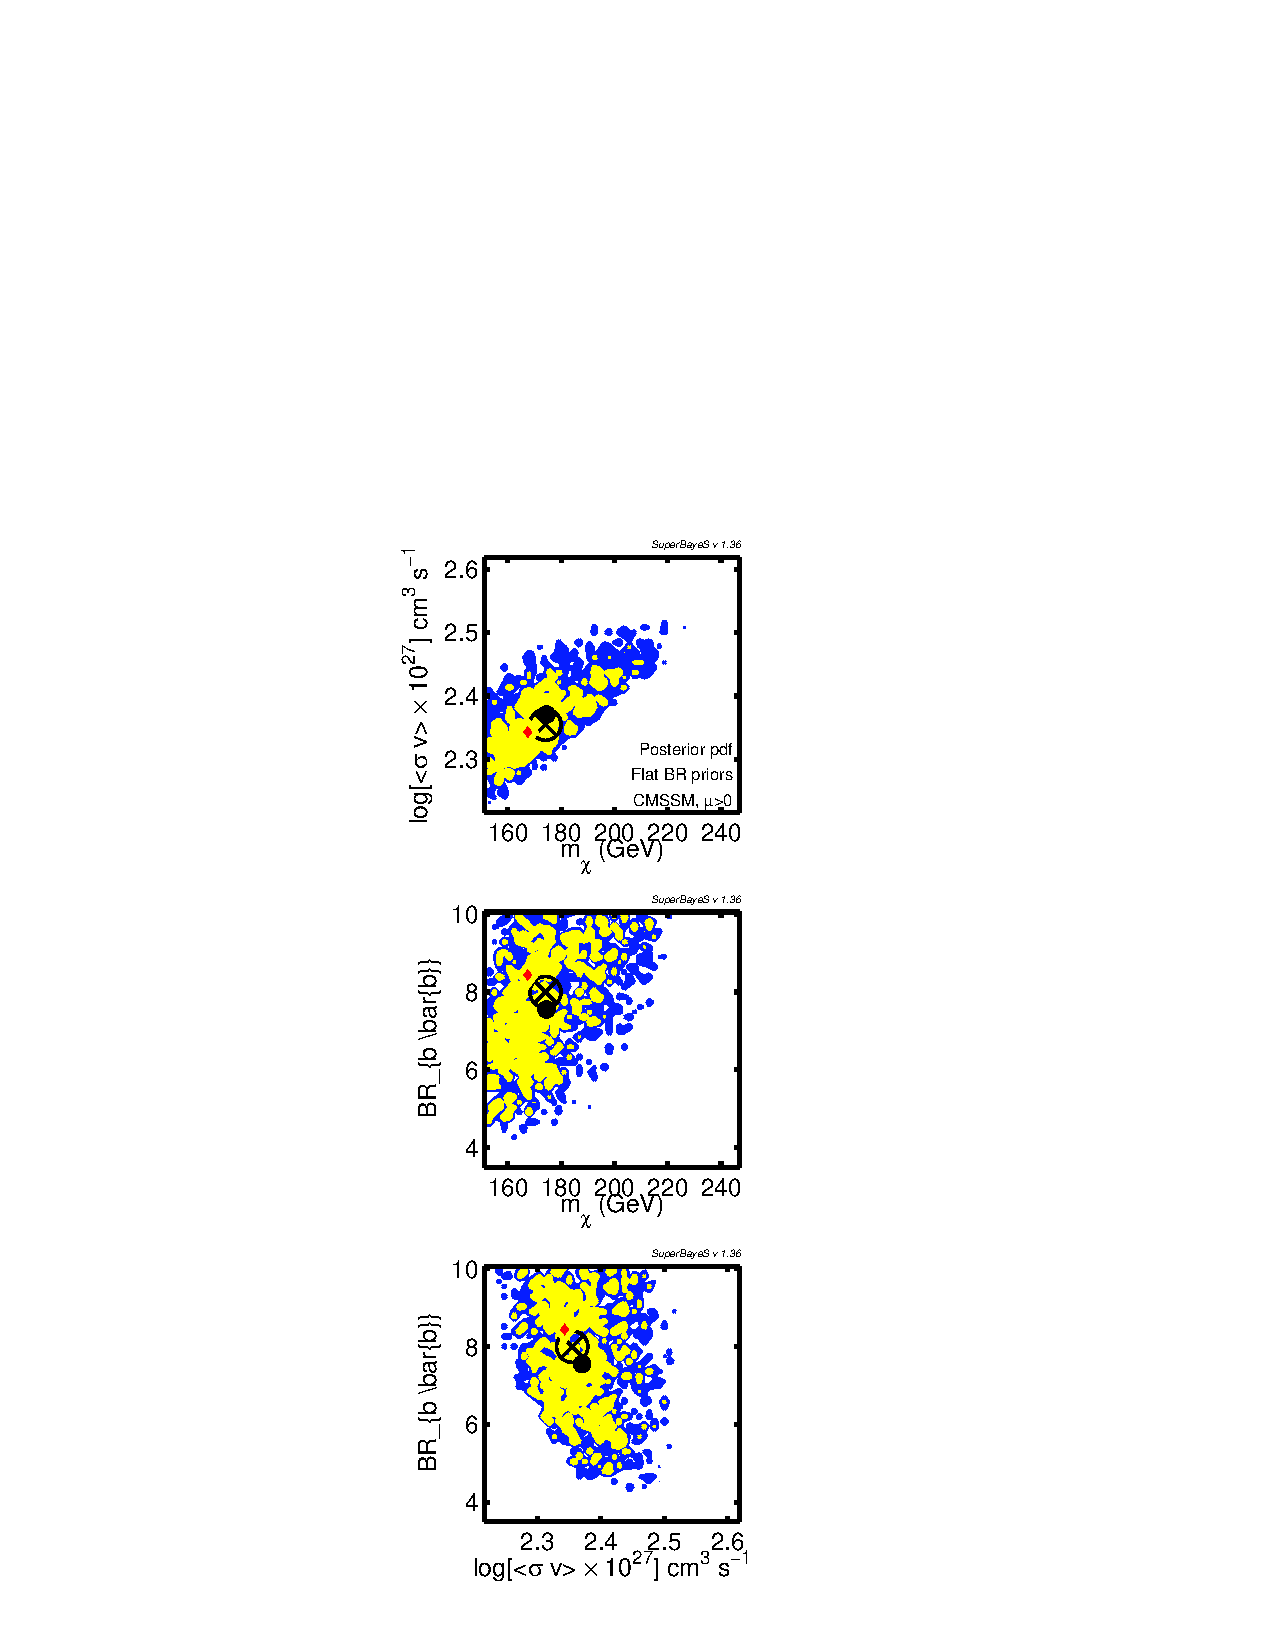
\includegraphics[trim = 190 0 200 200, clip = true, width=0.5\textwidth]{figs/F1a}
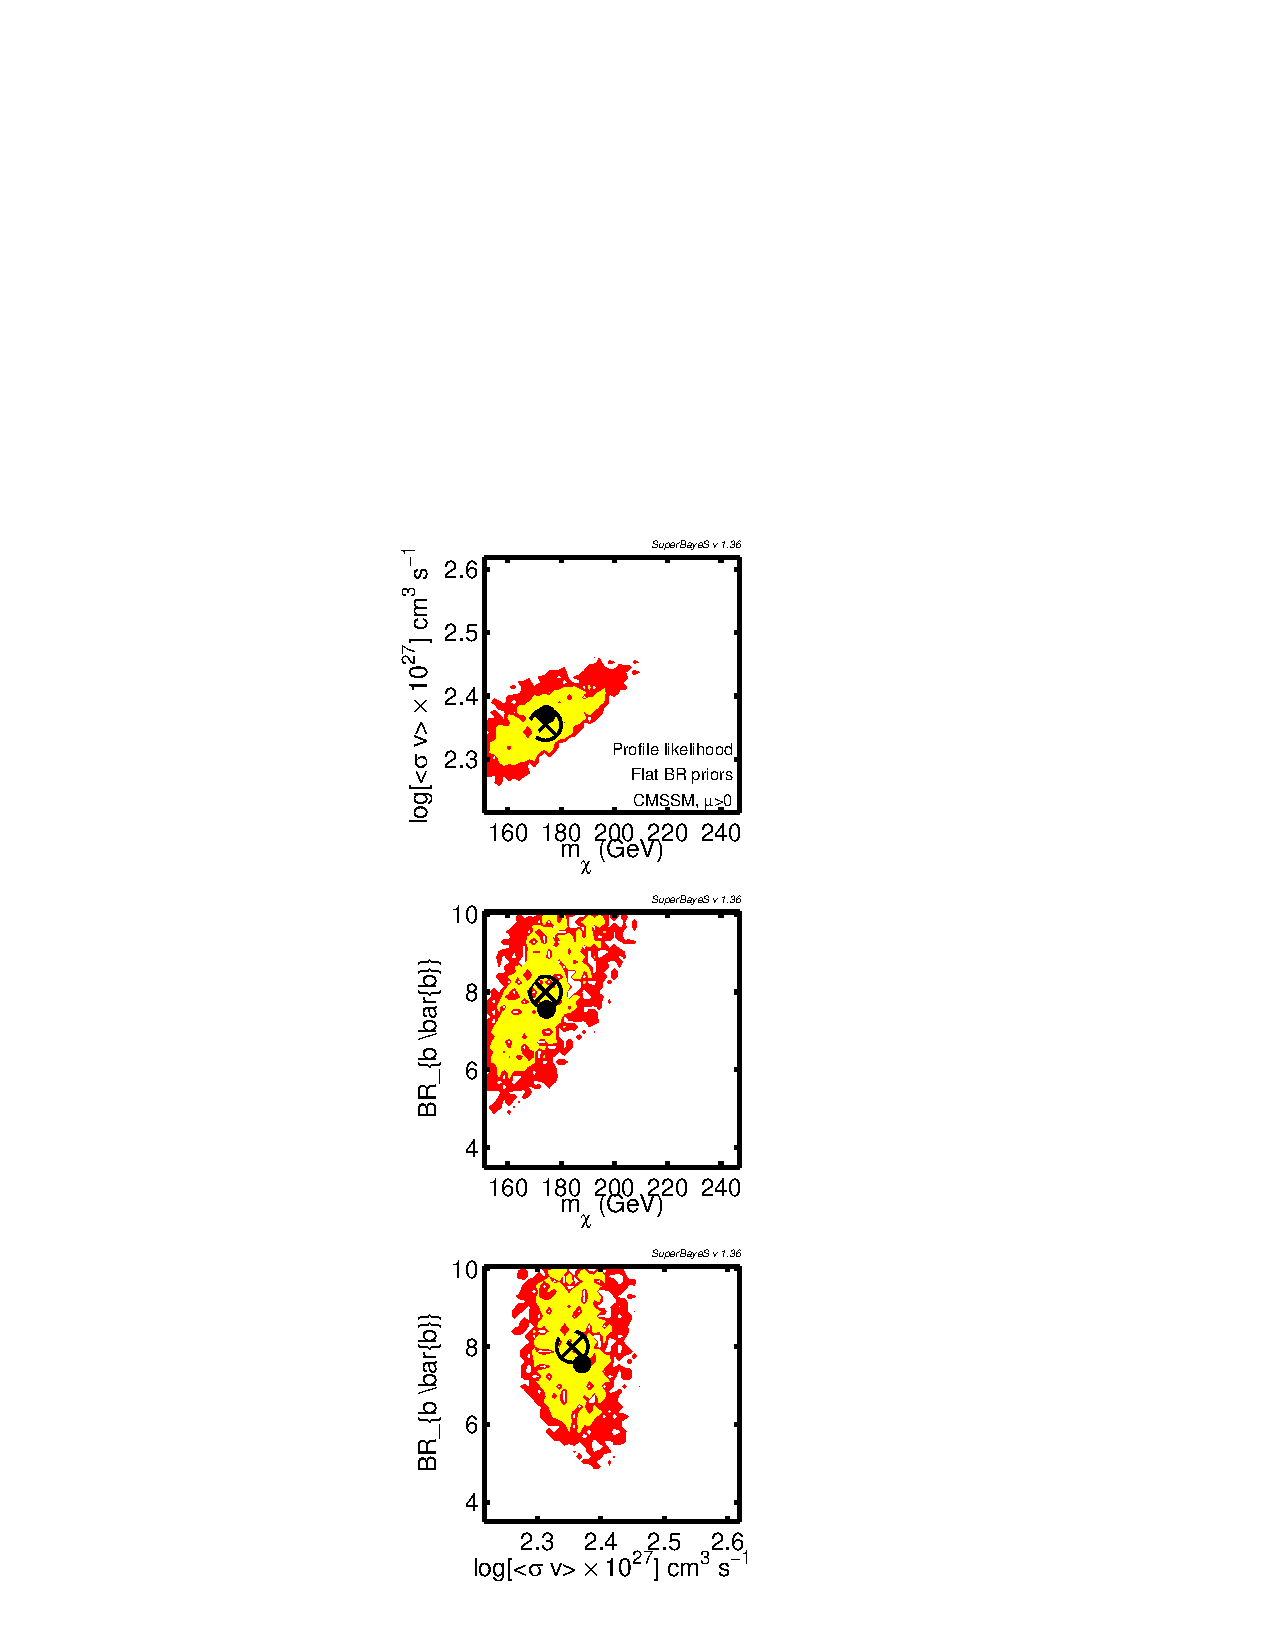
\includegraphics[trim = 190 0 200 200, clip = true, width=0.5\textwidth]{figs/F1b}
\caption{Reconstructed DM parameters using \protect\textsc{DMBayes} and \protect\textsc{flatlib}, for a simulated pure DM signal at the Galactic Centre.  The left (right) plot gives marginalised posterior PDFs (profile likelihoods), and shading indicates 1 and 2$\sigma$ credible (confidence) intervals.  Crosses indicate the best fit, bullets the posterior mean, and red/yellow diamonds the true parameter values. (Ignore annotations referring to CMSSM and \textsc{SuperBayeS})}
\label{pureDM}
\end{figure}

\begin{figure}
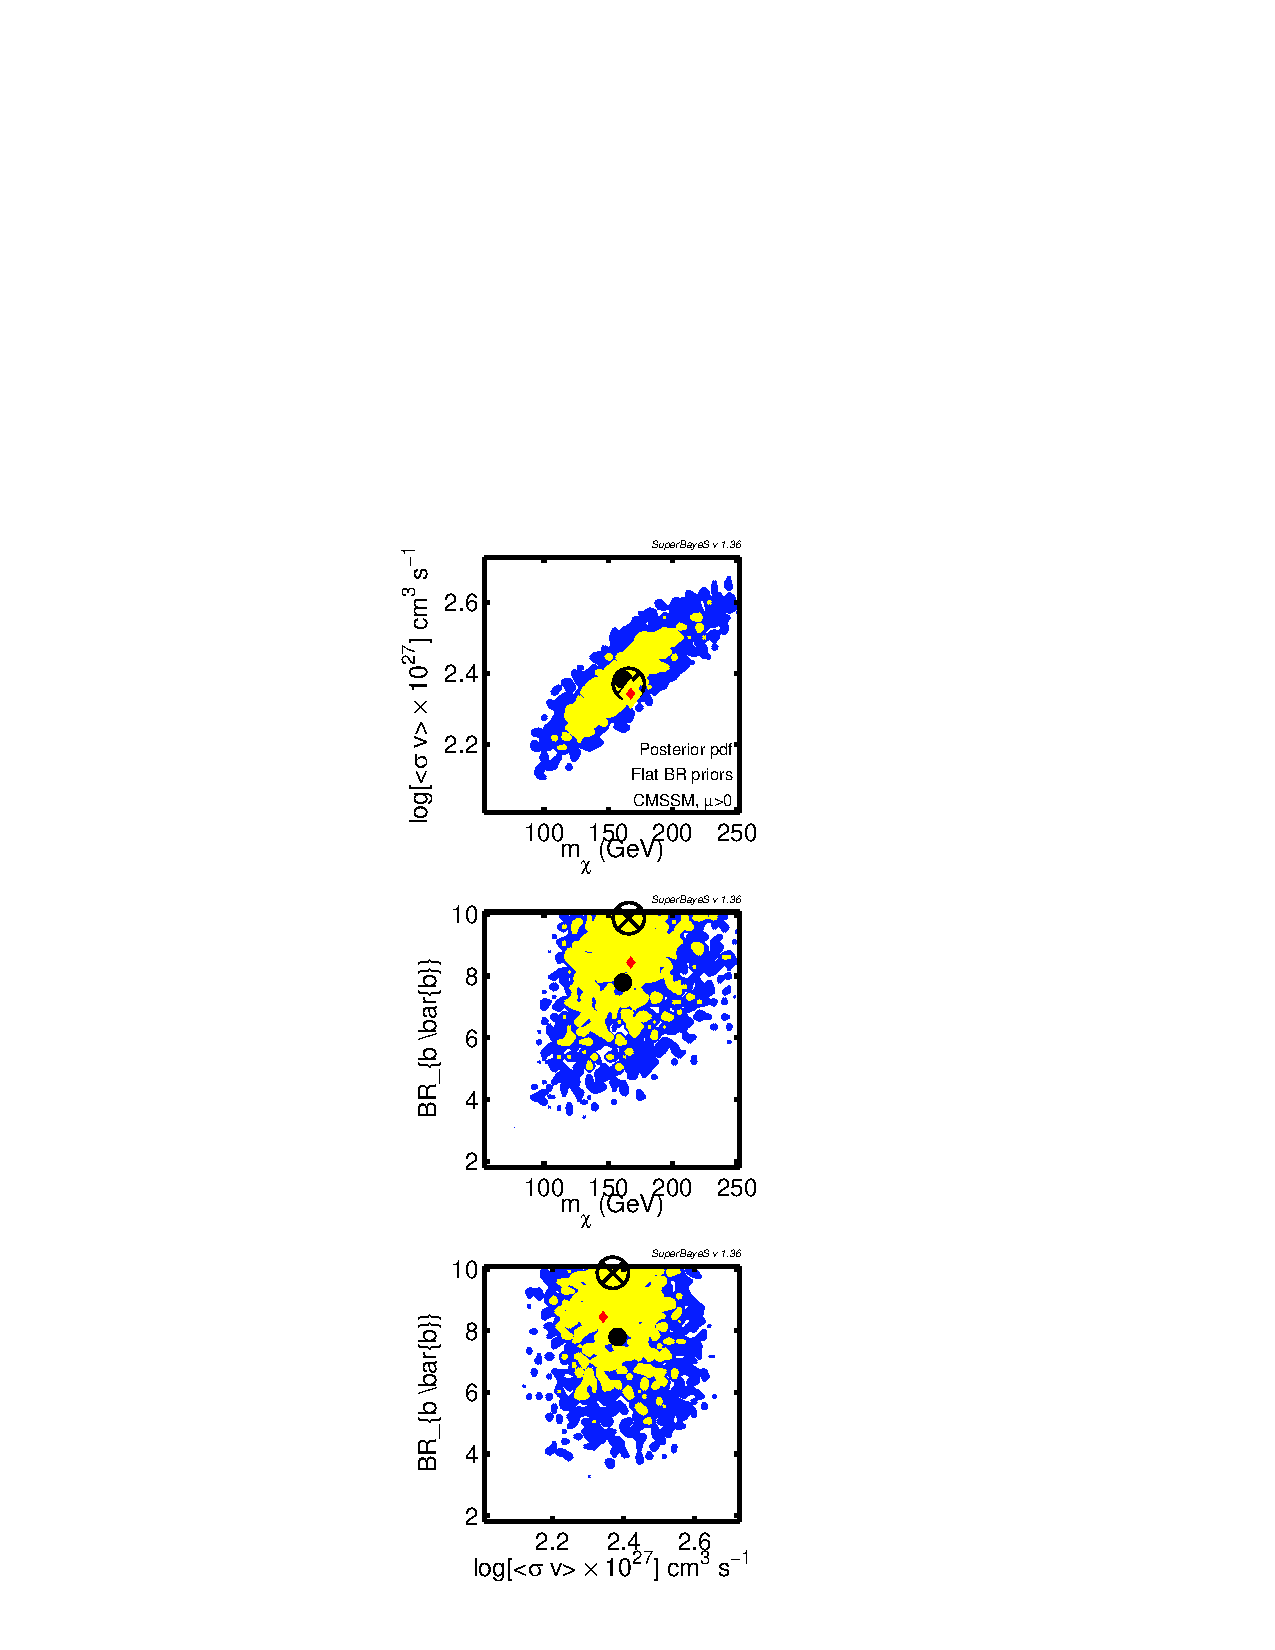
\includegraphics[trim = 190 0 200 200, clip = true, width=0.5\textwidth]{figs/F2a}
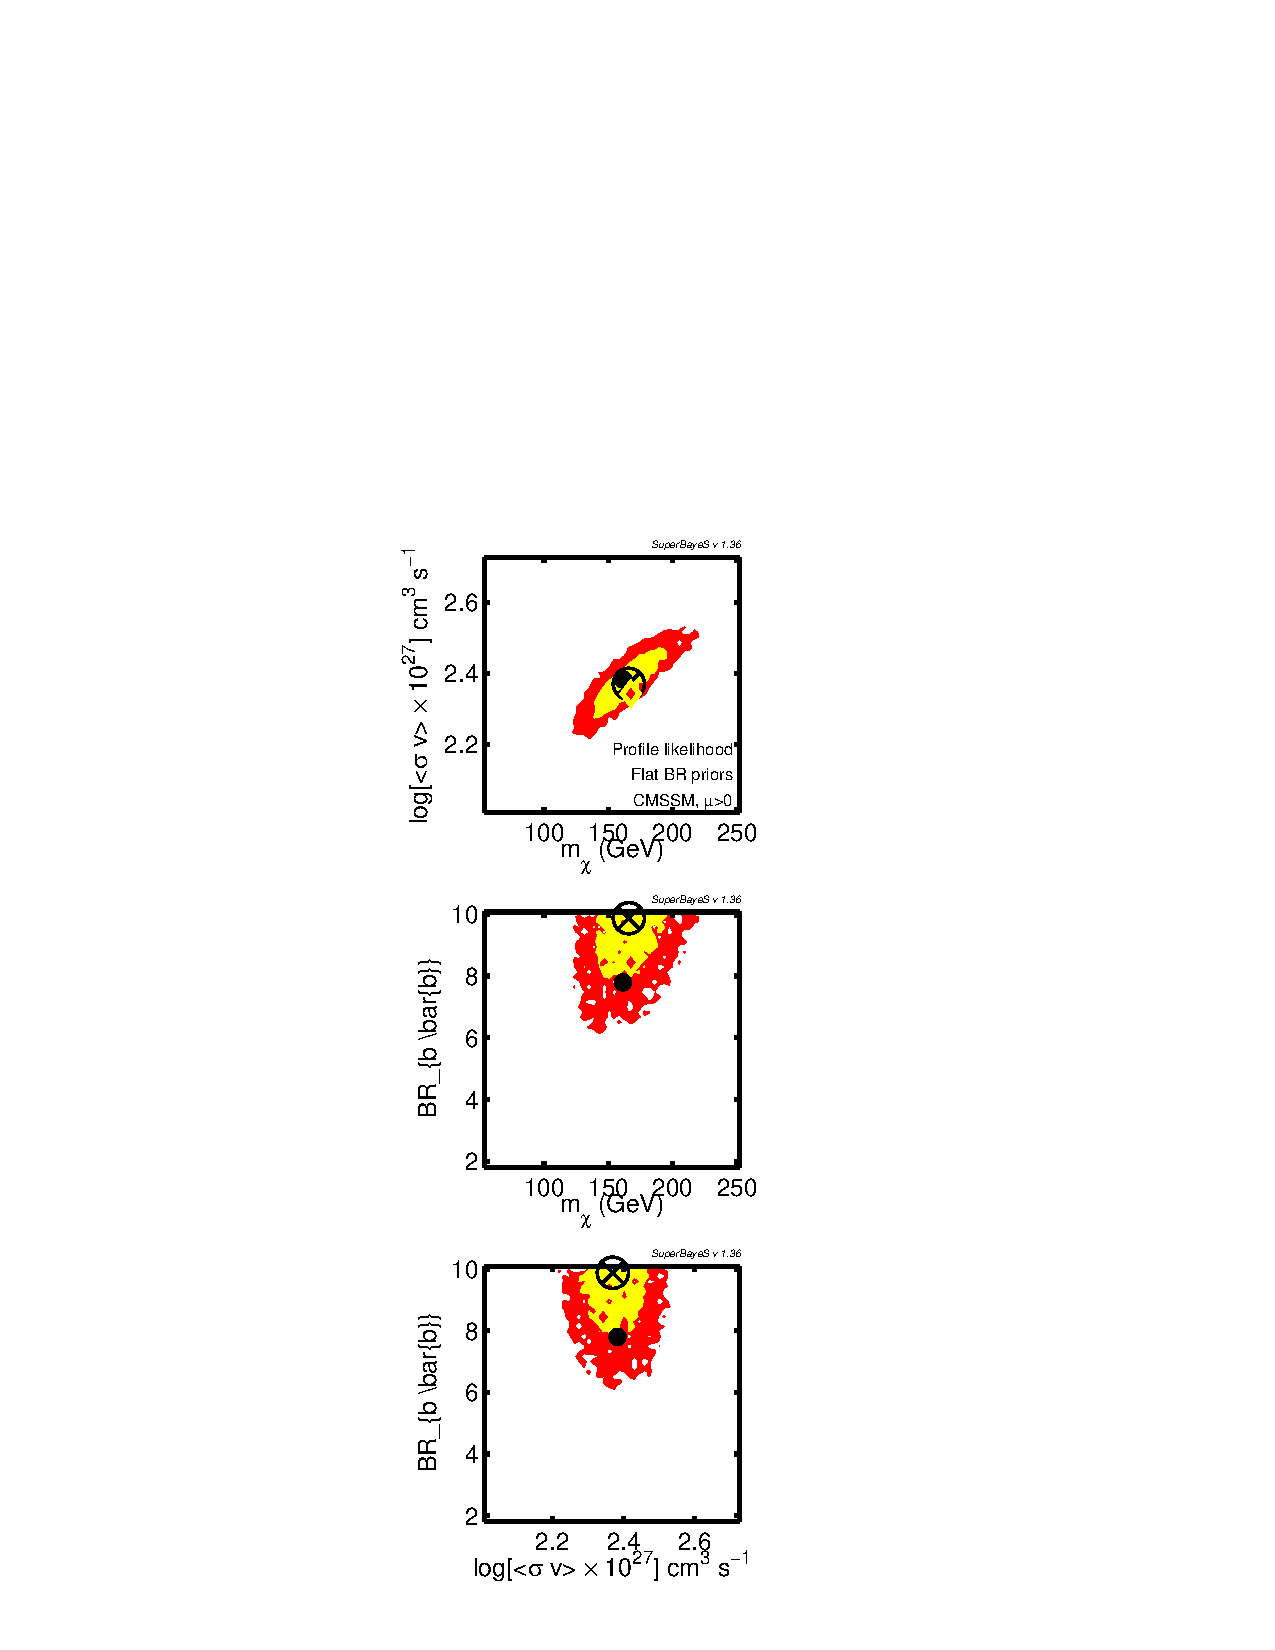
\includegraphics[trim = 190 0 200 200, clip = true, width=0.5\textwidth]{figs/F2b}
\caption{Reconstructed DM parameters using \protect\textsc{DMBayes} and \protect\textsc{flatlib} in the presence of simulated background noise (based on public Galactic and isotropic background models).  The left (right) plot gives marginalised posterior PDFs (profile likelihoods), and shading indicates 1 and 2$\sigma$ credible (confidence) intervals.  Crosses indicate the best fit, bullets the posterior mean, and red/yellow diamonds the true parameter values. (Ignore annotations referring to CMSSM and \textsc{SuperBayeS})}
\label{withBG}
\end{figure}

\section{Progress to date}

So far we have:
\begin{enumerate}
\item Developed \textsc{DMBayes}, a modified version of the \textsc{SuperBayeS} package, to perform the nested sampling+differential evolution scan over the WIMP parameter space.  \textsc{DMBayes} works with generic WIMP DM via an interface to \textsc{DMFIT}.
\item Coupled \textsc{DMBayes} to \textsc{flatlib} 
\item Written relevant likelihood and source modelling routines for the Galactic Centre
\item Implemented some rudimentary halo-marginalisation capabilities
\item Simulated a series of pure DM GC signals using \texttt{gtobssim}
\item Used these simulations to extensively test and tune DMBayes.  An example DM-only reconstruction is given in Fig.~\ref{pureDM}.
\item Added the publicly-available diffuse background models (ring and isotropic) to DMBayes as tests
\item Simulated DM GC signals with backgrounds
\item Successfully reconstructed the DM model using \textsc{DMBayes} in the presence of said backgrounds (Fig.~\ref{withBG}).
\item Resolved a large number of technical and architecture-specific instabilities encountered when running early versions of DMBayes.
\item Upgraded \textsc{flatlib} to work with Pass 7 IRFs
\item Implemented the treatment of the diffuse BG and tested it in BG only simulations
\item Coupled \textsc{DMBayeS} to \textsc{Diver}, a forthcoming differential evolution package from Roebber \& Scott
\item Developed, implemented and tested the point source identification strategy
\end{enumerate}

\section{Internal history within the Fermi Collaboration}

This analysis was proposed in October 2009, and an external author request for some of the involved parties approved (Roberto Trotta \& Roberto Ruiz de Austri).  Other external authors initially approved (Cumberbatch \& Roszkowski) did not ultimately become involved.  Pat's present status within the Collaboration is somewhat grey, so he may or may not require approval as an external author at a later stage.

Since October 2009, progress has been incremental but steady, with a small number of contributors extensively developing and testing the tools as time permitted.  In mid 2010 the analysis reached a sufficiently mature stage for further development to be concretely discussed and carried out with others in the Collaboration; discussions and collaborative efforts began at this point with members of the Diffuse/Galprop group, leading to Gulli et al's involvement.

\section{Some notes on specific parts of the code/analysis}

\subsection{Inference for general BR setup}

As a first step a prior for the branching ratios had to be found. Instead of choosing a prior directly on the branching ratios it was decided to implement a log prior on the annihilation cross-sections. The branching ratios can be calculated from the cross-sections as
\begin{equation}
BR_{\chi\chi \rightarrow r_i r_i} = \frac{\sigma_{\chi\chi \rightarrow r_i r_i}}{\sum_j \sigma_{\chi\chi \rightarrow r_j r_j}}
\end{equation}
The resulting effective prior on the branching ratios ensures that they add up to one. \\

The shape of this effective prior depends strongly on the prior range chosen for the log prior on the cross-sections. Three examples for the shape of the prior on the branching ratios in eight dimensions (i.e.\ for eight open annihilation channels) are shown in Fig.~\ref{BRPriorShape}. From left to right the plots correspond to a log prior range for the cross-sections of 1, 4 and 10. As can be seen, due to the high dimensionality small values of the BR are strongly favoured for the two larger ranges. This trend becomes less extreme when the number of open annihilation channels is reduced. \\

\begin{figure}
\centering
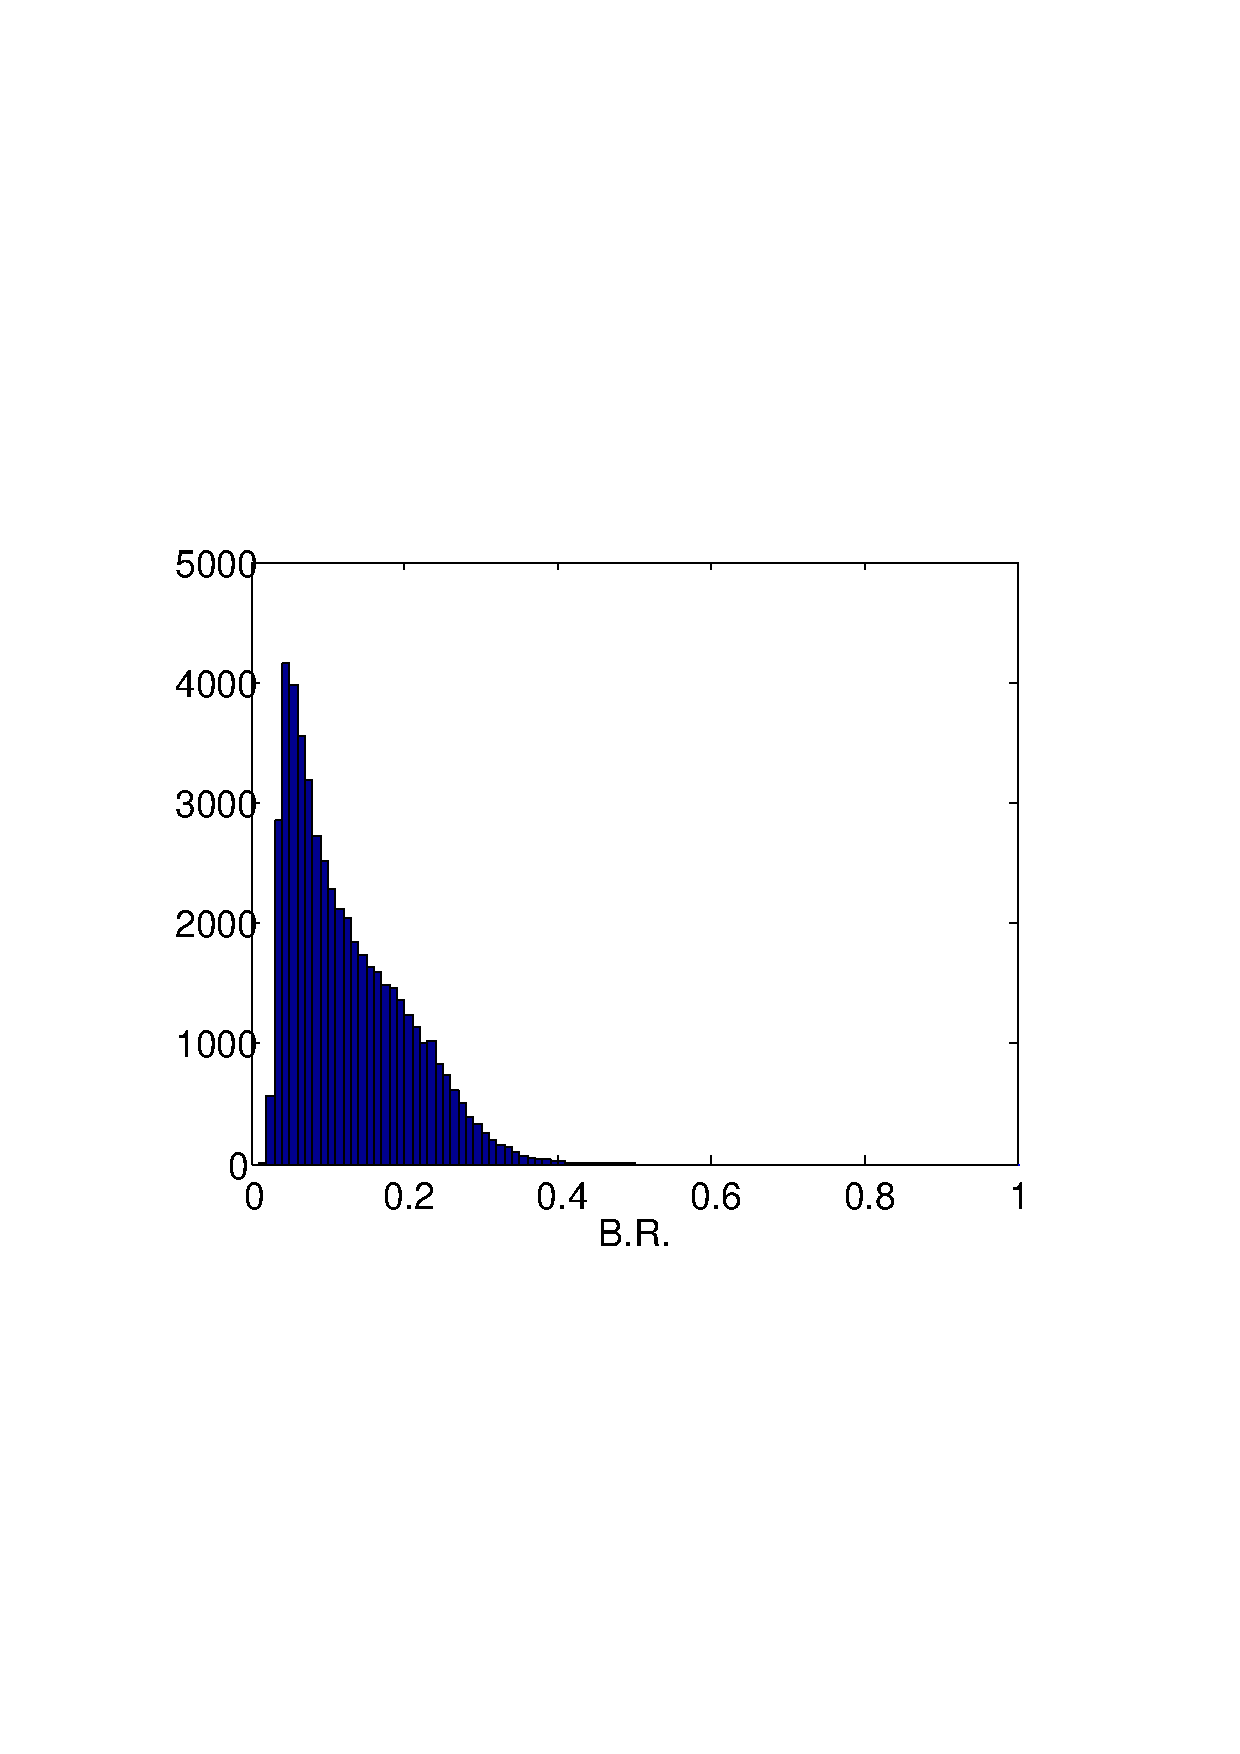
\includegraphics[trim = 70 230 100 230, clip = true, width=0.32\textwidth]{figs/BR_Prior_CS_Range1}
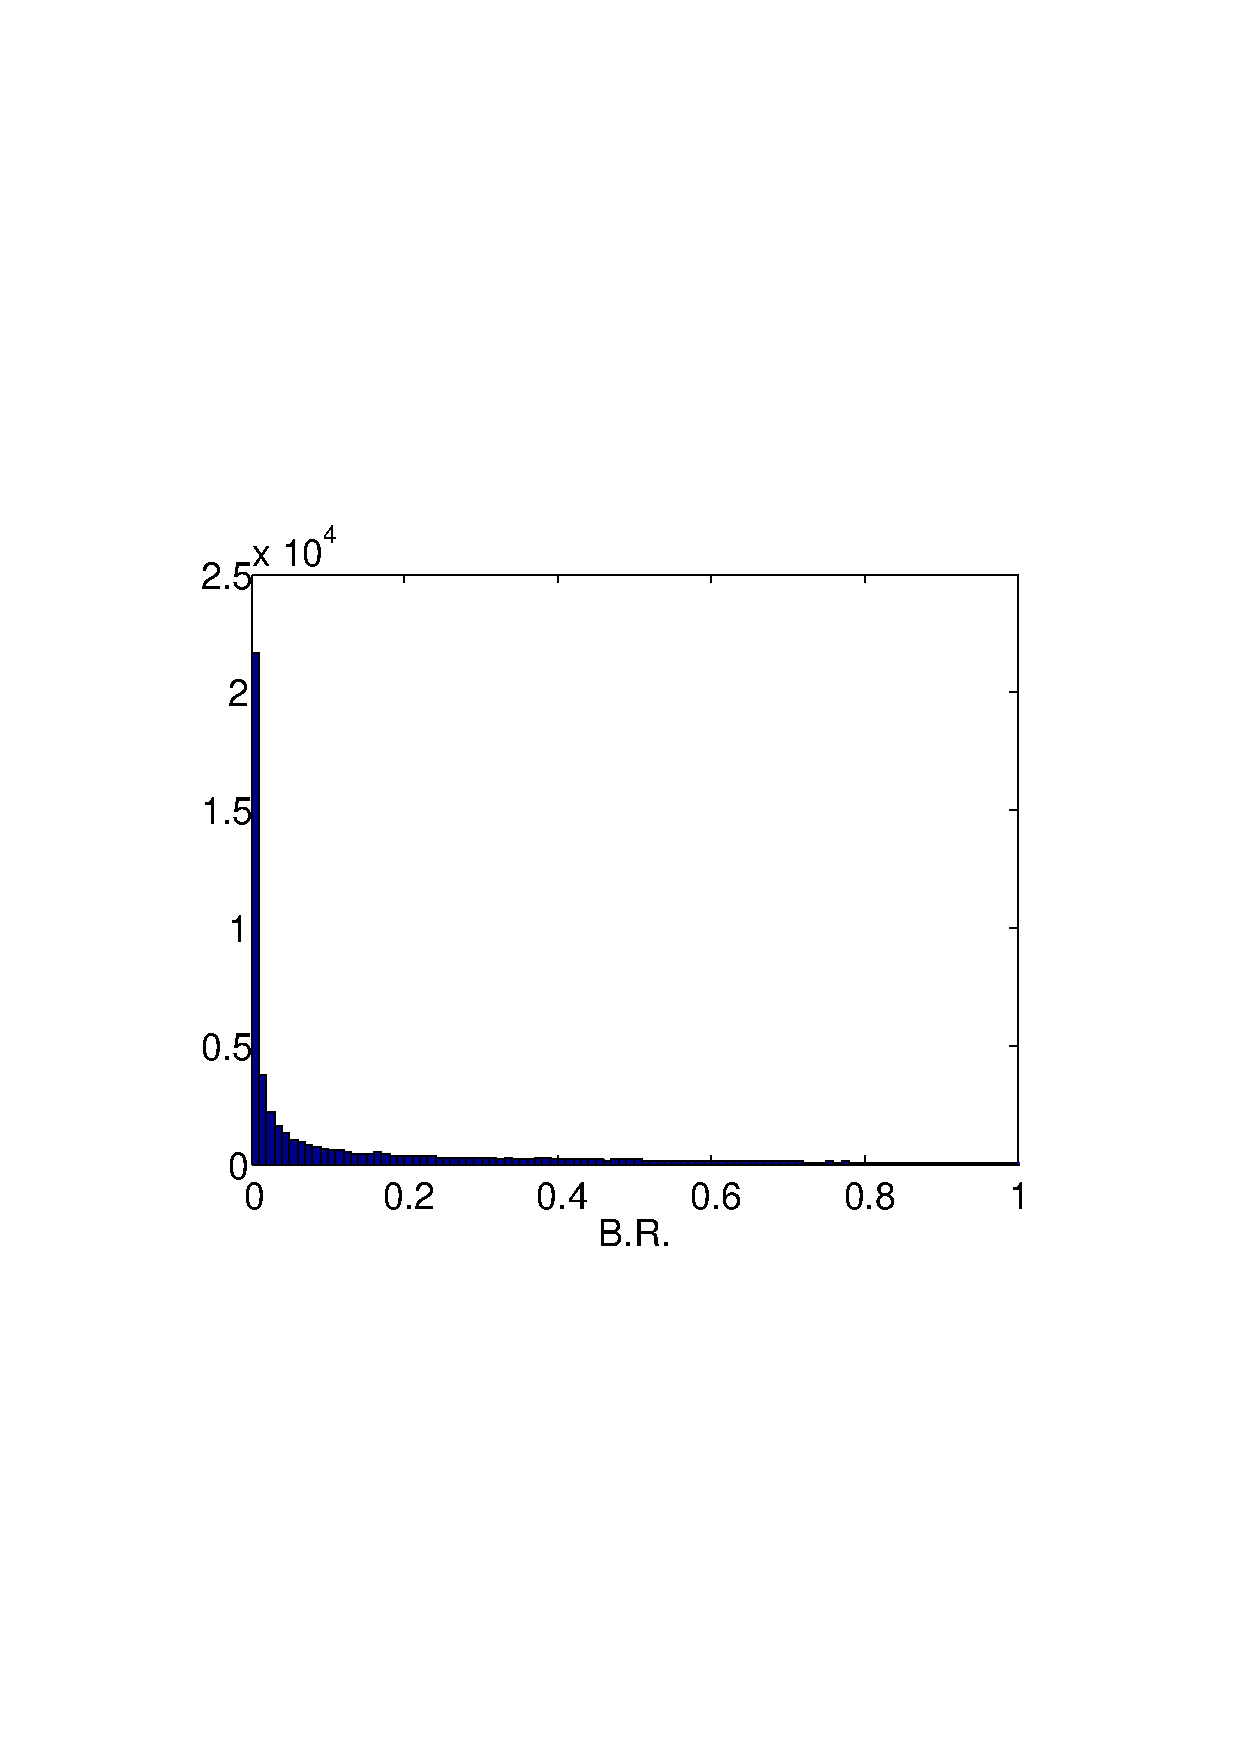
\includegraphics[trim = 80 230 100 230, clip = true, width=0.32\textwidth]{figs/BR_Prior_CS_Range4}
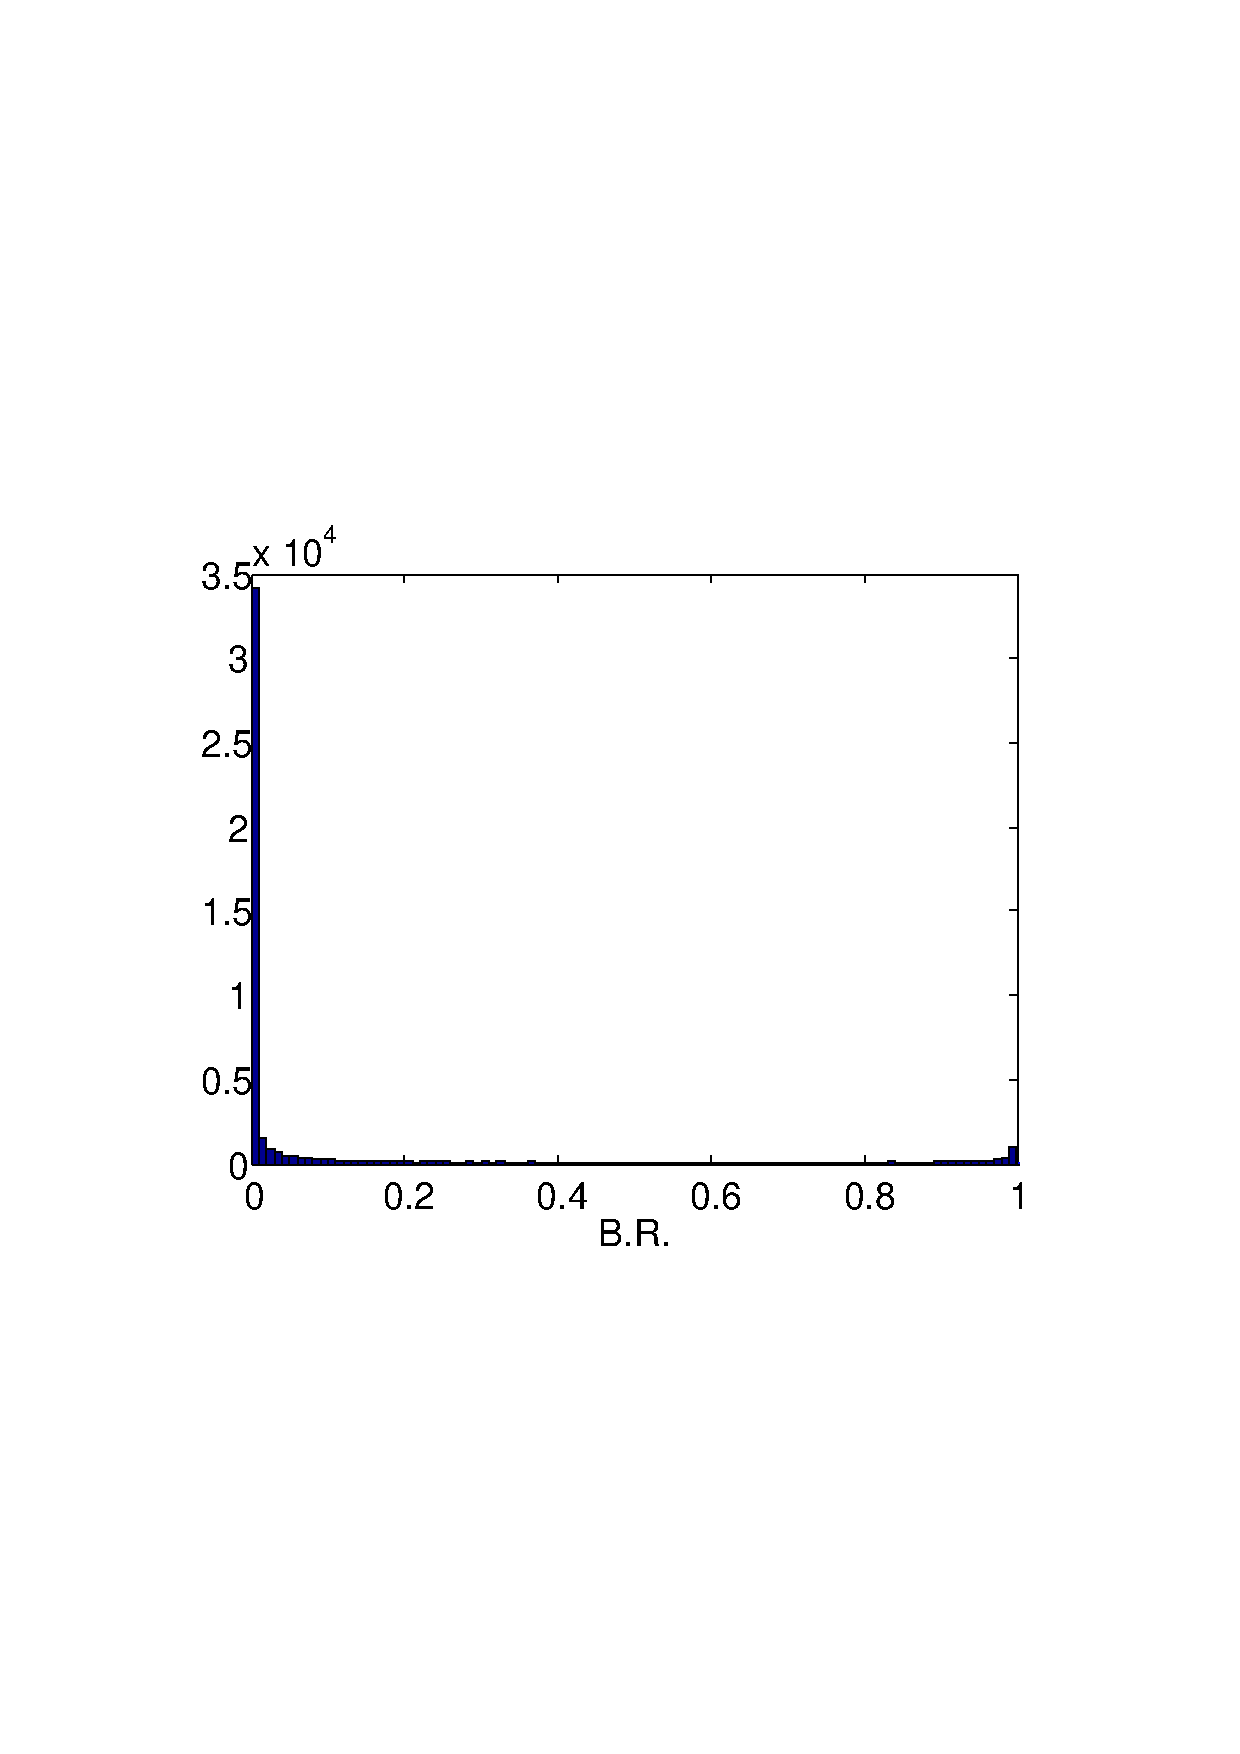
\includegraphics[trim = 80 230 100 230, clip = true, width=0.32\textwidth]{figs/BR_Prior_CS_Range10}
\caption{Shape of the effective prior on the branching ratios as a function of the range of the log prior on the cross-sections in eight dimensions. From top to bottom the range is equal to 1, 4 and 10.}
\label{BRPriorShape}
\end{figure}

To investigate the influence of this choice of prior on the posterior distribution a scan of the parameter space was carried out assuming nine open annihilation channels, and imposing a log prior on the cross-sections with range $[-2.0,3.5]$. A range of 5.5 was chosen, because for this range intermediate and high values of the BRs are equally well sampled by the prior. The true point is given by $m_{\chi} = 167$\ GeV, $\textnormal{log}(<\sigma v> \cdot 10^{+27} \textnormal{cm}^3 \textnormal{s}^{-1}) = 2.34$, $BR_{b \bar{b}} = 0.844$, $BR_{\tau^+ \tau^-} = 0.156$, $BR(\textnormal{others}) \approx 0$. The simulated data include background noise, based on public Galactic and isotropic background models. A scan with Bayesian set-up (Nested Sampling parameters nlive = 2000, tol = 0.5, eff = 0.3) was carried out to reconstruct the DM parameters.
The resulting plots of the profile likelihood and the marginalised posterior distribution are shown in Fig. \ref{Bayesianscan}. 
\begin{figure}
\centering
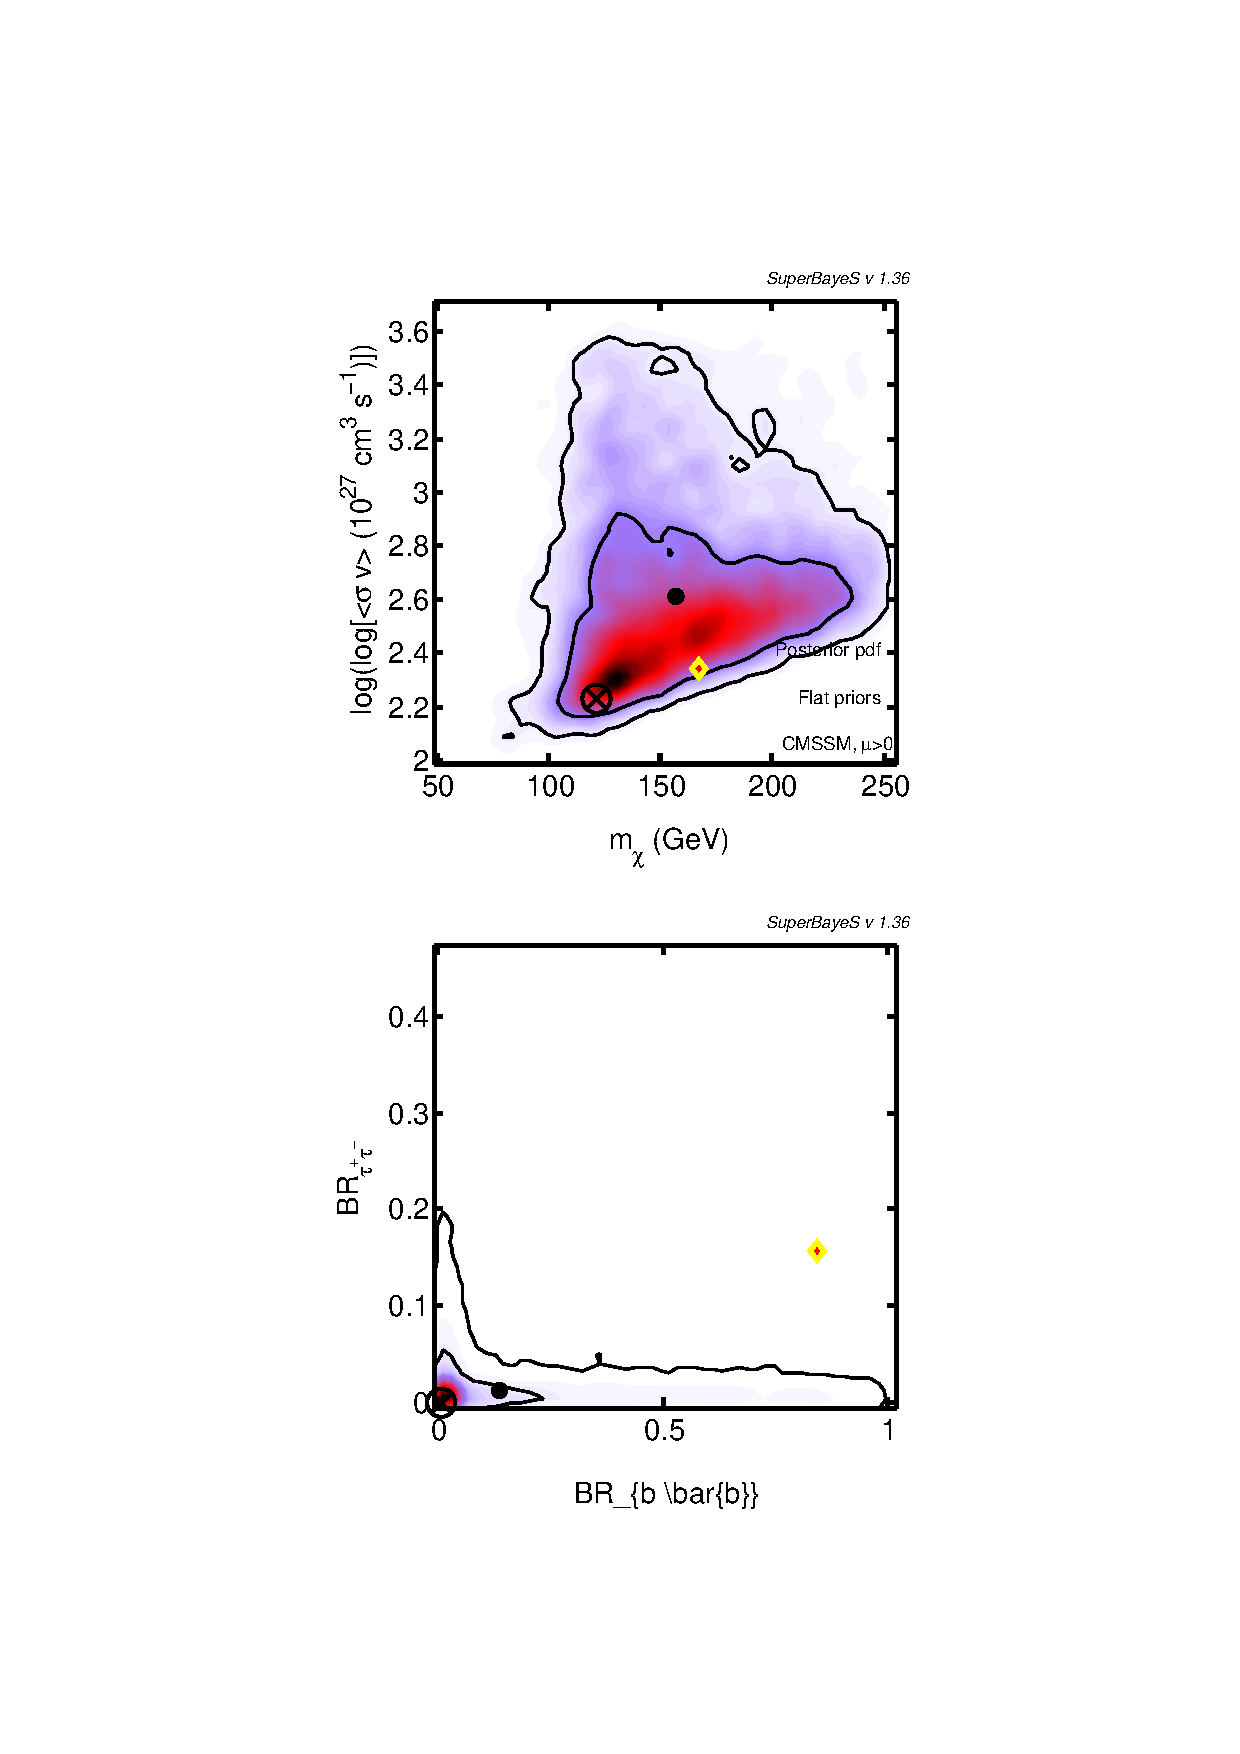
\includegraphics[trim = 140 120 140 120, clip = true, width=0.46\textwidth]{figs/2D_Posterior}
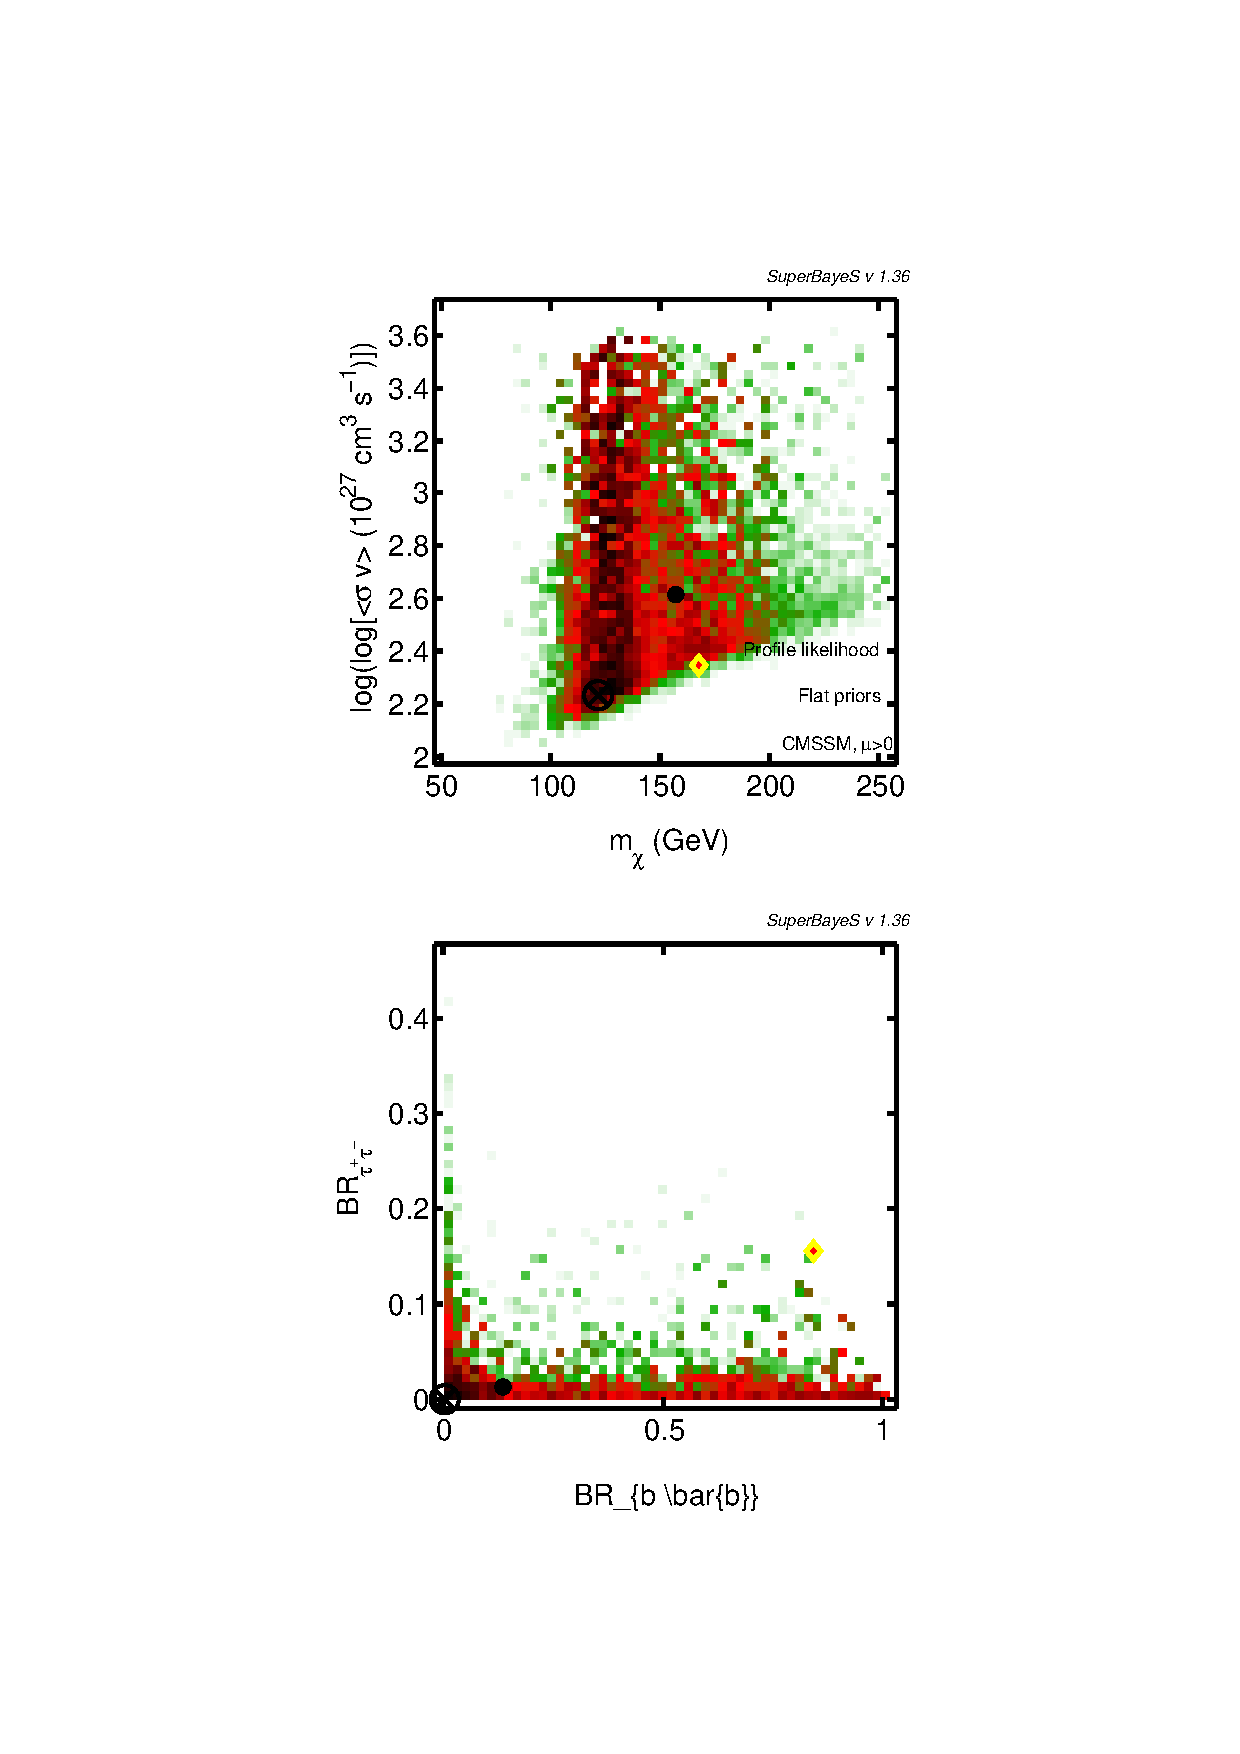
\includegraphics[trim = 140 120 140 120, clip = true, width=0.46\textwidth]{figs/2D_PL}
\caption{Parameter inference results from a scan with Bayesian set-up. The left (right) plots give marginalised posterior PDFs (profile likelihoods).  Crosses indicate the best fit, bullets the posterior mean, and red/yellow diamonds the true parameter values. (Ignore annotations referring to CMSSM and \textsc{SuperBayeS})}
\label{Bayesianscan}
\end{figure}
The WIMP mass and annihilation cross-section are reasonably well reconstructed, the true point is contained within the 2D $68\%$ credible interval. However, the marginalised posterior distribution for the BRs is centred at very low values, far away from the true point. Likewise, the best fit point is also quite far away from the true point. \\
\begin{figure}
\centering
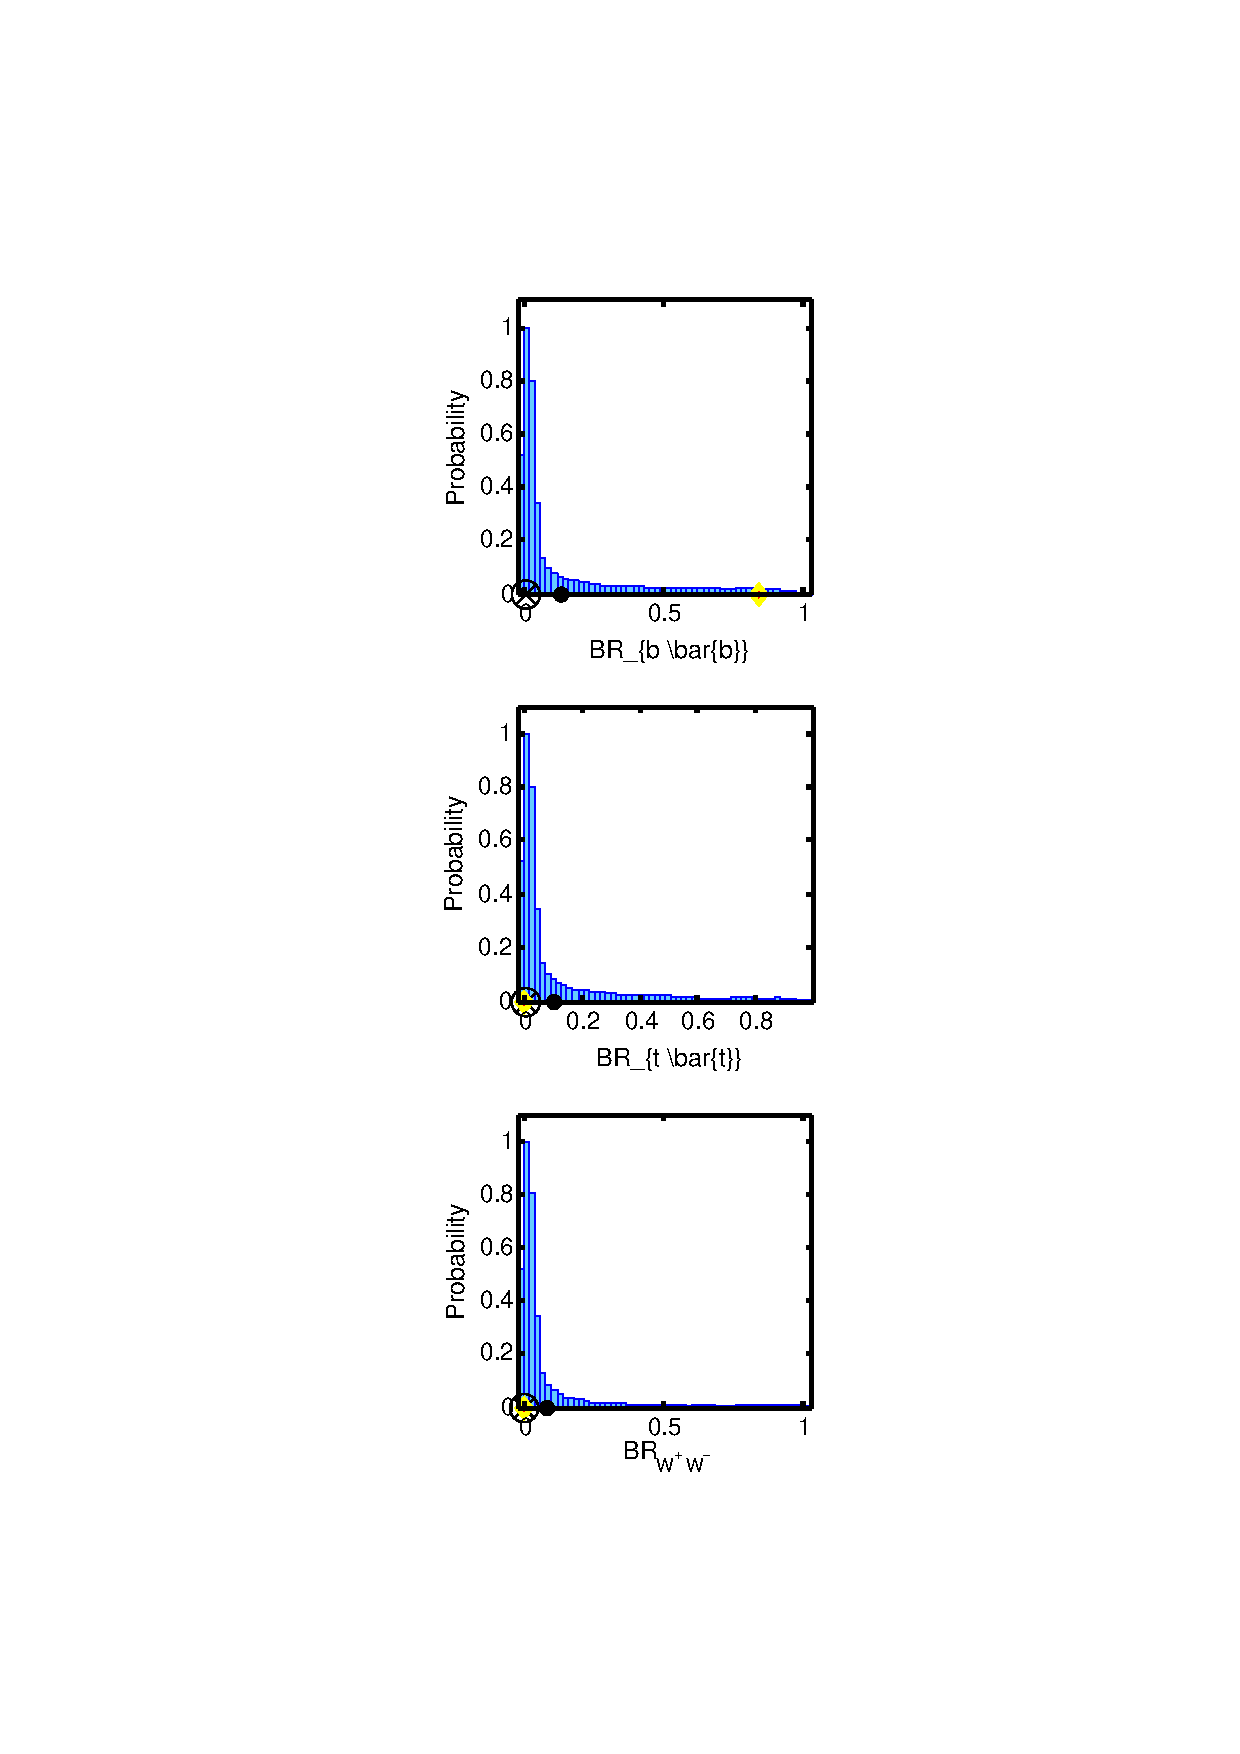
\includegraphics[trim = 205 100 202 100, clip = true, width=0.32\textwidth]{figs/1D_Posterior_BR_1}
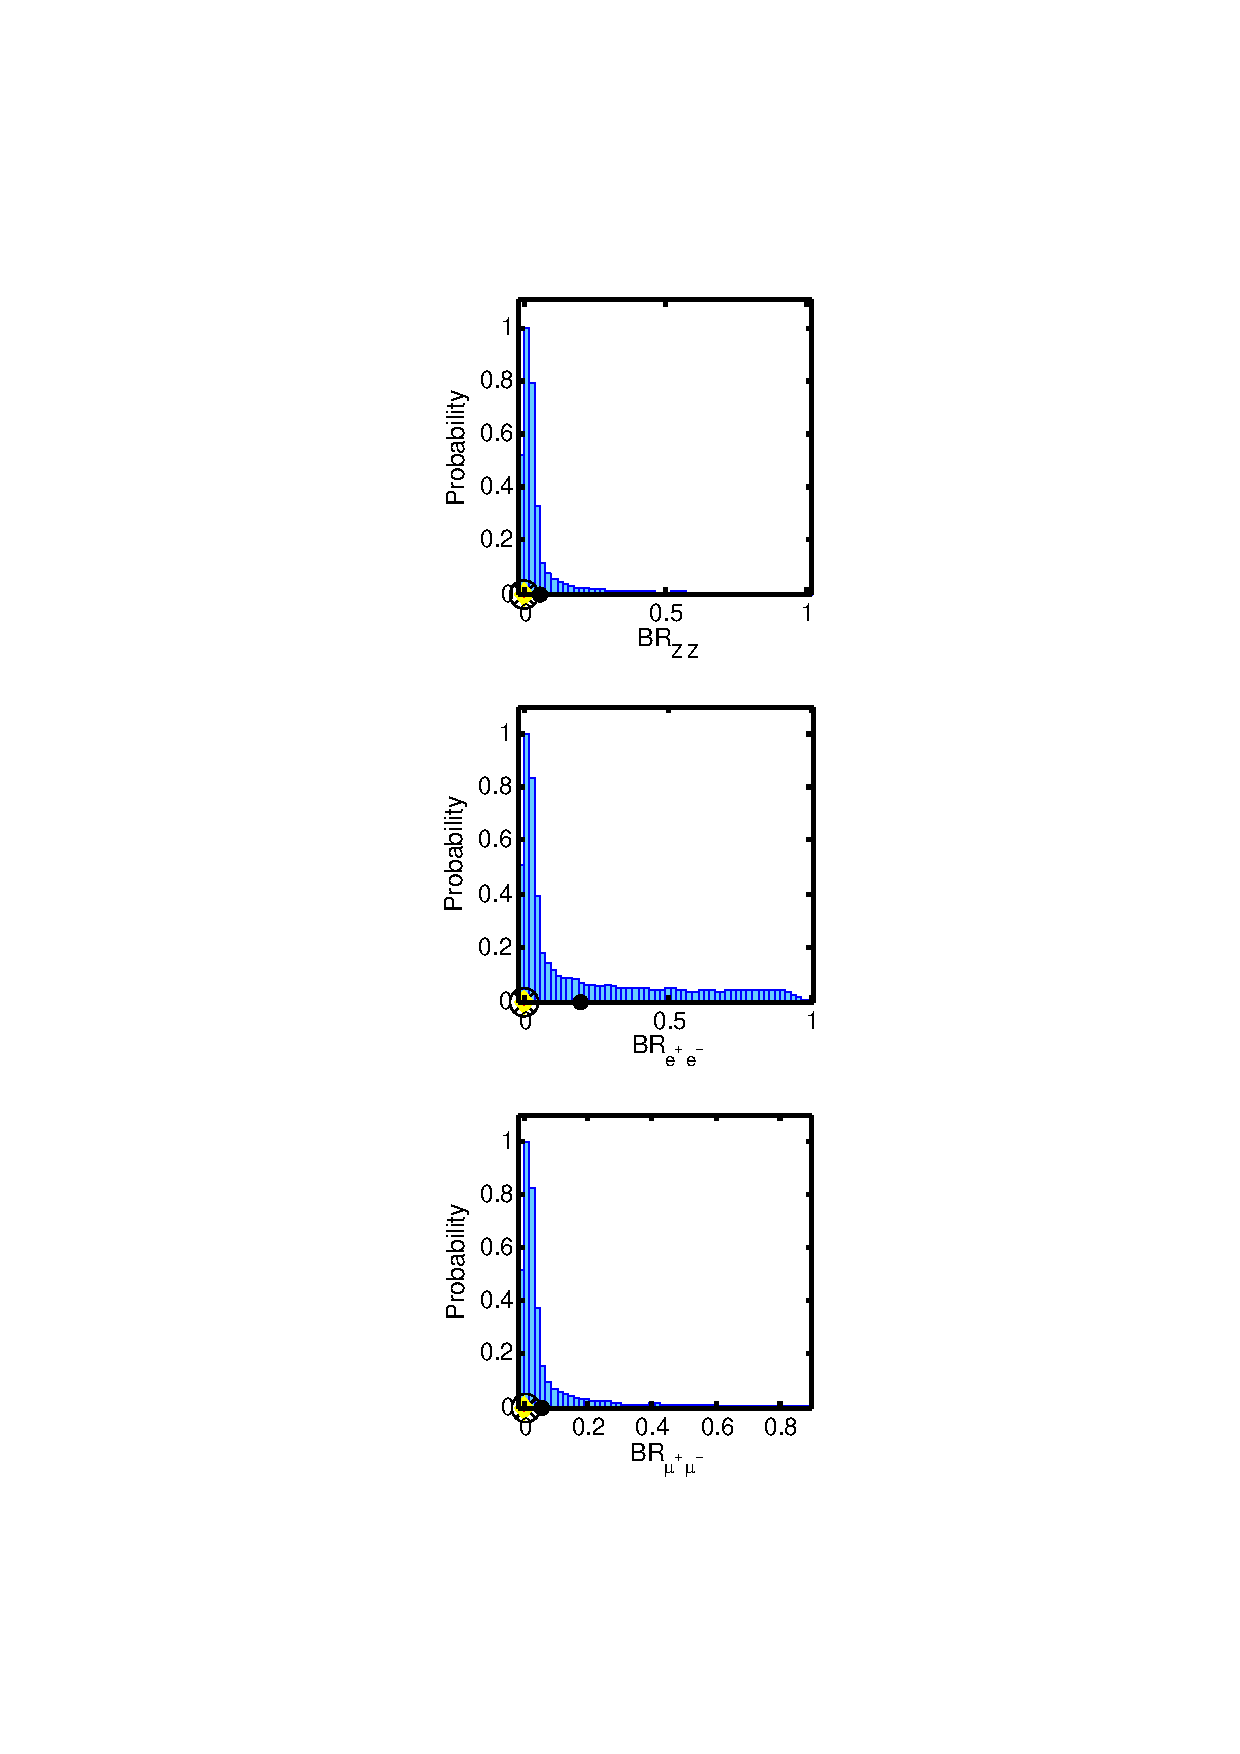
\includegraphics[trim = 205 100 202 100, clip = true, width=0.32\textwidth]{figs/1D_Posterior_BR_2}
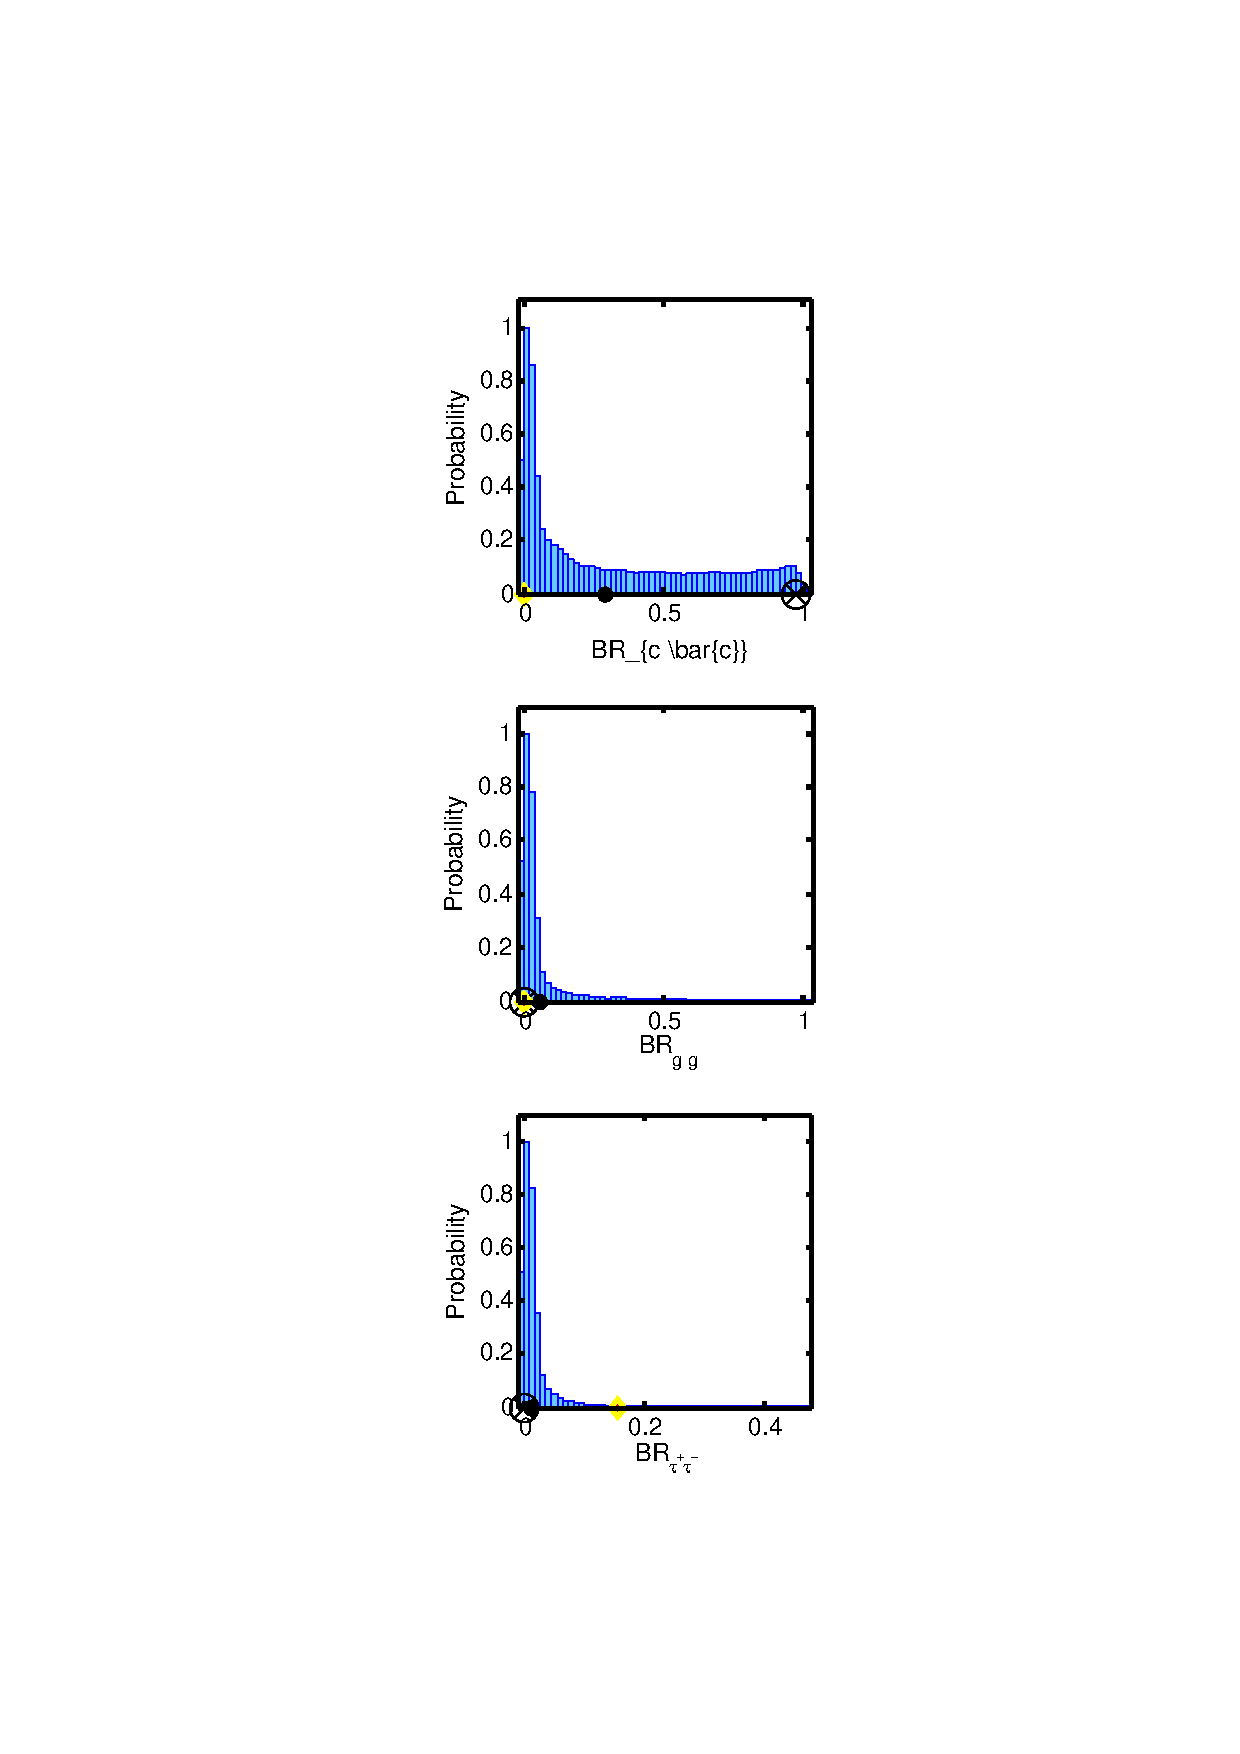
\includegraphics[trim = 205 100 202 100, clip = true, width=0.32\textwidth]{figs/1D_Posterior_BR_3}
\caption{1D marginalised posterior PDFs of the BRs resulting from a scan with Bayesian set-up. Crosses indicate the best fit, bullets the posterior mean, and red/yellow diamonds the true parameter values. (Ignore annotations referring to CMSSM and \textsc{SuperBayeS})}
\label{1DpostBR}
\end{figure}

From the 1D posterior PDFs of the BRs (see Fig. \ref{1DpostBR}) one can see that the posterior is strongly prior dominated: the shape of the 1D posteriors strongly resembles the shape of the prior distributions. Clearly the available data is not strong enough to overcome the impact of the prior. It can be concluded that while the posterior PDF can provide some information about the underlying parameter space, in most cases the impact of the prior will be too strong to allow for reliable parameter inference using the posterior PDF. Better results could be obtained from the profile likelihood distribution. For the Bayesian scan, the profile likelihood is not well-sampled around the true point, as can be seen from the 2D profile likelihood plots. In order to obtain reliable results form the profile likelihood, the above scan was repeated for a PL set-up (MultiNest parameters nlive = 20000, tol = 0.0001, eff = 0.3). The resulting plots of the 2D posterior PDFs and profile likelihoods are given in Fig. \ref{PLscan}. \\

\begin{figure}
\centering
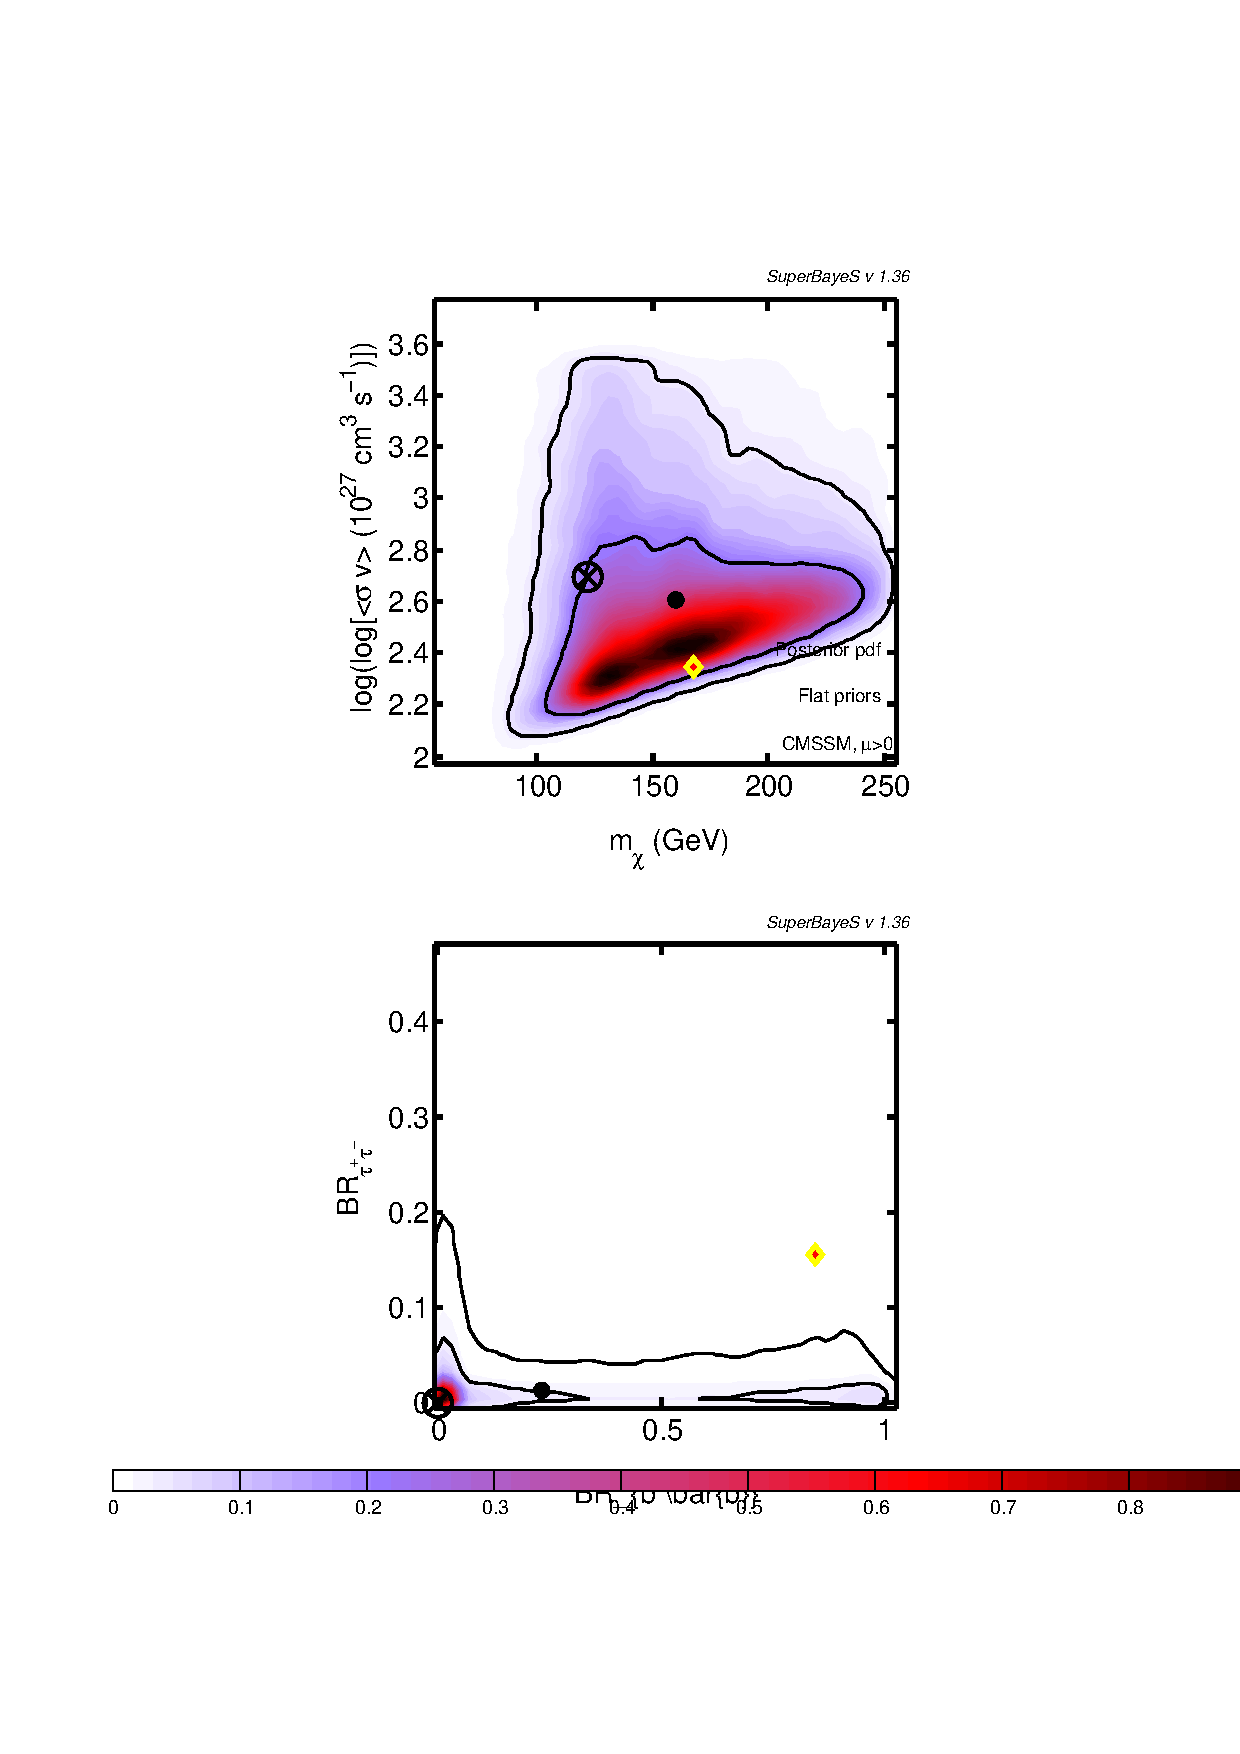
\includegraphics[trim = 140 120 140 120, clip = true, width=0.46\textwidth]{figs/2D_Posterior_PLscan}
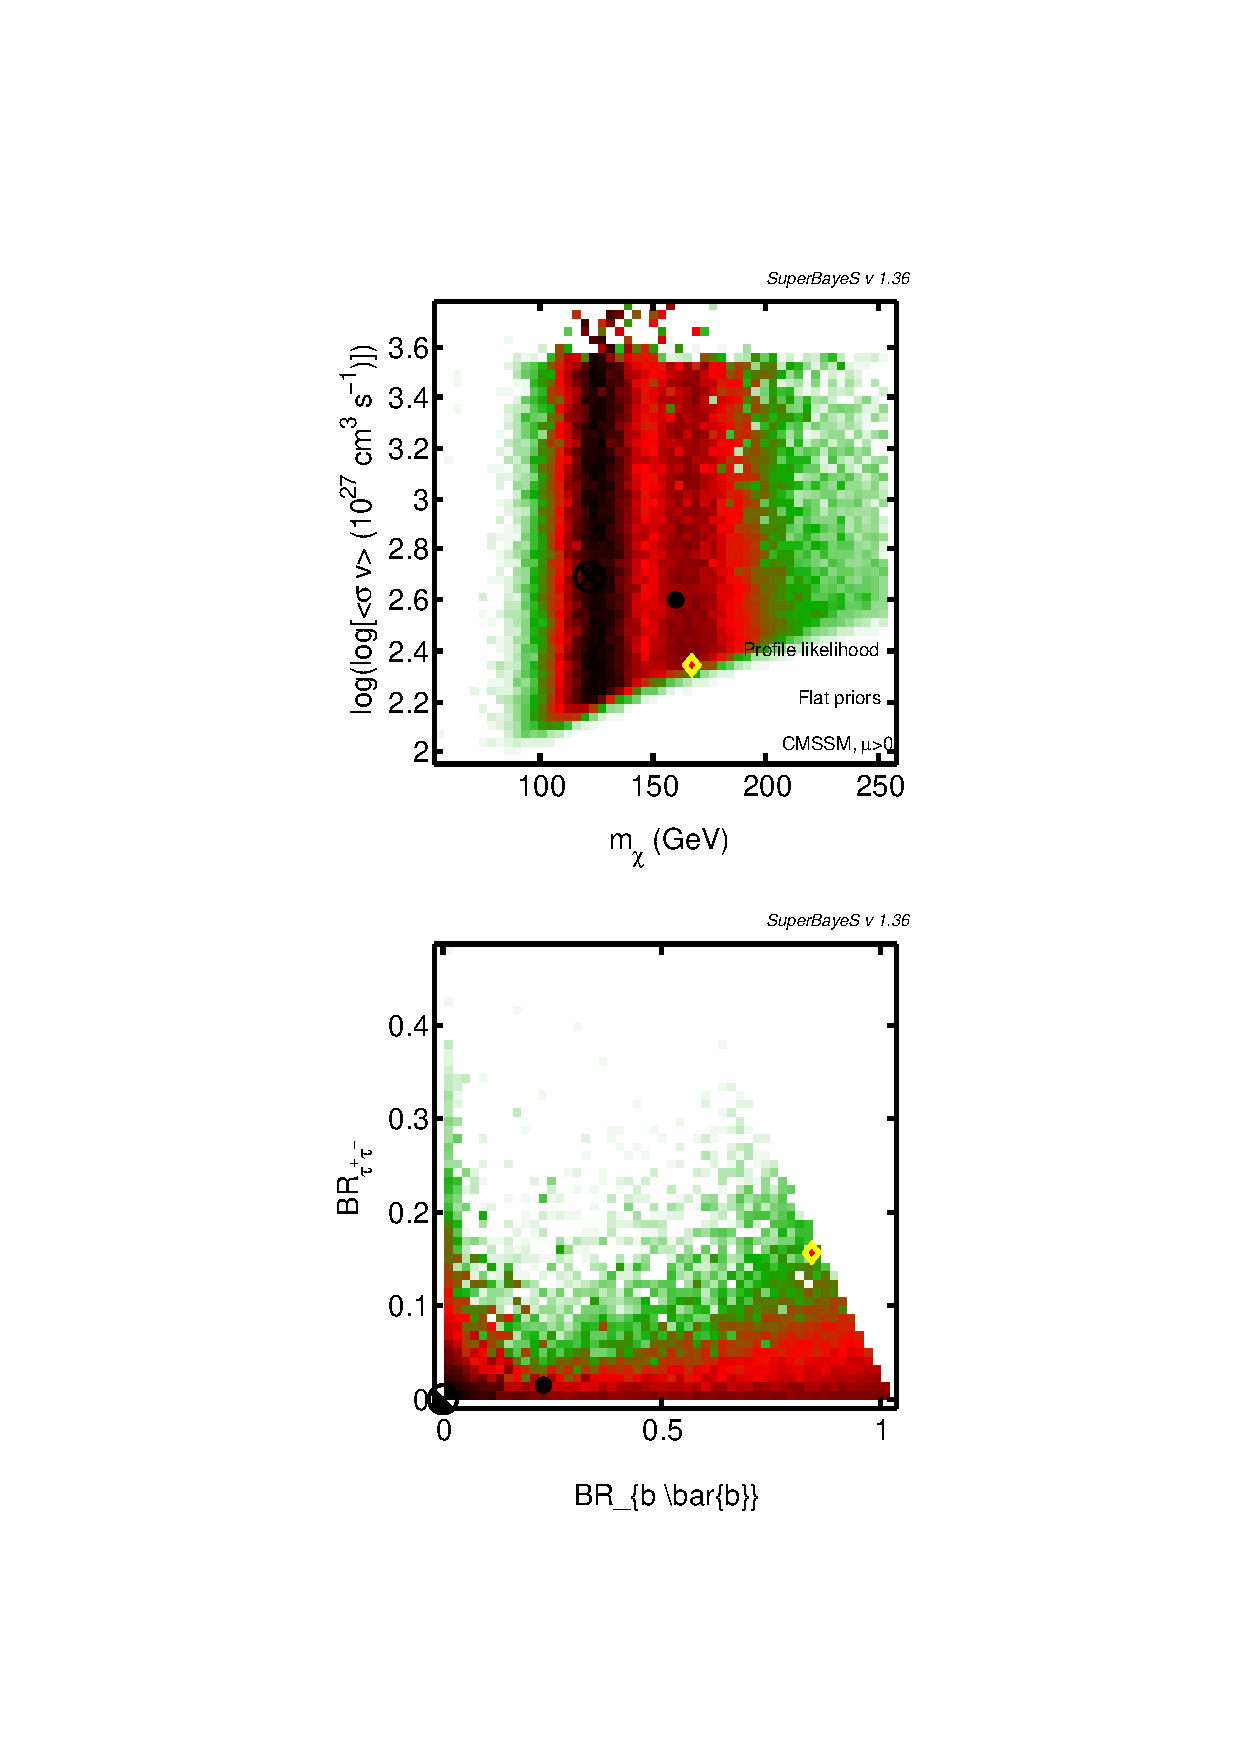
\includegraphics[trim = 140 120 140 120, clip = true, width=0.46\textwidth]{figs/2D_PL_PLscan}
\caption{Parameter inference results from a scan with PL set-up. The left (right) plots give marginalised posterior PDFs (profile likelihoods).  Crosses indicate the best fit, bullets the posterior mean, and red/yellow diamonds the true parameter values. (Ignore annotations referring to CMSSM and \textsc{SuperBayeS})}
\label{PLscan}
\end{figure} 

As can be seen, for a PL scan the parameter space around the true point is reasonably well sampled. The best fit point is still far away from the true point. This is most likely due to realisation noise in the simulated data. The posterior PDF is also still centred far away from the true point. To determine if the BRs are all reasonably well sampled within their allowed range [0,1] one can consider the 1D profile likelihood distributions, shown in Fig. \ref{1DPLBR}. \\
\begin{figure}
\centering
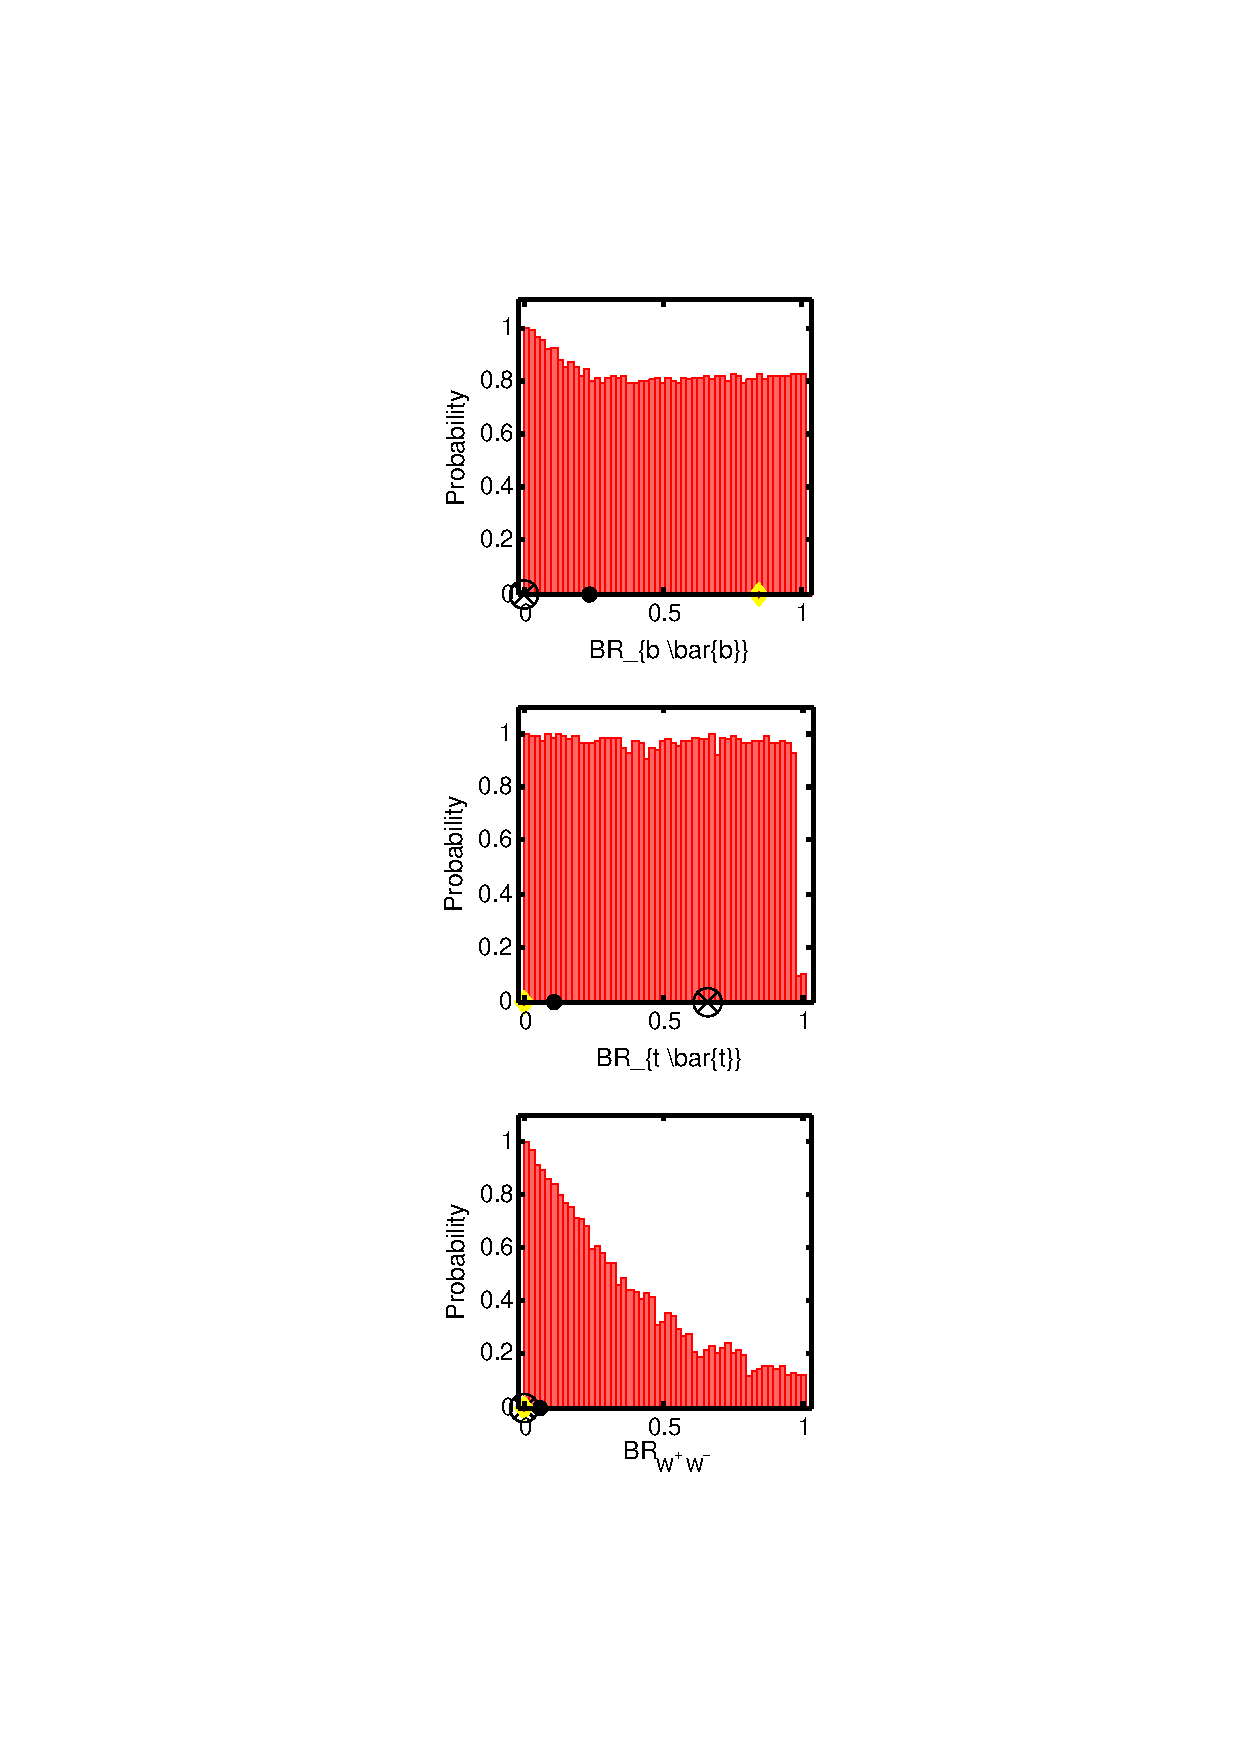
\includegraphics[trim = 205 100 202 100, clip = true, width=0.32\textwidth]{figs/1D_PL_BR_1_PLscan}
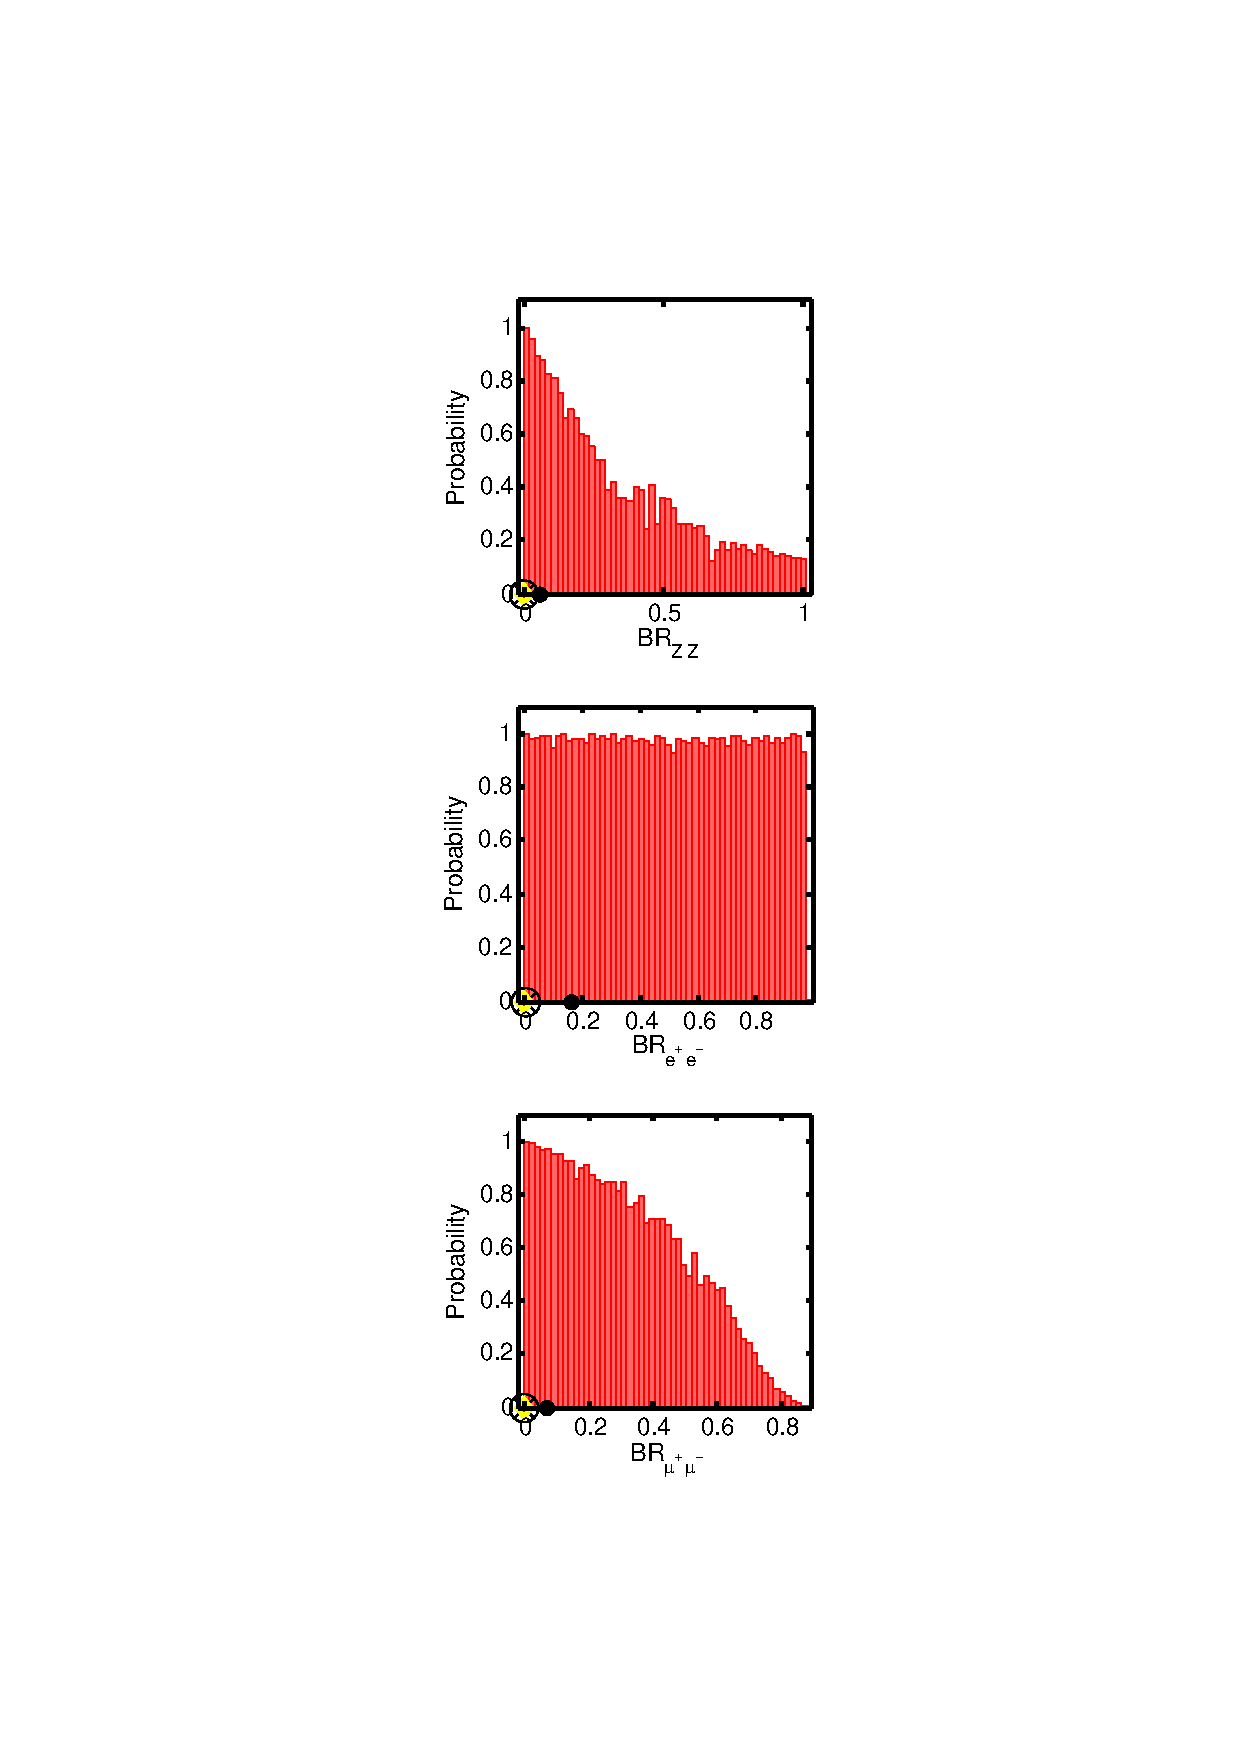
\includegraphics[trim = 205 100 202 100, clip = true, width=0.32\textwidth]{figs/1D_PL_BR_2_PLscan}
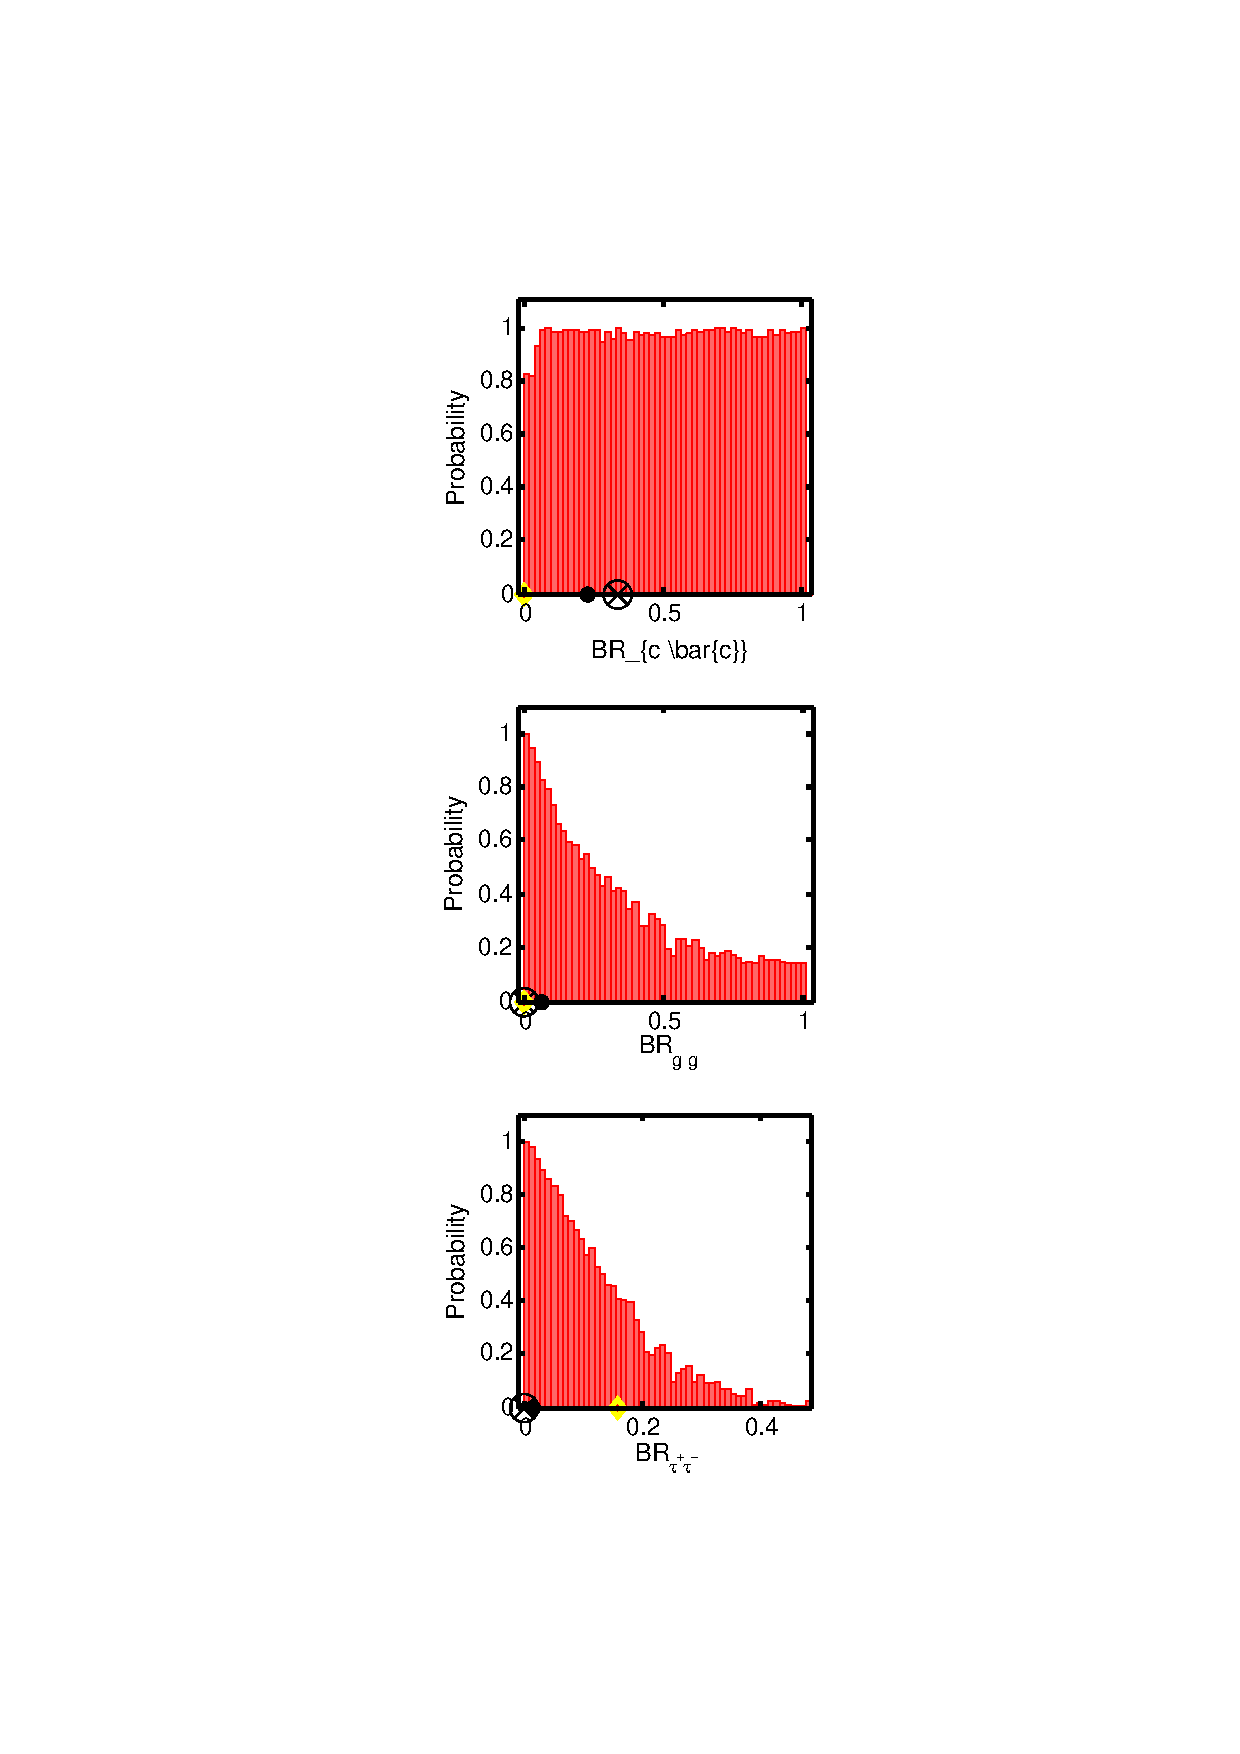
\includegraphics[trim = 205 100 202 100, clip = true, width=0.32\textwidth]{figs/1D_PL_BR_3_PLscan}
\caption{1D profile likelihood functions of the BRs resulting from a scan with PL set-up. Crosses indicate the best fit, bullets the posterior mean, and red/yellow diamonds the true parameter values. (Ignore annotations referring to CMSSM and \textsc{SuperBayeS})}
\label{1DPLBR}
\end{figure}

As can be seen, the profile likelihood distributions cover most of the parameter space. In order to fully cover the range [0,1] for each of the BRs, the scan will be repeated for three different effective priors and the resulting chains will be combined. The three priors will resemble the examples shown in Fig. \ref{BRPriorShape}. This will ensure that high, low and intermediate BR values are all well explored. The profile likelihood results from the combined chains can be used to infer the true values of the DM parameters.

The first effective prior on the BRs that will be used will have a similar shape as the distribution shown in the top plot in Fig. \ref{BRPriorShape}. This distribution corresponds to a small log(cross-section) range and will ensure that intermediate values of the BR are well-sampled. A useful quantity to investigate in order to determine which log(cross-section) range will lead to the best prior distribution to achieve this is the full width at half maximum (FWHM). The plot of the FWHM of the effective prior on the BRs as a function of the range of the log prior on the annihilation cross-sections is shown in in Fig. \ref{FWHM_plot} for six, seven, eight and nine open annihilation channels.
\begin{figure}
\centering
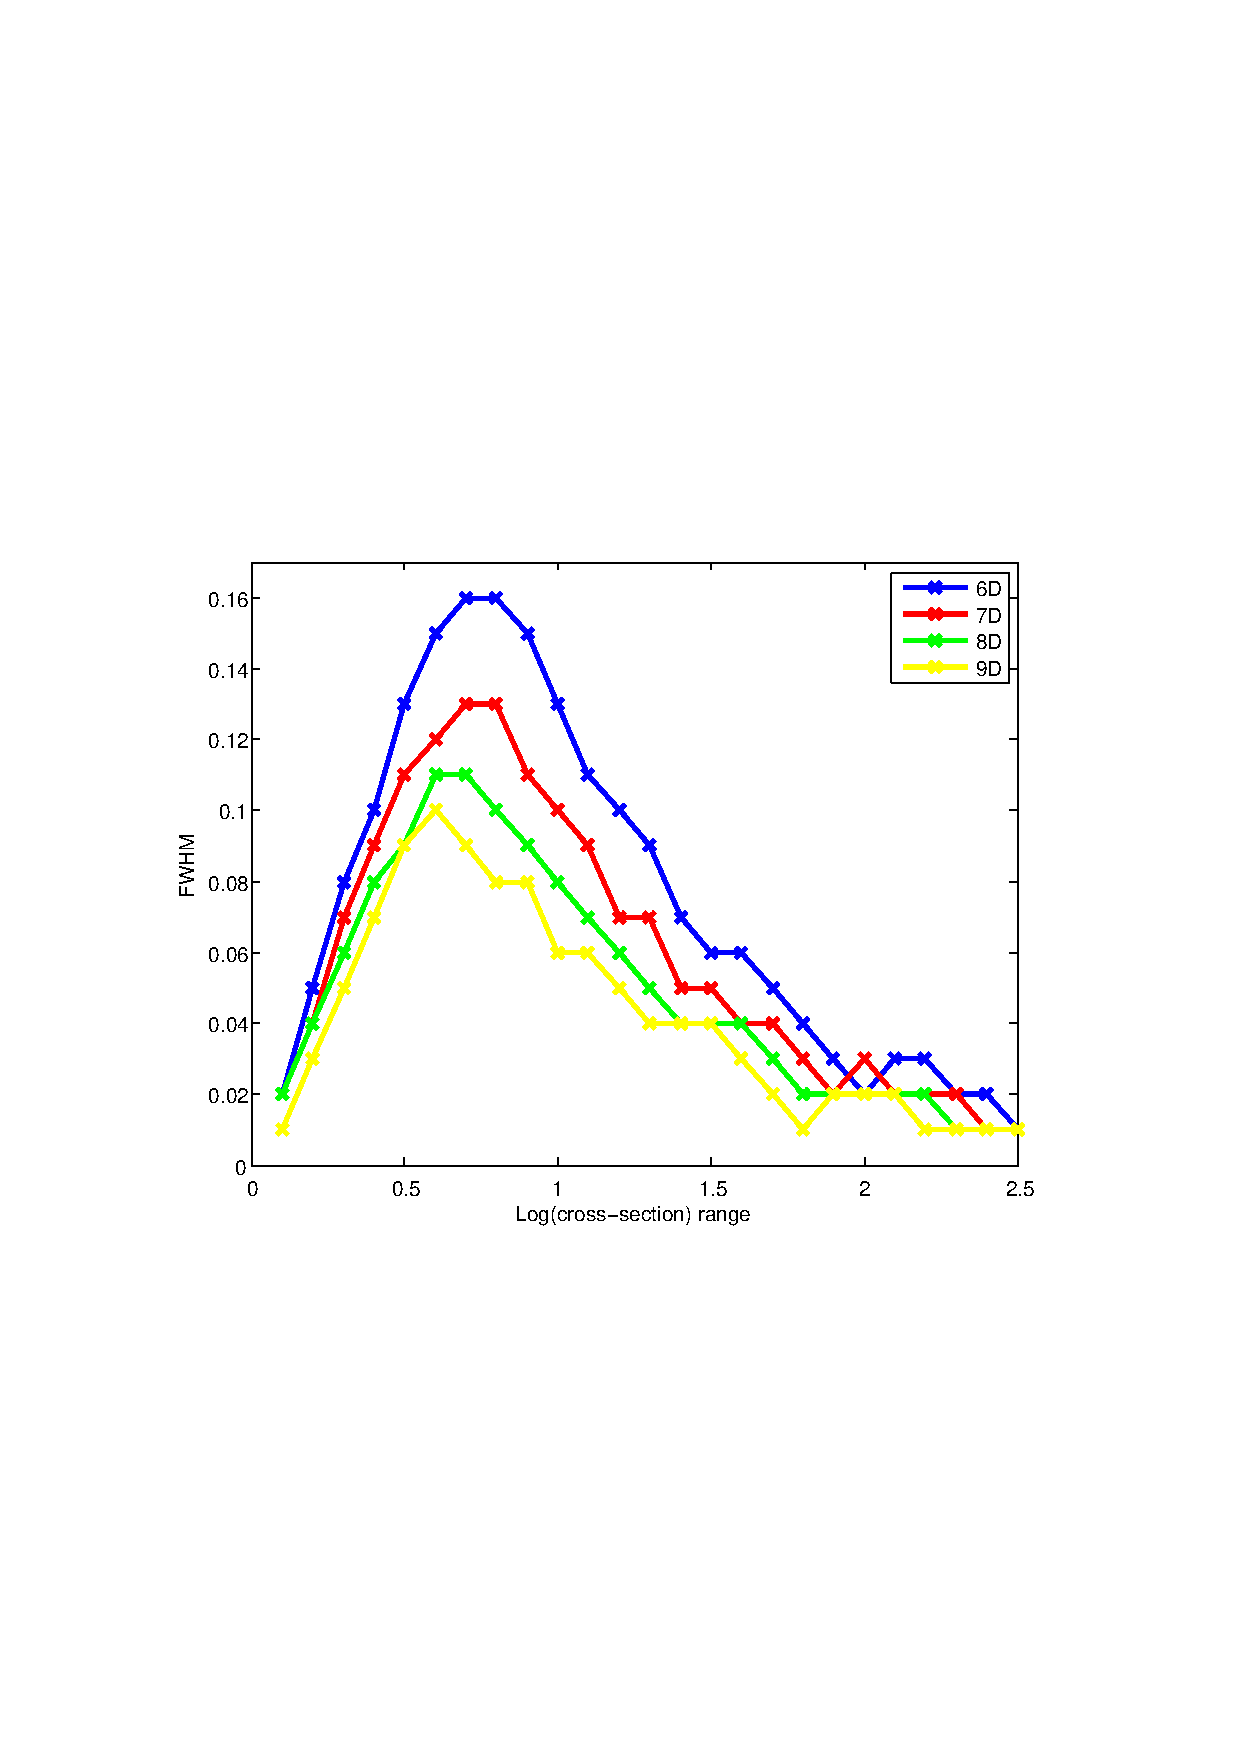
\includegraphics[trim = 70 240 90 240, clip = true, width=0.7\textwidth]{figs/FWHM_vs_Range}
\caption{FWHM as a function of range of the log prior on the cross-sections for the effective prior on the BRs. The distribution is given for six (blue), seven (red), eight (green) and nine (yellow) dimensions.}
\label{FWHM_plot}
\end{figure}
As a representative example, the data points in seven dimensions are given in table \ref{FWHM_7D}. The data in other dimensions show a similar behaviour.
\begin{table*}[htp]
\centering
\fontsize{9}{9}\selectfont
\begin{tabular}{c|c|c|c|}
\hline
\hline
 Log($\sigma_{\chi \chi \rightarrow r_i r_i}$) Range & Largest Bin Position & $\#$ Non-zero Bins & FWHM \\
\hline
0.1 & 15 & 5 & 0.02\\
0.2 & 14 & 11 & 0.04\\
0.3 & 13 & 16 & 0.07\\
0.4 & 12 & 22 & 0.09\\
0.5 & 11 & 27 & 0.11\\
0.6 & 10 & 33 & 0.12\\
0.7 & 9 & 39 & 0.13\\
0.8 & 8 & 44 & 0.13\\
0.9 & 7 & 50 & 0.11\\
1.0 & 6 & 55 & 0.10\\
1.1 & 5 & 61 & 0.09\\
1.2 & 5 & 65 & 0.07\\
1.3 & 4 & 70 & 0.07\\
1.4 & 4 & 75 & 0.05\\
1.5 & 3 & 78 & 0.05\\
1.6 & 3 & 82 & 0.04\\
1.7 & 2 & 85 & 0.04\\
1.8 & 2 & 87 & 0.03\\
1.9 & 2 & 89 & 0.02\\
2.0 & 2 & 91 & 0.03\\
2.1 & 2 & 93 & 0.02\\
2.2 & 2 & 94 & 0.02\\
2.3 & 1 & 95 & 0.02\\
2.4 & 1 & 96 & 0.01\\
2.5 & 1 & 97 & 0.01\\
\hline
\end{tabular}
\caption{\fontsize{9}{9}\selectfont FWHM of the effective prior on the BRs in 7D for different ranges of the log prior on the cross-section. Additionally, the position of the largest bin and the number of non-zero bins is given for each range.} 
\label{FWHM_7D}
\end{table*}

Each of the curves in Fig. \ref{FWHM_plot} have a similar shape, including a distinct peak. The higher the dimensionality of the parameter space, the the less pronounced is this peak. Additionally, the peak is shifted to slightly higher ranges as the dimensionality decreases. Given the shape of these distributions an obvious choice of effective prior for the BRs would be the distribution resulting from the log cross-section range at which the peak FWHM value is found. This is equivalent to maximising the number of bins containing a large number of points. However, it is important to keep in mind that both smaller and larger ranges for the log prior on the cross-sections have certain advantages. As can be seen in Table \ref{FWHM_7D}, the smaller the range, the more central is the position of the largest bin. Therefore, while the distribution does become narrower for smaller ranges, more central values of the BRs may be better sampled. On the other hand, the larger the range, the larger the number of bins that contain a non-zero number of points. Therefore, the overall number of BR values sampled increases, even though they might not be sampled as well as for smaller cross-section ranges.

The second effective prior on the BRs that is of interest resembles the shape of the distribution shown in the central plot of Fig. \ref{BRPriorShape}. This prior distribution would lead to intermediate and large BR values being equally well sampled. To investigate which range for the log prior on the cross-section to choose to obtain this effective prior one can consider the ratio of the size of the last bin (BR = [0.99,1.0]) to the size of the smallest bin. This ratio is shown in Fig. \ref{Bin100_Binsmallest} as a function of the range of the log prior on the cross-sections for different dimensionalities of the parameter space.  
\begin{figure}
\centering
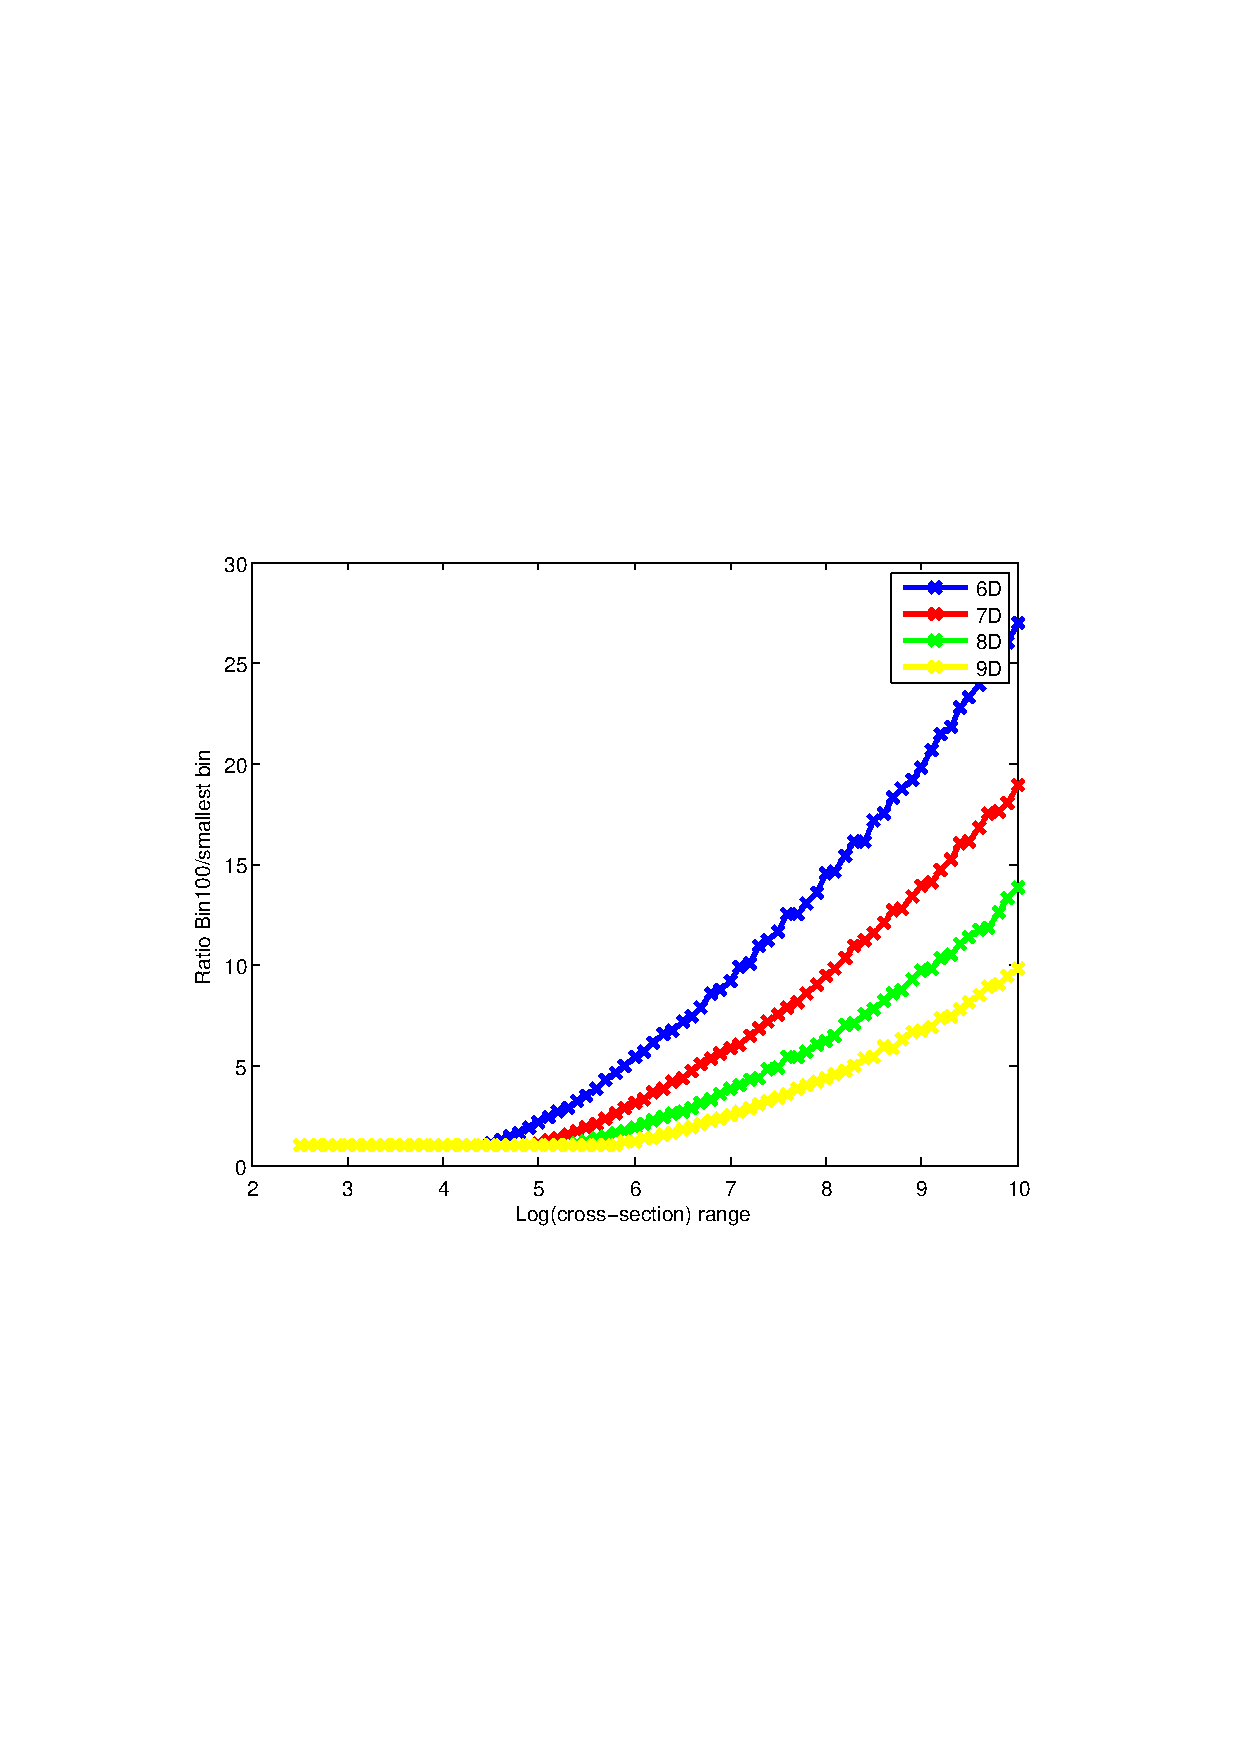
\includegraphics[trim = 70 240 90 240, clip = true, width=0.9\textwidth]{figs/Ratio_Bin100_Binsmallest}
\caption{Ratio of the size of the last bin (BR = [0.99,1.0]) to the size of the smallest bin as a function of range of the log prior on the cross-sections for the effective prior on the BRs. The distribution is given for six (blue), seven (red), eight (green) and nine (yellow) dimensions.}
\label{Bin100_Binsmallest}
\end{figure}
As can be seen, this ratio is equal to unity for small ranges, since for these ranges the last bin and the the smallest bin are identical. At some range the ratio becomes larger than unity, because the size of the last bin is now larger than the size of the smallest bin. As can be seen, the larger the number of free BRs, the larger the range of the log prior on the annihilation cross-sections at which this ratio becomes greater than unity.

Another interesting quantity to consider in order determine which range leads to the best sampling of the parameter space is the ratio of the size of the smallest bin to the size of the first bin (BR = [0.0,0.01]). In Fig. \ref{Binsmallest_Bin1} this ratio is shown as a function of the range of the log prior on the annihilation cross-sections for different numbers of free BRs.
\begin{figure}
\centering
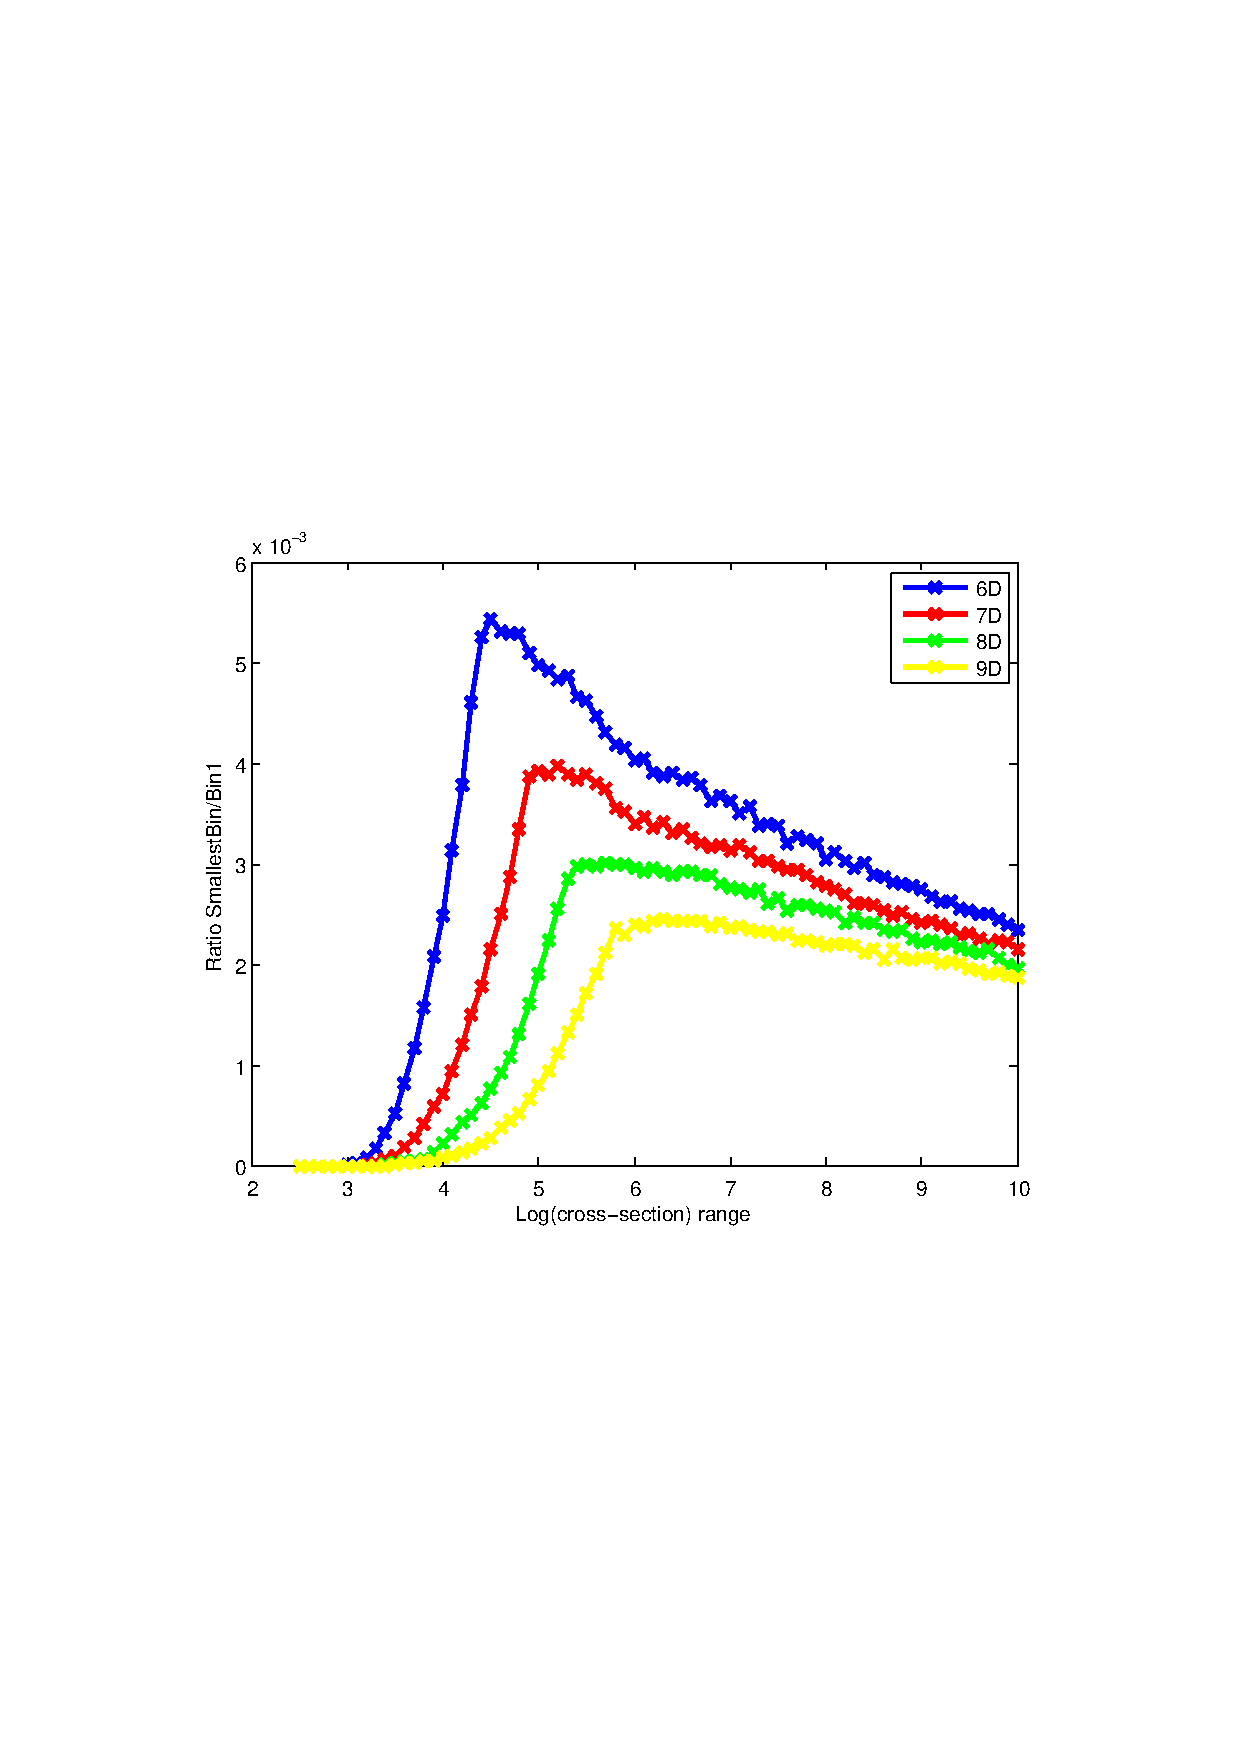
\includegraphics[trim = 70 240 90 240, clip = true, width=0.9\textwidth]{figs/Ratio_Binsmallest_Bin1}
\caption{Ratio of the size of the smallest bin to the size of the first bin (BR = [0.0,0.01]) as a function of range of the log prior on the cross-sections for the effective prior on the BRs. The distribution is given for six (blue), seven (red), eight (green) and nine (yellow) dimensions.}
\label{Binsmallest_Bin1}
\end{figure}
The distribution is peaked around a certain range value, which shifts towards higher ranges as the dimensionality of the parameter space increases. By comparing Fig. \ref{Binsmallest_Bin1} and Fig. \ref{Bin100_Binsmallest} one can see that the peak occurs at similar (slightly higher) ranges as the range at which the smallest bin position starts to move towards more central values of the BRs. Therefore, a good choice of effective prior for the BRs in each dimension would be the distribution resulting from the range of the log prior on the cross-sections at which the peak of the ratio of size of the smallest bin to the size of the first bin is found.

When trying to choose the most convenient such prior by using ratios involving the size of the smallest bin, it is useful to keep track of the position of this bin. This position as a function of range of the log prior on the cross-sections can be seen in Fig. \ref{Minbin Position}.
\begin{figure}
\centering
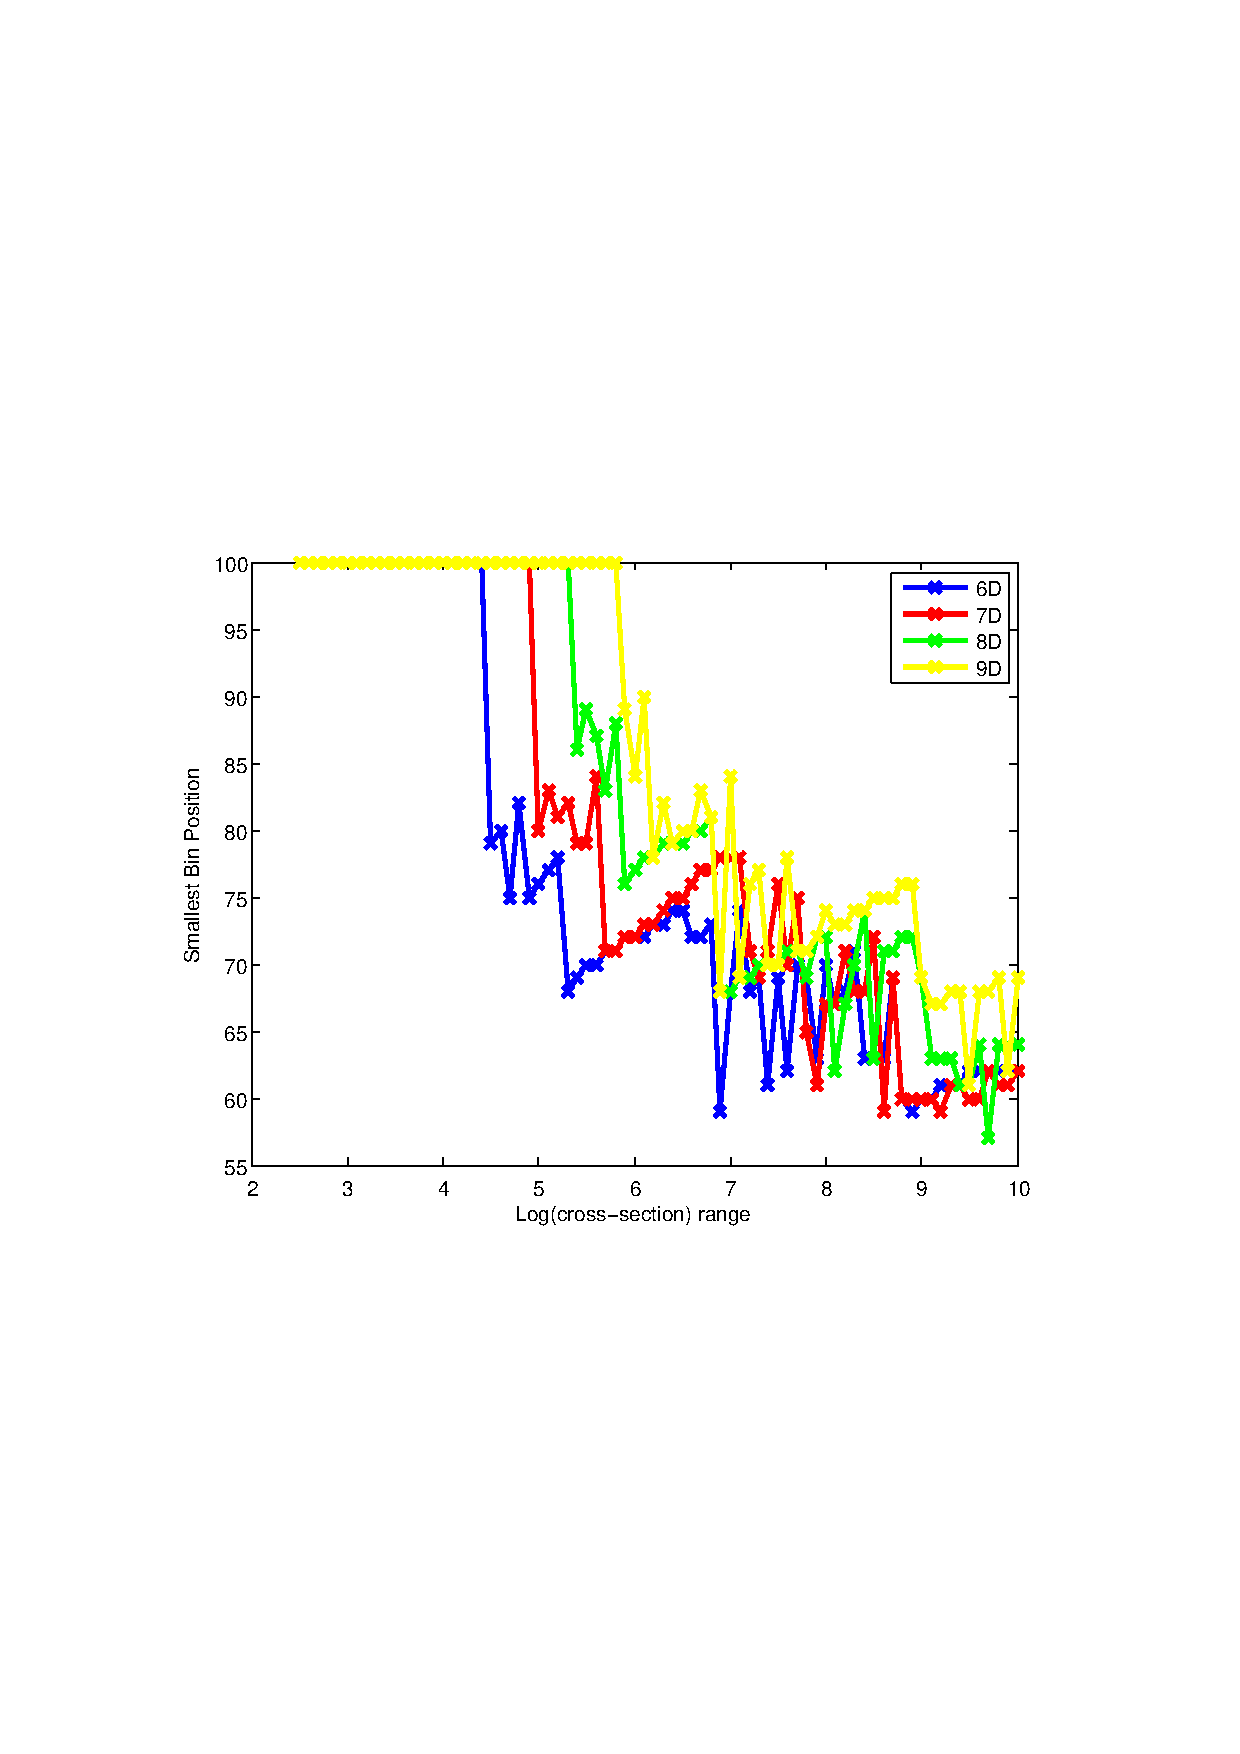
\includegraphics[trim = 70 240 90 240, clip = true, width=0.9\textwidth]{figs/Min_bin_vs_Range}
\caption{Position of the smallest bin as a function of range of the log prior on the cross-sections for the effective prior on the BRs. The distribution is given for six (blue), seven (red), eight (green) and nine (yellow) dimensions.}
\label{Minbin Position}
\end{figure}
Even though there is a relatively large scatter in the position of the smallest bin as a function of range, one can clearly see that the position of the smallest bin shifts towards more central values of the BRs as the range of the log prior on the annihilation cross-sections increases.

The third type of prior that we want to use will resemble the shape of the distribution shown in the bottom plot in Fig. \ref{BRPriorShape}. Such a distribution corresponds to an effective prior on the BRs that will mostly sample extreme values of the BRs, i.e.\ both very high or very low values. In order to choose a range of the log prior on the cross-sections leading to such a distribution one can consider the ratio of the size of the last bin (BR = [0.99,1.0]) to the size of the first bin (BR = [0.0,0.01]). The plot of this ratio as a function of the range of the log prior on the annihilation cross-sections is given in Fig. \ref{Bin100Bin1} for different dimensionalities of the parameter space.
\begin{figure}
\centering
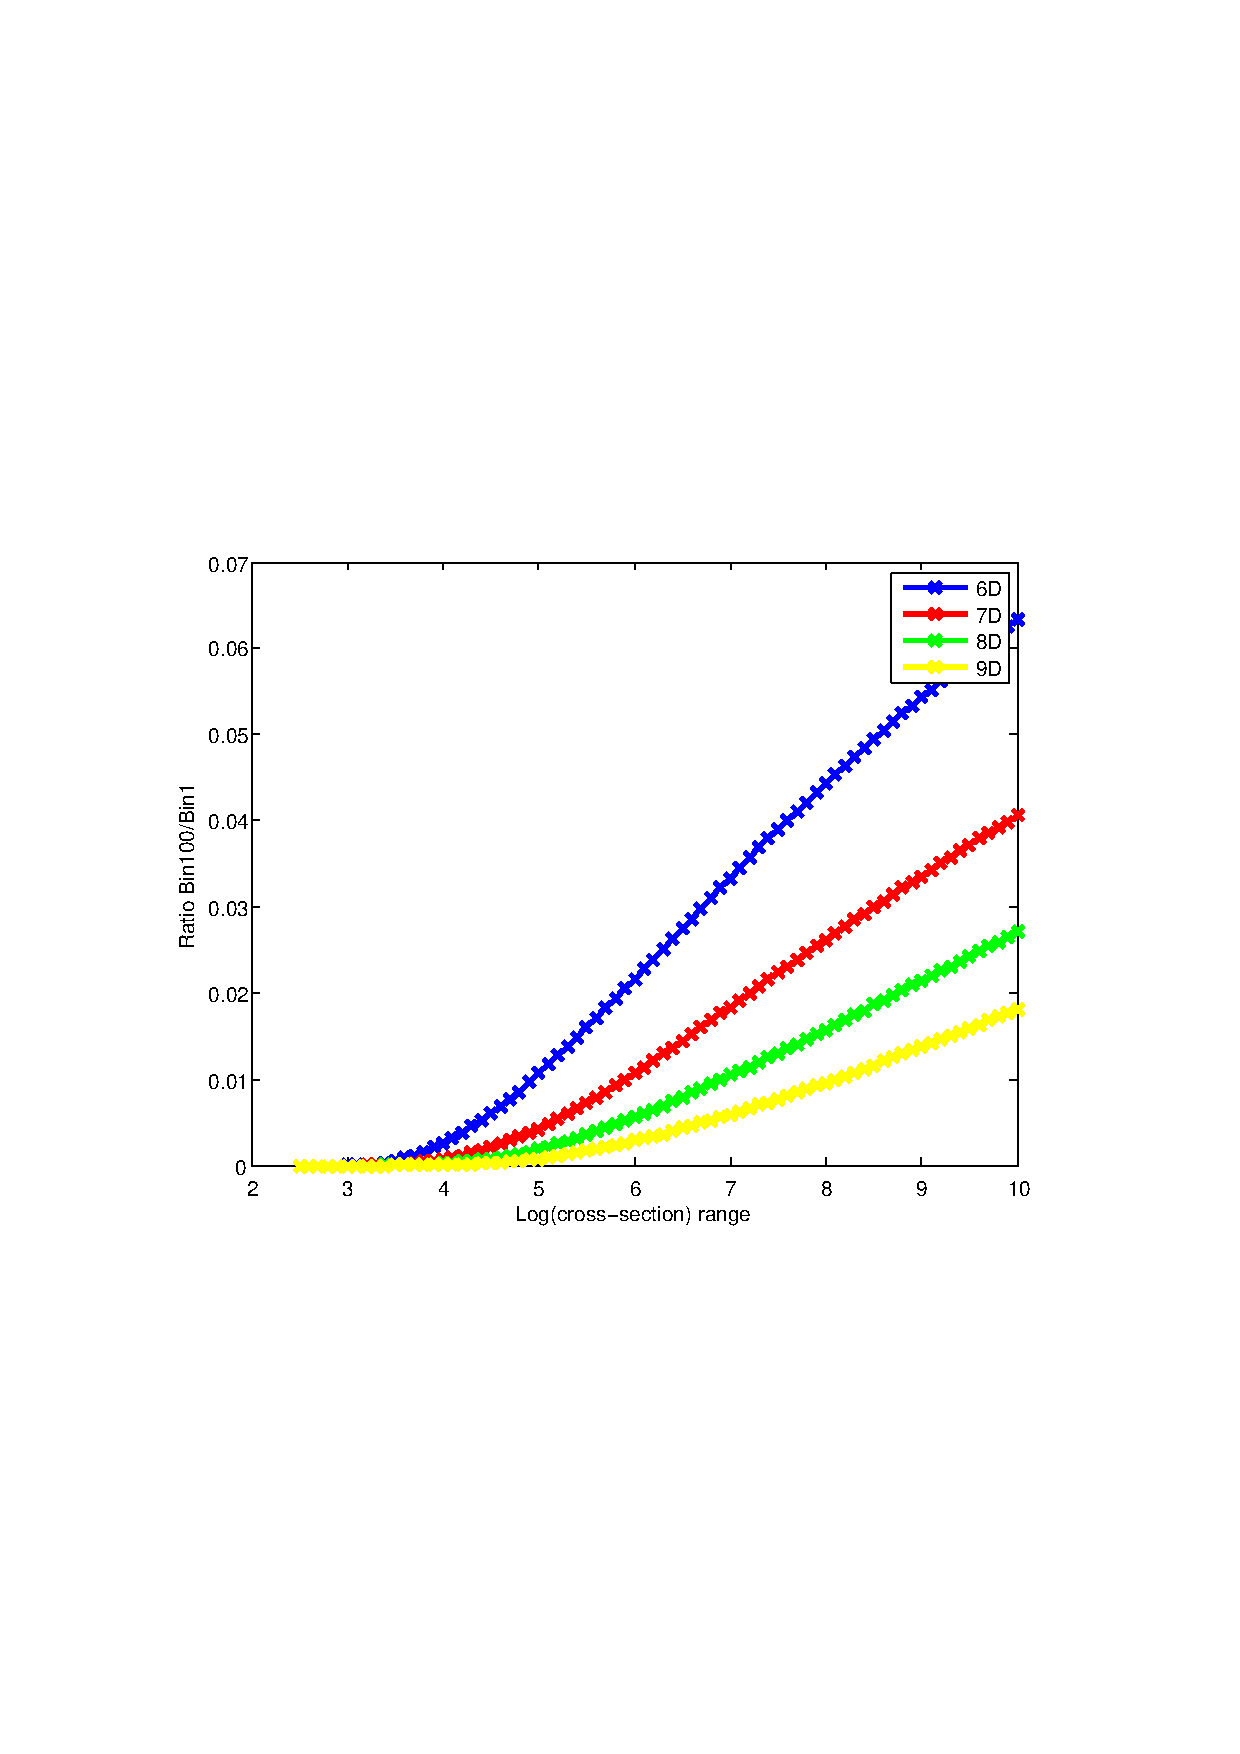
\includegraphics[trim = 70 240 90 240, clip = true, width=0.9\textwidth]{figs/Ratio_Bin100_Bin1}
\caption{Ratio of the size of the last bin (BR = [0.99,1.0]) to the size of the first bin (BR = [0.0,0.01]) for the effective prior distribution on the BRs as a function of range of the log prior on the cross-sections. The distribution is given for six (blue), seven (red), eight (green) and nine (yellow) dimensions.}
\label{Bin100Bin1}
\end{figure}
As can be seen, this ratio is zero for small ranges, since the last bin does not contain any points. The range at which this ratio becomes non-zero increases as the number of free BRs increases. Once the ratio is non-zero it steadily grows with the range of the log prior on the cross-sections. Therefore, the higher the range, the better sampled are high values of the BRs. However, one should keep in mind that the larger the range, the more the distribution is concentrated at very low and very high values of the BRs, and thus the smaller the number of bins that are well-sampled.

\cs{The most important questions are:
\begin{itemize}
	\item Small range prior: Should we use the distribution resulting from the log cross-section range at which the peak FWHM value is found? Smaller ranges would lead to a more central position of the largest bin, but would also lead to a smaller BR range being sampled. Larger ranges would lead to a larger sampled BR range, but the number of bins with a high number of points decreases and the maximum of the distribution is shifted to lower values of the BRs.
	\item Medium range prior: I recommend using the distribution resulting from the range of the log prior on the cross-sections at which the peak of the ratio of size of the smallest bin to the size of the first bin is found as the second effective prior for the BRs. What do other people think?
	\item Large range prior: Which range of the log prior on the cross-sections should we choose for the third type of prior? The higher the range, the better very high values of the BRs are sampled (the larger the ratio of the size of the last bin to the size of the first bin). However, the larger the range, the smaller the number of bins that is well-sampled. What is a good criterion to choose the range for this prior?
\end{itemize}
}

\subsection{Background modelling}

\subsubsection{Set-up}
The background models depend non-linearly on some parameters, whereas the dependence on others can be approximated by a linear or power-law scaling. For the non-linear parameters ({\bf grid parameters}), we generated a grid of mapcubes that covers reasonable variations of the background model with these parameters. Each grid point has a set of template maps associated with it, each representing a contribution to the total flux. Each template map is rescaled by the appropriate linear/power-law parameters ({\bf template parameters}), then the 14 rescaled template maps are added together to give the total flux for the considered grid point. The correct flux map for every point in parameter space can the be found by {\bf linear interpolation} between the grid points. A typical interpolation within this two-step model happens as follows:
\begin{enumerate}
\item Choose a specific combination of grid parameters $\theta_g$, and a specific combination of template parameters $\theta_t$ (i.e.\ a single point in the full (1 + 10)D background parameter space).
\item Identify the points in the grid defining the hypercube surrounding $\theta_g$.
\item For all vertices of that hypercube, use $\theta_t$ to compute the scaled template contributions to the total background model at each vertex.
\item At each vertex, add the fluxes of the respective template contributions to obtain the total background model at that vertex.
\item Linearly interpolate the resulting total background maps from these vertices to the chosen point in the grid $\theta_g$.
\end{enumerate}

We have decided on a spatial pixel size of 0.25 $\times$ 0.25 degrees, 15 log-spaced energy bins from 300\ MeV to 100\ GeV, and a 15 $\times$ 15 degrees ROI for PSF convolution -- of which a 10 $\times$ 10 degree region will be used for the likelihood calculation.

\subsubsection{Detailed description of the background model parameters}

   In its simplest form, the ISM background model is a line of sight integral
   of the product of target density and CR density.  Unfortunately, neither is
   known with great accuracy.

\subsubsection*{Target distributions} 
   
   The two big contributors in the ISM are hydrogen and helium gas.  Cold helium
   cannot be observed so it is usually assumed to have the same distribution
   as hydrogen.  Hydrogen in the ISM has three forms: atomic, molecular, and
   ionised.  Atomic hydrogen is observed with the 21-cm hyperfine line that has to
   be corrected for optical depth.  That is done using the spin temperature
   $T_S$ under the assumption of uniform $T_S$ along the line of sight (for
   that particular Doppler shift of the 21-cm line).  The H\,\textsc{i} column density is
   given with
   \begin{equation}
      N(HI) = -\log\left(1-\frac{T}{T_S - T_{bg}}\right) T_S C
      \label{eq:spinTemperature}
   \end{equation}
   where $T$ is the line temperature, $C = 1.83\times10^{18}$~cm$^{-2}$ K
   (km/s)$^{-1}$, and $T_{bg}$ is the
   background temperature, usually assumed to be the CMB background.  For $T_S
   \rightarrow \infty$ we have $N(HI) \propto T$ while when $T_S \rightarrow
   T+T_{bg}$ we have $N(HI) \rightarrow \infty$.  To have a more linear
   parameter in the grid, we actually scan over 
   \begin{equation}
    x_S \equiv \left(\frac{T_S}{K}\right)\log_{10}\left[1-\left(\frac{80K}{T_S}\right)\right],
   \end{equation}
   instead of $T_S$ itself.

   The molecular hydrogen is not directly observed so we use CO maps as a proxy for the H$_2$ distribution.
   We use a linear approximation to turn integrated CO line intensity, $W(CO)$,
   into column density $N(H_2) = X_{CO} W(CO)$.  There is some evidence that
   $X_{CO}$ is variable over the Galaxy and this is especially true close to
   the GC.

   We use the Doppler shift of the lines to place the gas along the line of
   sight assuming the gas is rotating around the GC.  This method breaks down
   close to the GC (within $\sim 10^\circ$) and we use linear interpolation
   from surrounding areas.  The distribution of gas is therefore highly
   uncertain in the ROI.

\subsubsection*{CR distribution}
   
   The distribution of CRs depends on the distribution of sources and their
   propagation throughout the Galaxy.  To simplify things, we assume we know
   the propagation and only adjust the source distribution.  This is of course a
   simplification, but should suffice to parameterise the uncertainty of the
   background model.  We go a step further and adjust the propagated CR flux
   with a functional form
   \begin{equation}
      CR(R) \propto \left(\frac{R}{R_\odot}\right)^\alpha
      e^{-\beta\frac{R-R_\odot}{R_\odot}}
      \label{eq:CRsourceDistribution}
   \end{equation}
   We'll start by changing only $\alpha$ with a fixed $\beta$, basically controlling
   the peakiness of the CR source distribution.  The lower the value of
   $\alpha$, the peakier the distribution gets.  We use the same distribution
   for the CR sources as in GALPROP.  The distribution of CRs is
   supposed to include uncertainty in the distribution of targets as well.
   Due to our limited source distribution function, this might not be
   accurate.

\subsubsection*{Some approximations we apply}

   To make the runs simpler, we do not include secondary electrons and
   positrons.  They mostly affect the ISM model at low energies and we are
   anyway focused on the DM limits, not the background model.  Since they are
   generated from CR protons, we would have to split the electron components
   into secondary and primary components and add them to the proton component.
   This can be done but introduces more parameters (and work).

   To simplify things we change the spectral index of the final products
   rather than the injected CRs.  This is accurate when the propagation only
   changes the power law index of the injected spectrum, which holds pretty
   well in the energy range from a few\ GeV to few hundred\ GeV for electrons
   and few TeV for protons.  This is in fact the energy range we are
   considering for this analysis so it should be safe.  Note that when we
   change the spectrum we have to allow for freedom in the normalisation as
   well, that is we multiply the templates with $f(E) = f_0 * E^i$ where $f_0$
   and $i$ are free parameters.

\subsubsection{Specifics of particular grid setups}

   {\bf Test Grid I }
   
   The directory bg$\_$data contains a subfolder TestGridI. This folder contains the test grid. This folder contains one subfolder for each grid point corresponding to different values of the grid parameter(s), which contains the template .fits files for the grid point. TestGridI also contains an index file; the location of the index file for a scan will be given in the .ini file. The index file contains information about the number of grid and template parameters, the number of templates and the parameter names. It also contains the values of the grid parameters associated with each grid point, the type of template parameter (linear or special), and the templates rescaled by each template parameter. In order to implement the BG parameters in the code two new parameter types (Grid$\_$params, Template$\_$params) were defined. \\

The following model currently stored in TestGridI:

   {\em Grid parameters:}
   \begin{itemize}
      \item Spin temperature, $T_S$
   \end{itemize}
   
   {\em Template parameters:}
   \begin{itemize}
      \item CR proton source distribution ($\alpha$, and/or $\beta$)
      \item CR proton spectra index and normalisation
      \item CR electron spectral index and normalisation
      \item $X_{CO}$ parameters, one for each of 0--1.5\,kpc, 1.5--3\,kpc, 3--50\,kpc
   \end{itemize}

   There are 6 values of $T_S$ for this model so only 6 grid points.  The
   templates for each grid point is stored in a separate directory, called
   TestGridI\_<i>, where i is a grid index going from 1 to 6. Each of the template map cubes has 0.25 degree pixel resolution and spans [-15,15] degrees. The mapping to  $T_S$ (and $x_{S}$) values is as follows: \\
  
   \begin{tabular}[h]{c|c|c}
      Grid index & $T_S$ [K] & $x_{S}$\\
      \hline
      1 & 100 & -69.9 \\
      2 & 125 & -55.5 \\
      3 & 150 & -49.6 \\
      4 & 200 & -44.4 \\
      5 & 400 & -38.8 \\
      6 & 100000 & -34.8 \\
   \end{tabular}\\
   
  Each grid point has 13 template maps associated with it, created by summing up various GALPROP
   output components.  There is also one additional template map, identical at each grid point, associated with the Fermi bubbles. \ps{This 14th template still needs to be added.}  
   The template filenames are TestGridI\_<i>\_<j>, where j
   is a template index going from 1 to 13.  The mapping between templates and
   the index is:\\
   
   \begin{tabular}[h]{c|c}
      Template index & Description \\
      \hline
      1 & Bremss for HI and HII and ics \\
      2 & Bremss for H$_2$ from 0--1.5\,kpc \\
      3 & Bremss for H$_2$ from 1.5--3\,kpc \\
      4 & Bremss for H$_2$ from 3--30 \,kpc \\
      5 & $\pi^0$-decay for HI an HII from 0--3\,kpc \\
      6 & $\pi^0$-decay for HI an HII from 3--5\,kpc \\
      7 & $\pi^0$-decay for HI an HII from 5--10\,kpc \\
      8 & $\pi^0$-decay for HI an HII from 10--30\,kpc \\
      9 & $\pi^0$-decay for H$_2$ from 0--1.5\,kpc \\
     10 & $\pi^0$-decay for H$_2$ from 1.5--3\,kpc \\
     11 & $\pi^0$-decay for H$_2$ from 3--5\,kpc \\
     12 & $\pi^0$-decay for H$_2$ from 5--10\,kpc \\
     13 & $\pi^0$-decay for H$_2$ from 10--30\,kpc \\
     14 & Fermi bubbles \\
   \end{tabular}\\
   
   Templates 1--4 should be multiplied with the CR electron spectral index
   (correction) and normalization.  Templates 2--4 should be multiplied with
   $X_{CO}$ factors, one factor for each template.  The same $X_{CO}$ factors
   should be applied to templates 9--13, where the same $X_{CO}$ factor is
   used for templates 11--13.  Templates 5--13 should be multiplied with the CR proton spectra index and
   normalization.  These templates should also be corrected for the proton CR
   source distribution.  We pick a reference $R$ value for each template to calculate the normalization (\ar{$E_{0} = 3.405$\ GeV, $R_{0} = 8.5$\,kpc in fermi$\_$ini.f90::GC$\_$BG$\_$rescaled}).

\begin{tabular}[h]{c|c}
\hline
Template multiplied by rescaling factor & rescaling factor \\
\hline
1-4 & $\left(\frac{E_{center}}{E_{0}}\right)^{index_e}$ \\
1-4 & $norm_e$ \\
2,9 & $X_{CO,1}$ \\
3,10 & $X_{CO,2}$ \\
4,11,12,13 & $X_{CO,3}$ \\
5-13 & $norm_p$ \\
5-13 & $\left(\frac{E_{center}}{E_{0}}\right)^{index_p}$ \\
5-13 & $\frac{(R/R_{0})^{\alpha} \cdot exp(- \beta (R-R_{0})/R_{0}) }{(R/R_{0})^{2} \cdot exp(- 5 (R-R_{0})/R_{0}) }$ \\
\end{tabular} \\
\\
As an example, the 13 template maps associated with grid point 3 are given in Fig. \ref{TM1} - \ref{TM13}. For each template map two plots are shown. The left-hand plot corresponds to the first (lowest) energy bin, the right-hand plot corresponds to the last (highest) energy bin.
\begin{figure}
\centering
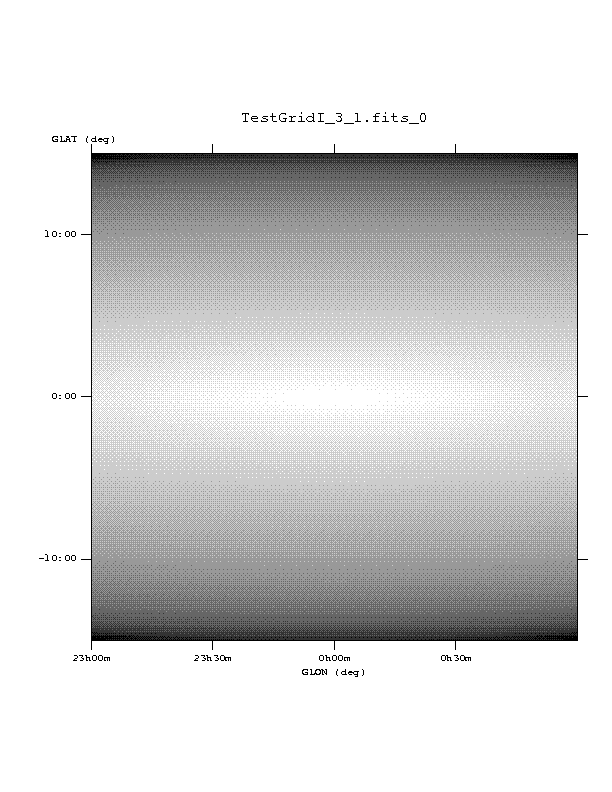
\includegraphics[trim = 50 100 70 100, clip = true, width=0.45\textwidth]{figs/Template_maps/Template1_Ebin01}
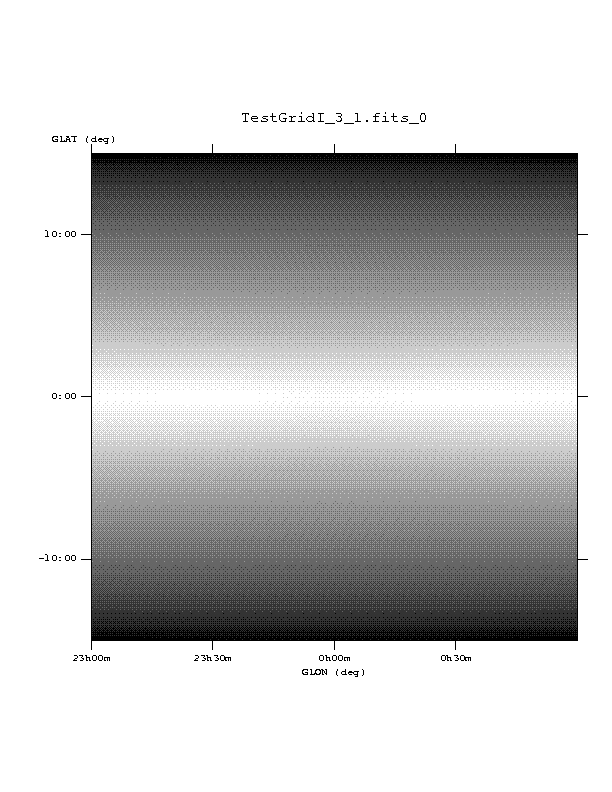
\includegraphics[trim = 50 100 70 100, clip = true, width=0.45\textwidth]{figs/Template_maps/Template1_Ebin71}
\caption{Template 1 flux maps for the first (left) and last (right) energy bin. The flux range is flux = $[6.75 \cdot 10^{-7}, 4.41 \cdot 10^{-6}]$ (flux = $[5.13 \cdot 10^{-18}, 1.21 \cdot 10^{-16}]$) in the first (last) energy bin.}
\label{TM1}
\end{figure}
\begin{figure}
\centering
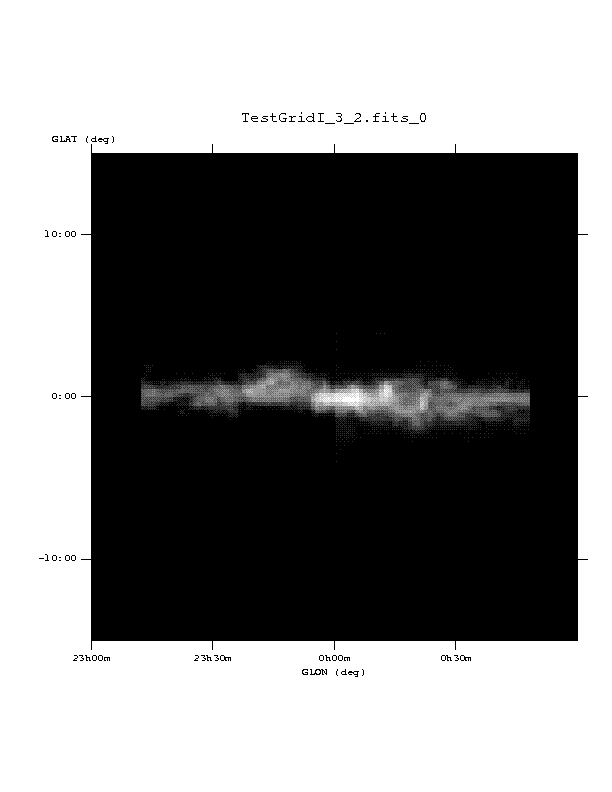
\includegraphics[trim = 50 100 70 100, clip = true, width=0.45\textwidth]{figs/Template_maps/Template2_Ebin01}
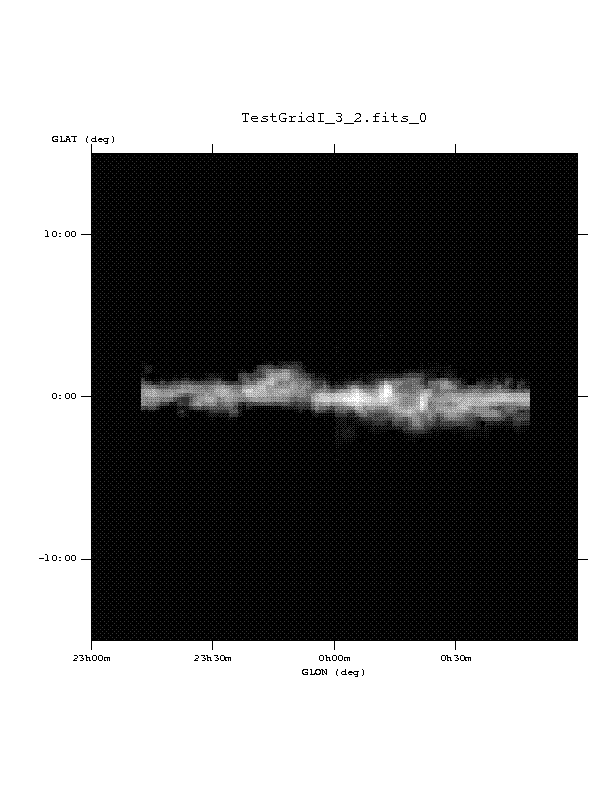
\includegraphics[trim = 50 100 70 100, clip = true, width=0.45\textwidth]{figs/Template_maps/Template2_Ebin71}
\caption{Template 2 flux maps for the first (left) and last (right) energy bin. The flux range is flux = $[-9.47 \cdot 10^{-9}, 5.58 \cdot 10^{-5}]$ (flux = $[-7.30 \cdot 10^{-21}, 1.35 \cdot 10^{-17}]$) in the first (last) energy bin.}
\end{figure}
\begin{figure}
\centering
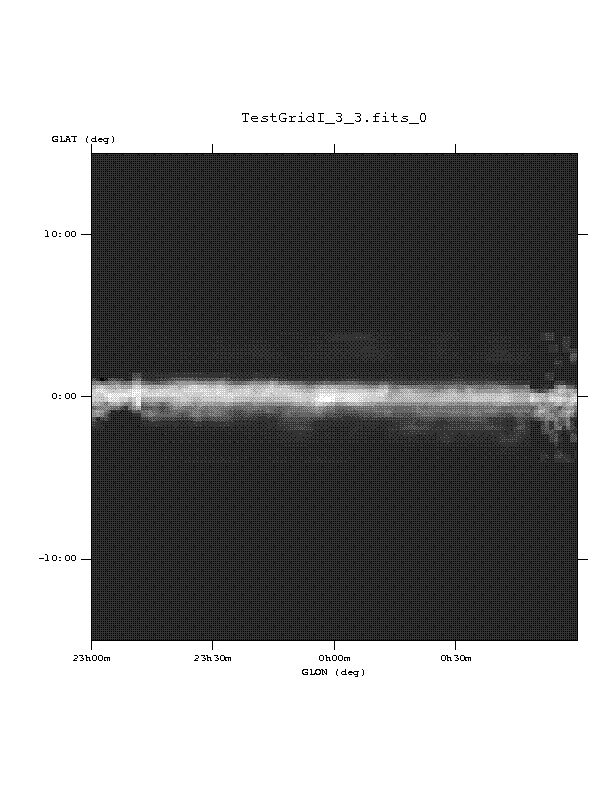
\includegraphics[trim = 50 100 70 100, clip = true, width=0.45\textwidth]{figs/Template_maps/Template3_Ebin01}
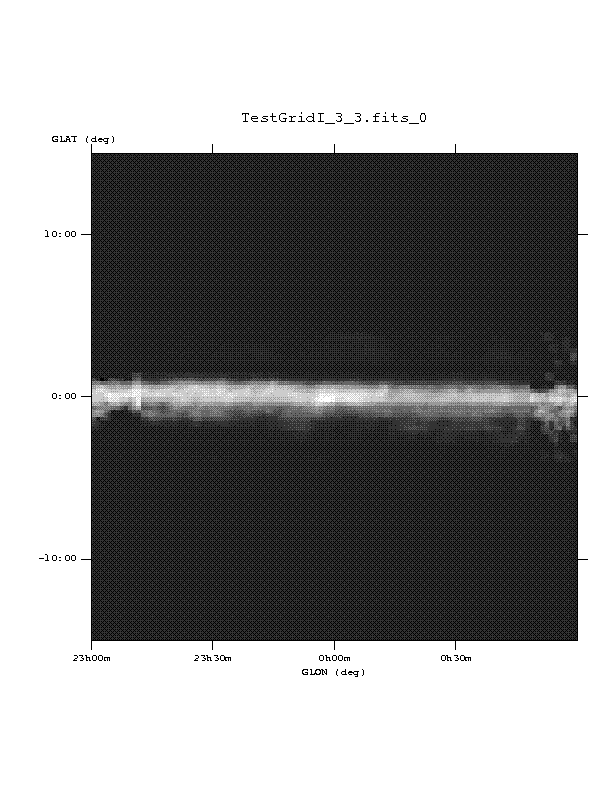
\includegraphics[trim = 50 100 70 100, clip = true, width=0.45\textwidth]{figs/Template_maps/Template3_Ebin71}
\caption{Template 3 flux maps for the first (left) and last (right) energy bin. The flux range is flux = $[-2.06 \cdot 10^{-8}, 3.83 \cdot 10^{-6}]$ (flux = $[-2.38 \cdot 10^{-20}, 5.45 \cdot 10^{-18}]$) in the first (last) energy bin.}
\end{figure}
\begin{figure}
\centering
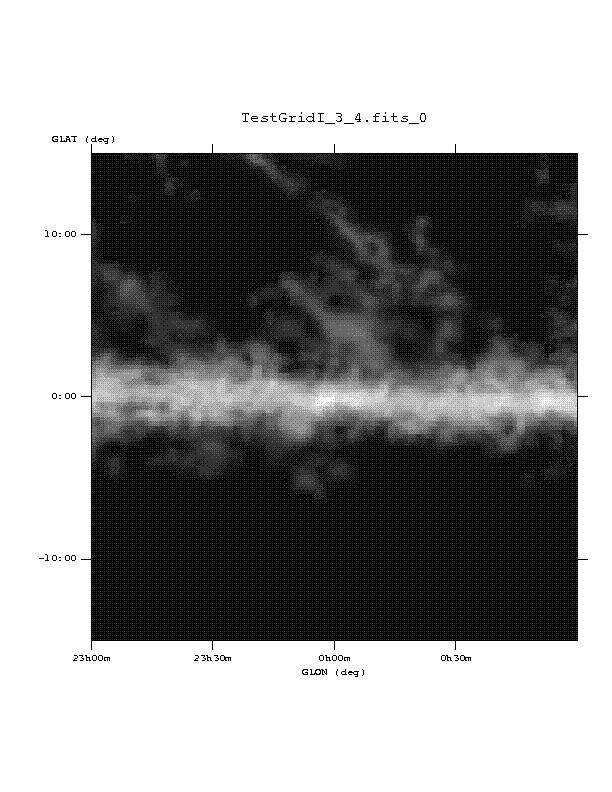
\includegraphics[trim = 50 100 70 100, clip = true, width=0.45\textwidth]{figs/Template_maps/Template4_Ebin01}
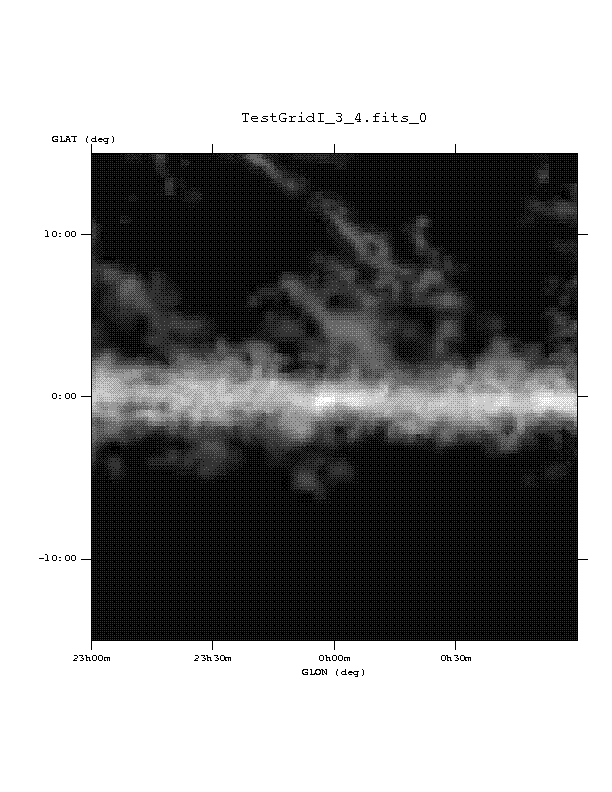
\includegraphics[trim = 50 100 70 100, clip = true, width=0.45\textwidth]{figs/Template_maps/Template4_Ebin71}
\caption{Template 4 flux maps for the first (left) and last (right) energy bin. The flux range is flux = $[-1.43 \cdot 10^{-8}, 1.34 \cdot 10^{-5}]$ (flux = $[-3.66 \cdot 10^{-20}, 2.96 \cdot 10^{-17}]$) in the first (last) energy bin.}
\end{figure}
\begin{figure}
\centering
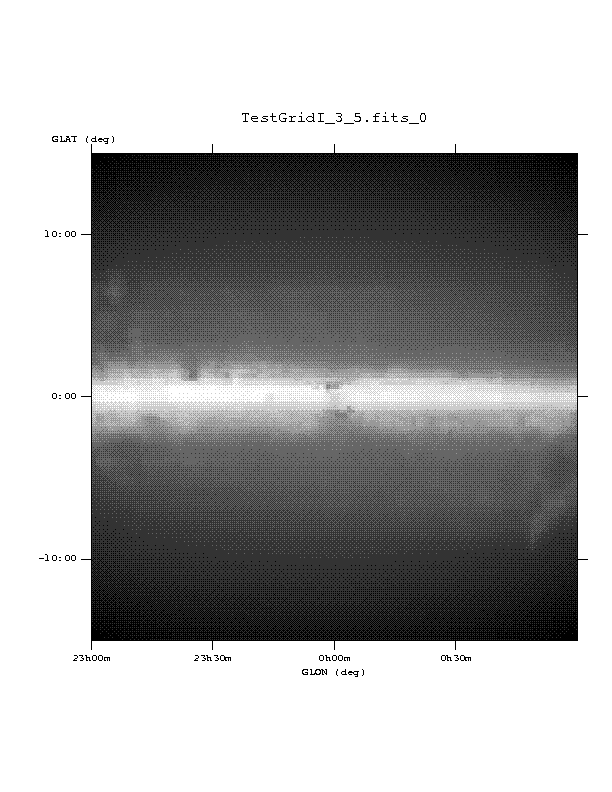
\includegraphics[trim = 50 100 70 100, clip = true, width=0.45\textwidth]{figs/Template_maps/Template5_Ebin01}
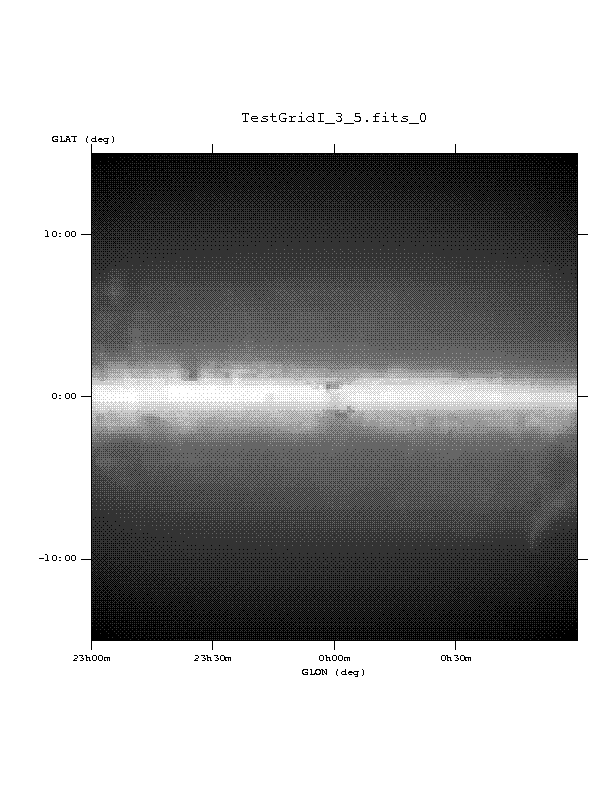
\includegraphics[trim = 50 100 70 100, clip = true, width=0.45\textwidth]{figs/Template_maps/Template5_Ebin71}
\caption{Template 5 flux maps for the first (left) and last (right) energy bin. The flux range is flux = $[1.01 \cdot 10^{-8}, 2.08 \cdot 10^{-6}]$ (flux = $[8.43 \cdot 10^{-19}, 2.15 \cdot 10^{-16}]$) in the first (last) energy bin.}
\end{figure}
\begin{figure}
\centering
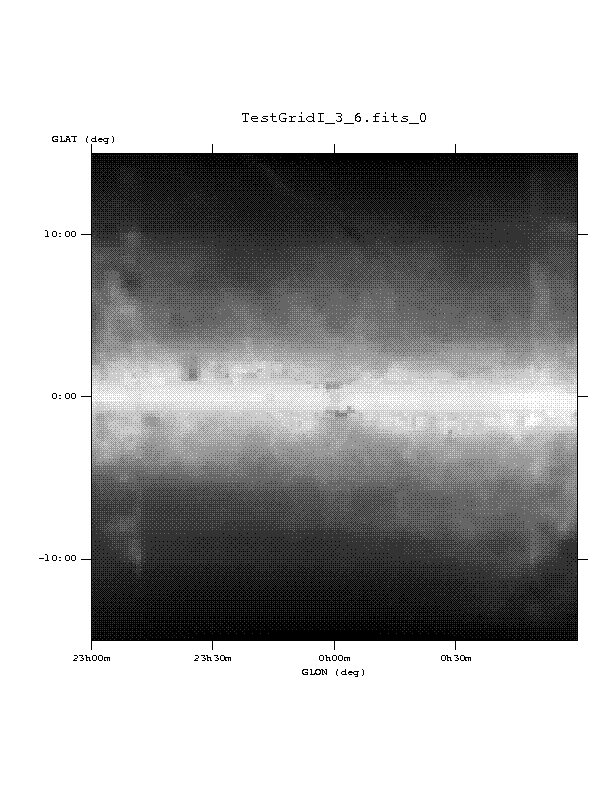
\includegraphics[trim = 50 100 70 100, clip = true, width=0.45\textwidth]{figs/Template_maps/Template6_Ebin01}
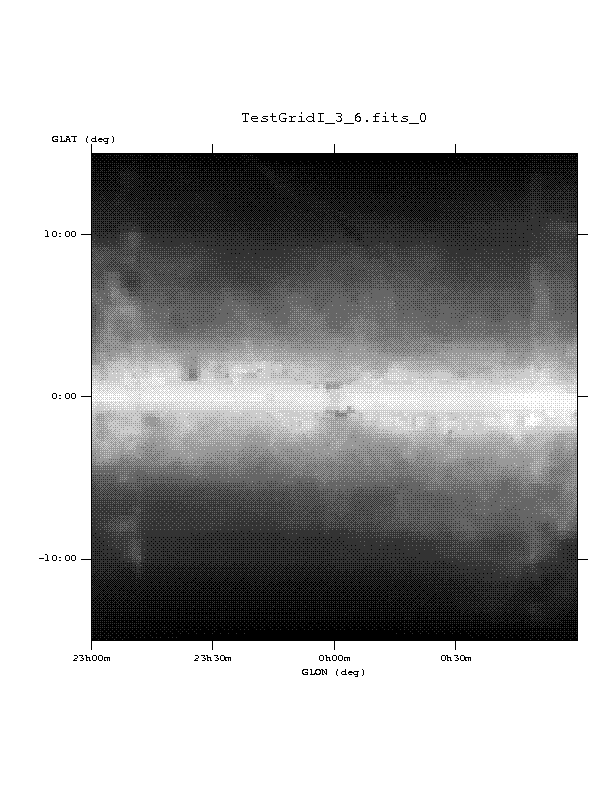
\includegraphics[trim = 50 100 70 100, clip = true, width=0.45\textwidth]{figs/Template_maps/Template6_Ebin71}
\caption{Template 6 flux maps for the first (left) and last (right) energy bin. The flux range is flux = $[1.13 \cdot 10^{-8}, 2.13 \cdot 10^{-6}]$ (flux = $[1.08 \cdot 10^{-18}, 2.42 \cdot 10^{-16}]$) in the first (last) energy bin.}
\end{figure}
\begin{figure}
\centering
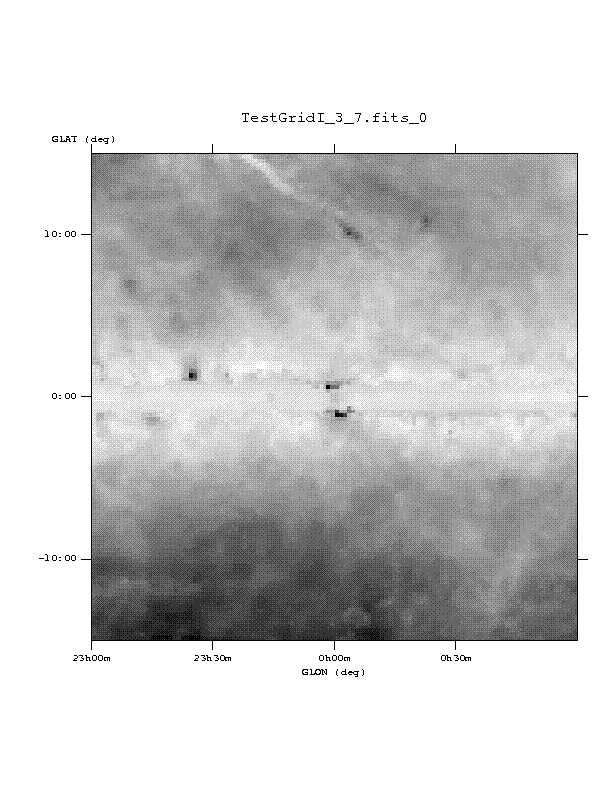
\includegraphics[trim = 50 100 70 100, clip = true, width=0.45\textwidth]{figs/Template_maps/Template7_Ebin01}
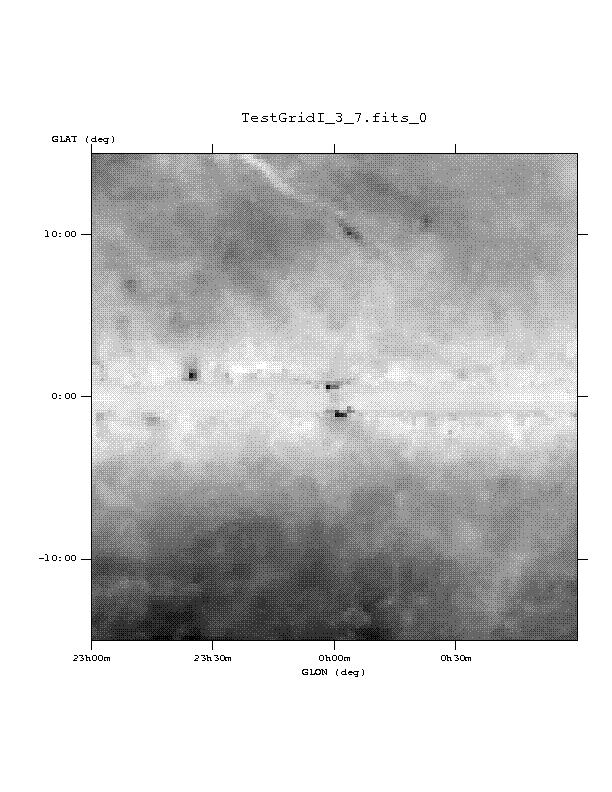
\includegraphics[trim = 50 100 70 100, clip = true, width=0.45\textwidth]{figs/Template_maps/Template7_Ebin71}
\caption{Template 7 flux maps for the first (left) and last (right) energy bin. The flux range is flux =$[1.02 \cdot 10^{-7}, 3.67 \cdot 10^{-6}]$ (flux = $[1.07 \cdot 10^{-17}, 4.04 \cdot 10^{-16}]$) in the first (last) energy bin.}
\end{figure}
\begin{figure}
\centering
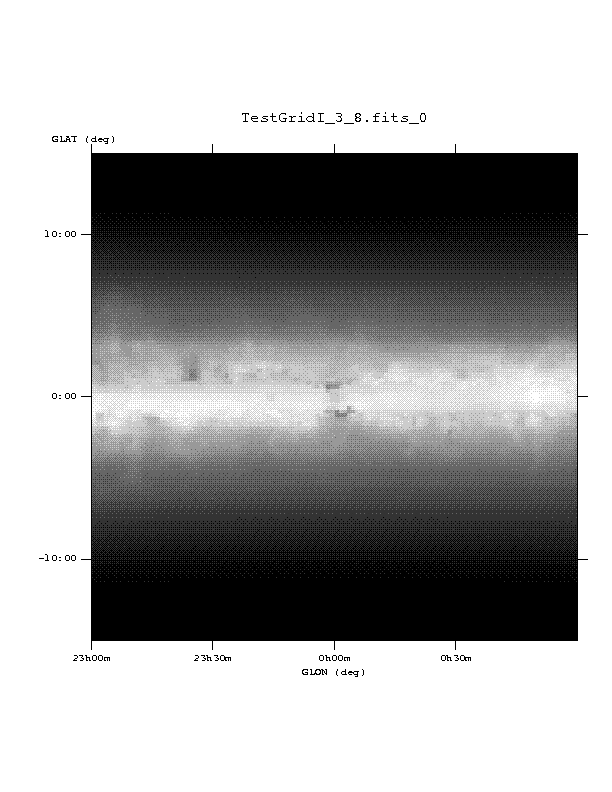
\includegraphics[trim = 50 100 70 100, clip = true, width=0.45\textwidth]{figs/Template_maps/Template8_Ebin01}
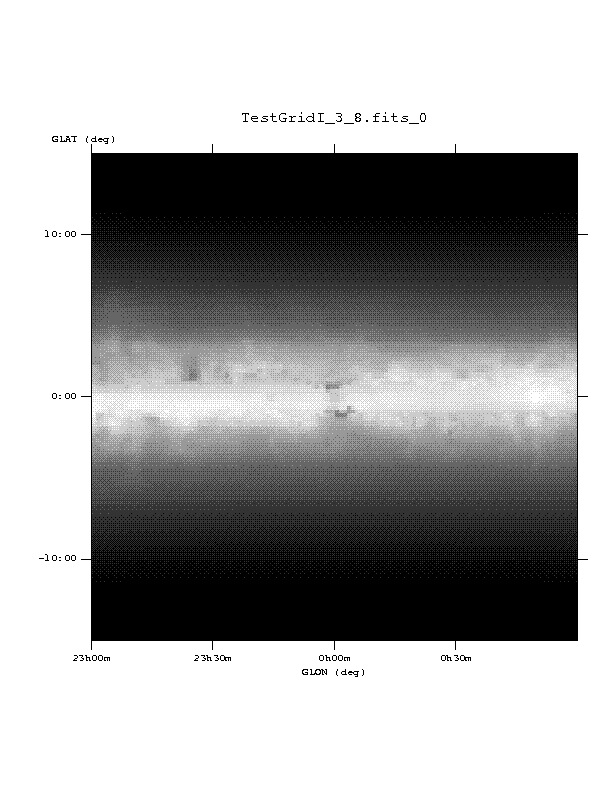
\includegraphics[trim = 50 100 70 100, clip = true, width=0.45\textwidth]{figs/Template_maps/Template8_Ebin71}
\caption{Template 8 flux maps for the first (left) and last (right) energy bin. The flux range is flux = $[-2.04 \cdot 10^{-15}, 2.00 \cdot 10^{-7}]$ (flux = $[-1.49 \cdot 10^{-25}, 1.68 \cdot 10^{-17}]$) in the first (last) energy bin.}
\end{figure}
\begin{figure}
\centering
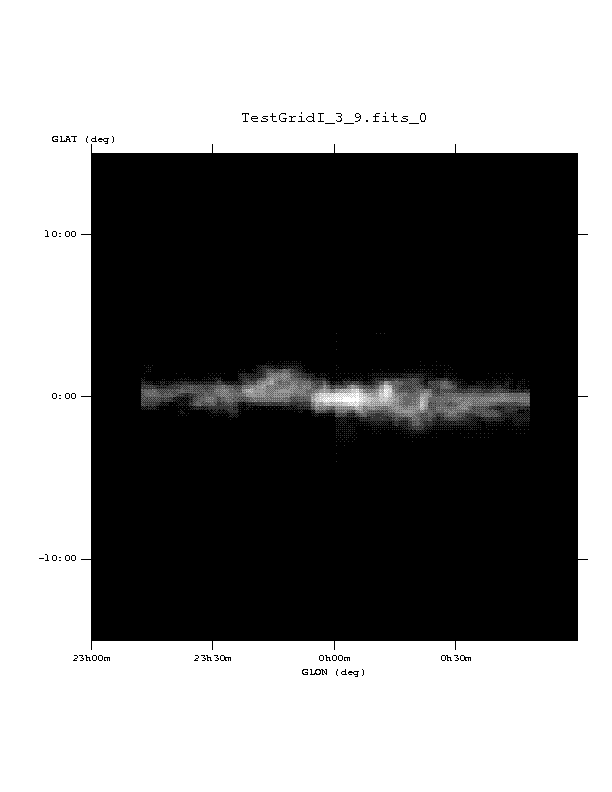
\includegraphics[trim = 50 100 70 100, clip = true, width=0.45\textwidth]{figs/Template_maps/Template9_Ebin01}
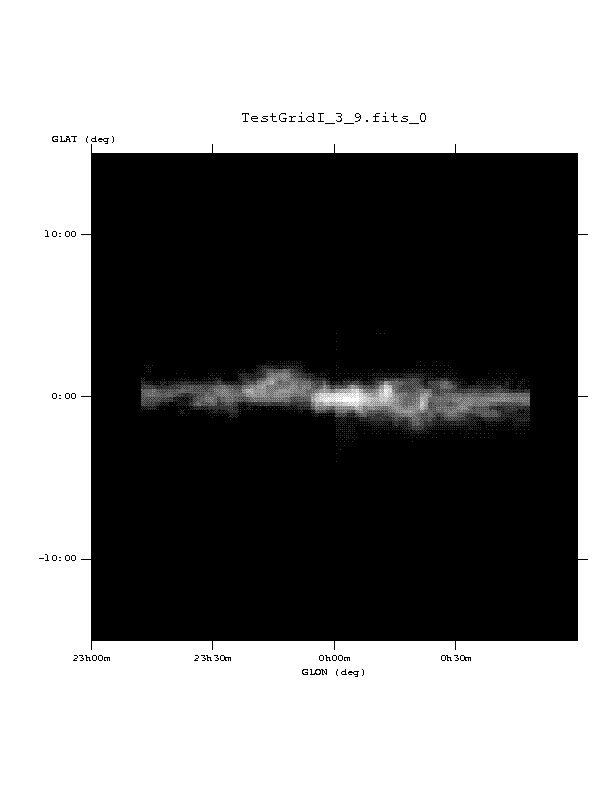
\includegraphics[trim = 50 100 70 100, clip = true, width=0.45\textwidth]{figs/Template_maps/Template9_Ebin71}
\caption{Template 9 flux maps for the first (left) and last (right) energy bin. The flux range is flux = $[-2.12 \cdot 10^{-8}, 1.4 \cdot 10^{-4}]$ (flux = $[-2.10 \cdot 10^{-18}, 1.28 \cdot 10^{-14}]$) in the first (last) energy bin.}
\end{figure}
\begin{figure}
\centering
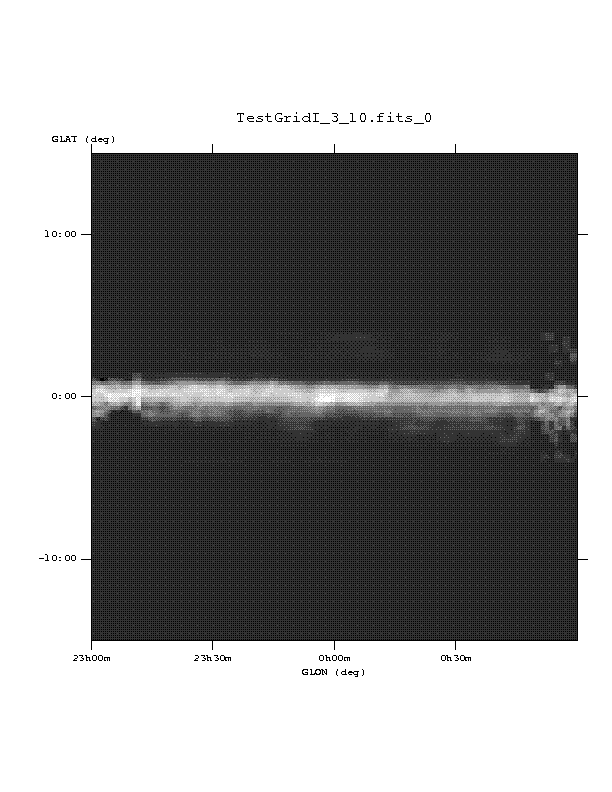
\includegraphics[trim = 50 100 70 100, clip = true, width=0.45\textwidth]{figs/Template_maps/Template10_Ebin01}
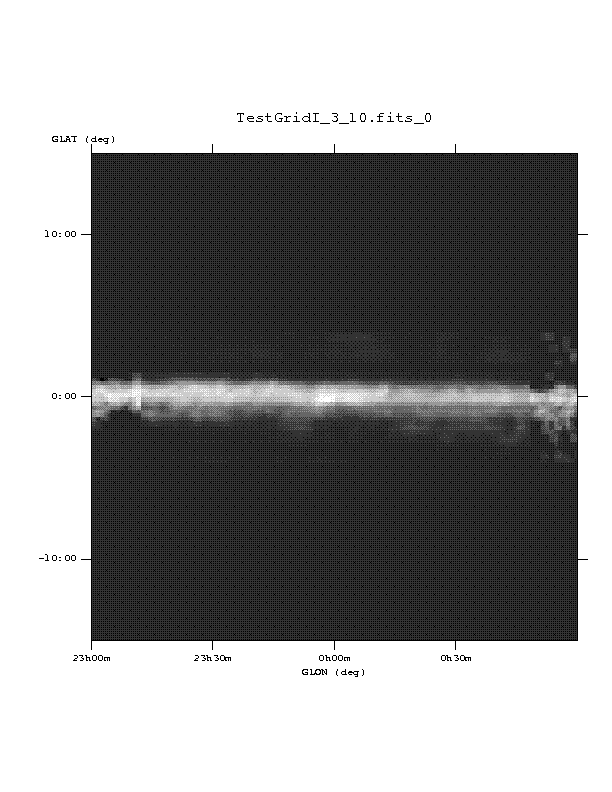
\includegraphics[trim = 50 100 70 100, clip = true, width=0.45\textwidth]{figs/Template_maps/Template10_Ebin71}
\caption{Template 10 flux maps for the first (left) and last (right) energy bin. The flux range is flux = $[-4.53 \cdot 10^{-8}, 8.38 \cdot 10^{-6}]$ (flux = $[-4.74 \cdot 10^{-18}, 8.95 \cdot 10^{-16}]$) in the first (last) energy bin.}
\end{figure}
\begin{figure}
\centering
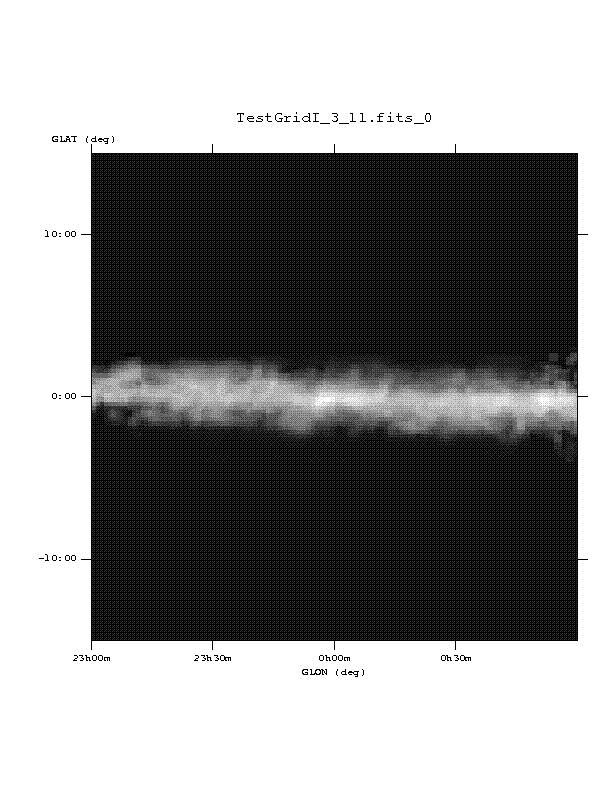
\includegraphics[trim = 50 100 70 100, clip = true, width=0.45\textwidth]{figs/Template_maps/Template11_Ebin01}
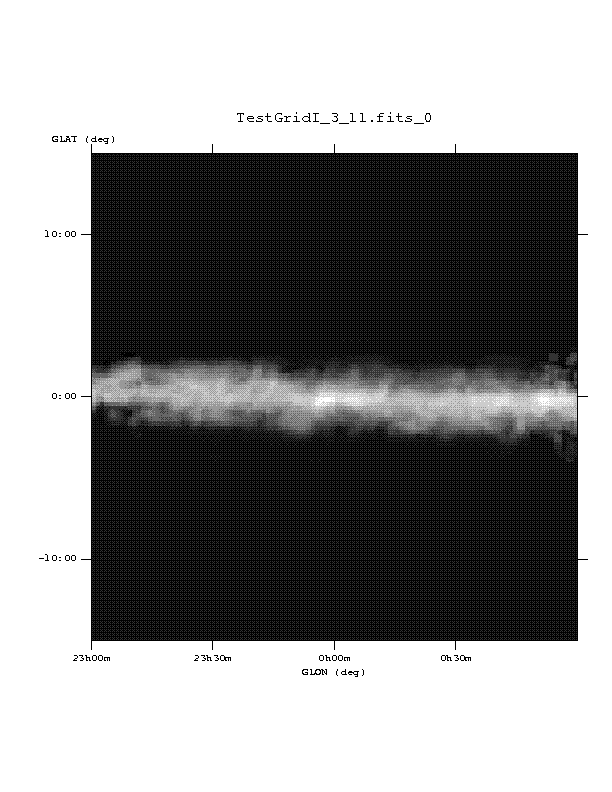
\includegraphics[trim = 50 100 70 100, clip = true, width=0.45\textwidth]{figs/Template_maps/Template11_Ebin71}
\caption{Template 11 flux maps for the first (left) and last (right) energy bin. The flux range is flux = $[-2.81 \cdot 10^{-8}, 1.58 \cdot 10^{-5}]$ (flux = $[-3.16 \cdot 10^{-18}, 1.80 \cdot 10^{-15}]$) in the first (last) energy bin.}
\end{figure}
\begin{figure}
\centering
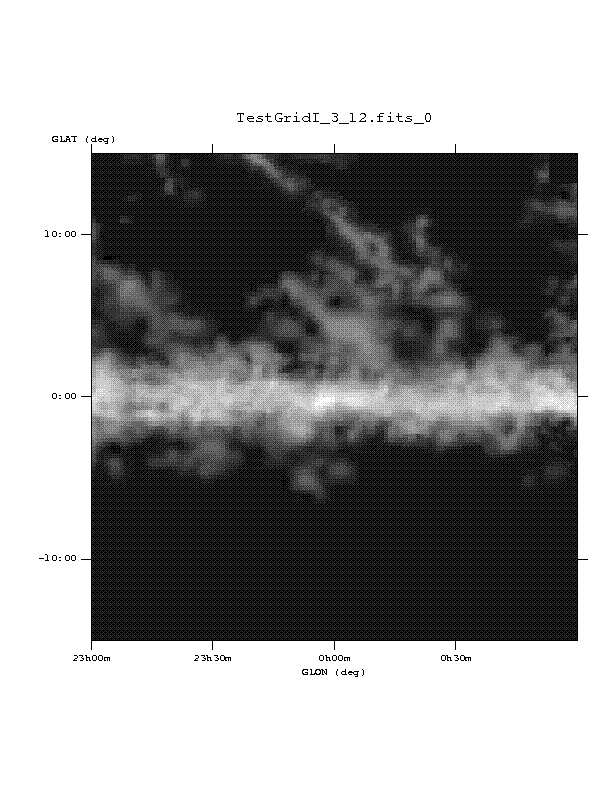
\includegraphics[trim = 50 100 70 100, clip = true, width=0.45\textwidth]{figs/Template_maps/Template12_Ebin01}
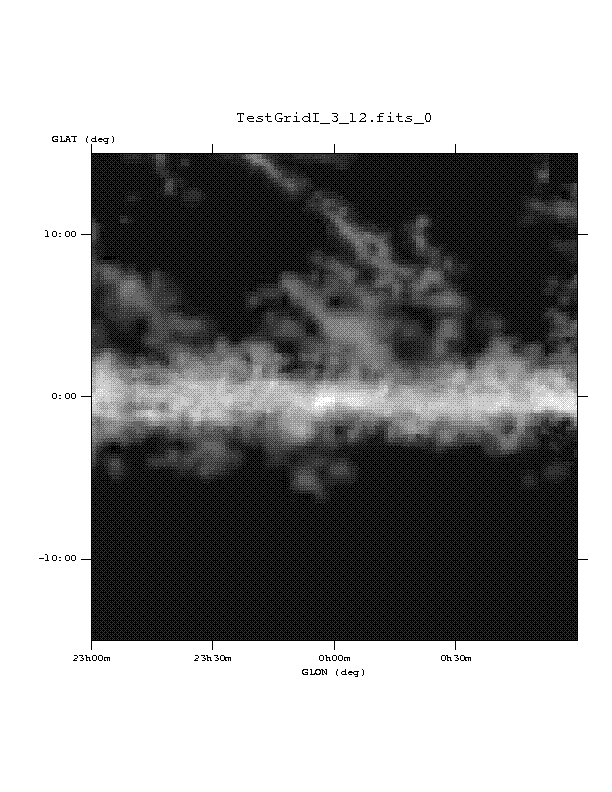
\includegraphics[trim = 50 100 70 100, clip = true, width=0.45\textwidth]{figs/Template_maps/Template12_Ebin71}
\caption{Template 12 flux maps for the first (left) and last (right) energy bin. The flux range is flux = $[-3.59 \cdot 10^{-8}, 1.53 \cdot 10^{-5}]$ (flux = $[-3.75 \cdot 10^{-18}, 1.73 \cdot 10^{-15}]$) in the first (last) energy bin.}
\end{figure}
\begin{figure}
\centering
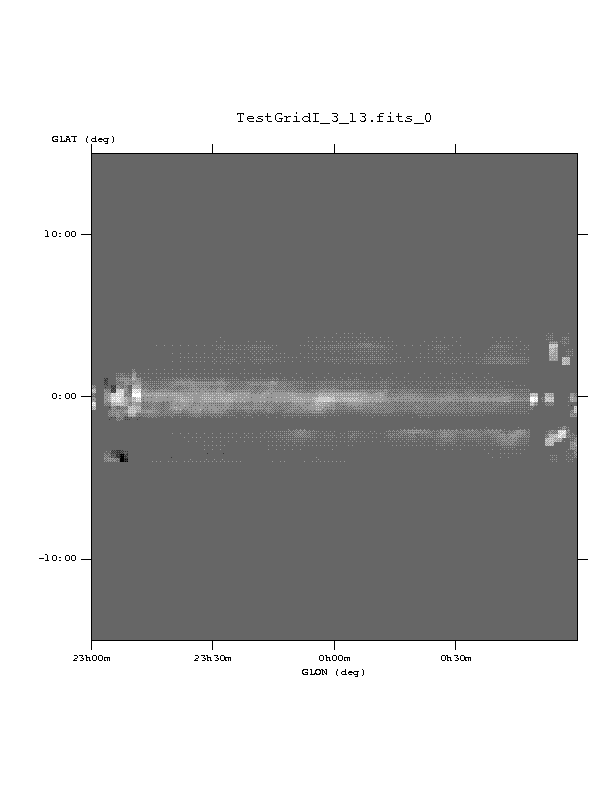
\includegraphics[trim = 50 100 70 100, clip = true, width=0.45\textwidth]{figs/Template_maps/Template13_Ebin01}
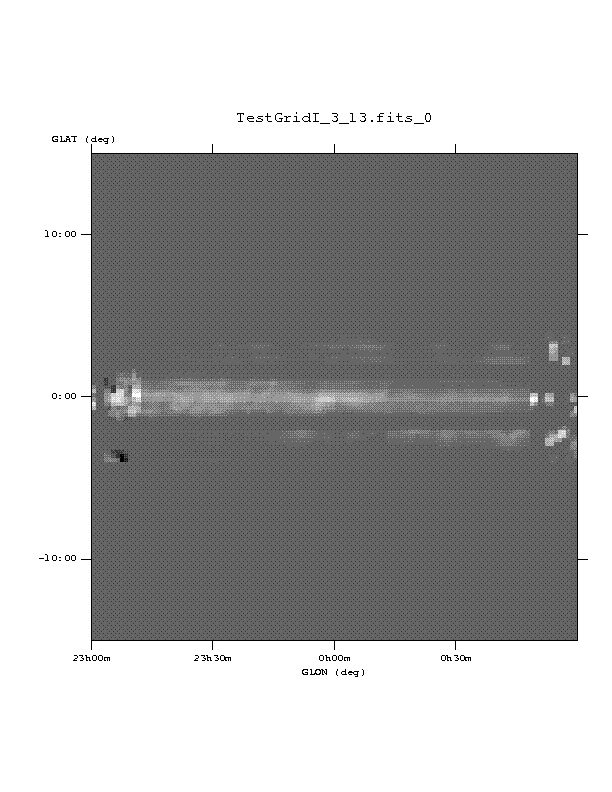
\includegraphics[trim = 50 100 70 100, clip = true, width=0.45\textwidth]{figs/Template_maps/Template13_Ebin71}
\caption{Template 13 flux maps for the first (left) and last (right) energy bin. The flux range is flux = $[-1.41 \cdot 10^{-9}, 4.22 \cdot 10^{-8}]$ (flux = $[-1.10 \cdot 10^{-19}, 3.80 \cdot 10^{-18}]$) in the first (last) energy bin.}
\label{TM13}
\end{figure}
The minimum and maximum flux values corresponding to each template map are given in the caption. By comparing these numbers the contributions of different templates to the total flux can be estimated.


The BG parameters, their parameter type and their prior ranges are given in table \ref{BG_params}. Template parameters are classified according to their rescaling properties. Linear template parameters rescale one or more of the templates in a linear fashion. Special parameters are parameters with more complicated scaling properties. We deal with one grid parameter, six linear parameters and four special (i.e.\ nonlinear) parameters.  The nonlinear parameters are the CR proton and electron spectral indices and source distribution parameters $\alpha$ and $\beta$.  The full set of parameters is given in Table \ref{BG_params}.

\begin{table*}[htbp]
\centering
\fontsize{9}{9}\selectfont
\begin{tabular}{|c|c|c|}
\hline
Parameter & Parameter Type & Prior Range \\
\hline
\hline 
$T_S$($x_S$) & Grid & [100,100000]([-69.9,-34.8]) \\
\hline
$X_{CO}(1)$ & Template (Linear) & [0.1,5.0] \\
\hline
$X_{CO}(2)$ & Template (Linear) & [0.1,5.0] \\
\hline
$X_{CO}(3)$ & Template (Linear) & [0.1,5.0] \\
\hline
index(e) & Template (Special) & [-0.3,0.3] \\
\hline
norm(e) & Template (Linear) & [0.1,10.0] \\
\hline
index(p) & Template (Special) & [-0.3,0.3] \\
\hline
norm(p) & Template (Linear) & [0.1,10.0] \\
\hline
$\alpha$ & Template (Special) & [1.0,5.0] \\
\hline
$\beta$ & Template (Special) & [3.0,10.0] \\
\hline
norm(bubbles) & Template (linear) & [0.1,10.0] \\
\hline
\end{tabular}
\caption{\fontsize{9}{9}\selectfont  Background parameters their parameter type (grid or template; if template linear or special rescaling) and their prior ranges.} \label{BG_params}
\end{table*}

\subsection{Point source fitting methodology}

\subsubsection{Spectral model}

There are different spectra one can use (straight power law, log parabola, exponential cutoff power law). To be able to fit every source at least as well as in the official Fermi point source catalogue, we decided to use a combination of these possible spectra.  This combination is a log parabola with an exponential cutoff:
\begin{equation*}
\frac{\textnormal{d}N}{\textnormal{d}E} = N_0 \left( \frac{E}{E_0} \right)^{-\left[\alpha + \beta \textnormal{log}(E/E_0)\right]} e^{-(E-E_0)/E_\mathrm{c}}.
\end{equation*}
This results in a set of five parameters for the spectrum of a point source $\Theta_\mathrm{spec} = \{ N_0,E_0,E_c,\alpha,\beta\}$, plus two for the position of the source on the sky $\Theta_\mathrm{pos} = l, b$.

\subsubsection{Source identification}

In order to identify the point sources we use Bayesian object detection, following Feroz \& Hobson (2008). During the analysis it is assumed that only one point source is present in some background noise, so that we only have to scan over the parameters for a single point source (+ background parameters). The posterior distribution found by MultiNest has several peaks, each (potentially) corresponding to a different point source. By evaluating the local Bayesian evidence of these peaks and comparing them to the global null evidence (the evidence assuming that there is no point source in the image) one can determine if the peak in the posterior does indeed correspond to a point source. That is, we use Bayesian model selection to distinguish between
\begin{itemize}
\item $H_0$: the detected object is fake (amplitude  = 0, or alternatively amplitude < $A_{lim}$)
\item $H_1$: the detected object is real (amplitude > 0, or alternatively amplitude > $A_{lim}$).
\end{itemize}

This method was shown to work for signal-to-noise ratios of 0.5 - 1.0.  

Note that this approach is known to not work well for separating out two objects that lie very close together and have very different amplitudes.  The other problems when applying this approach to the Fermi GC analysis is that by assuming that only one point source is present in the ROI one will automatically overestimate the background (which then receives contributions from all other point sources), and at the same time underestimate the point source amplitude. Scanning of complicated models in this way also takes forever, so there is no way this technique can be used to do detailed background or spectral fits.  We therefore apply it only for determining the existence and approximate location of point sources.  We then turn to differential evolution for carrying out detailed fits and profile likelihoods of the spectral parameters of sources identified with Bayesian object detection, and for determining background and DM parameters.

\subsubsection{Point source parameter estimation}

To fit the parameters of point sources after identifying them with MultiNest, we use a genetic-inspired optimisation algorithm, Differential Evolution, as implemented in the code \textsc{Diver}. In a nutshell, it makes a population of individual parameter points, treats them as vectors within the parameter space, and evolves the population towards better fits by carrying out various vector addition, subtraction and replacement operations on the different vector components of different individuals.  This evolutionary process includes a mutation element, and depends on the whole population, allowing the fittest individuals to evolve towards the parameter combination returning the highest likelihood. The idea is to find the point sources' positions with MultiNest, and then fit all the parameters of those sources with Diver, hoping for a better accuracy.  This seems to work pretty well from the tests that we have done so far (details below).

\subsubsection{Unified fit strategy}
\label{UFS}

Our overall iterative fitting method is thus as follows:

\begin{enumerate}
\item Background (simple 3D parameterisation: $T_S$, $X_{\rm CO, global}$, globalnorm(p)) and point source fit (3 parameters ($l$,$b$,$N_0$) high energy bins only).  Posterior scan (MultiNest), 6D.
\item Background (simple 3D parameterisation) fit for null evidence.  Posterior scan (MultiNest), 3D.
\item Background (full 11D parameterisation) and point source fit (5 parameters, high and low E bins, with positions fixed to best-fit values from step 1), with Known Point Source Index discrete parameter, iteratively setting parameters of point sources *not* corresponding to the value of the index parameter to their current best-fit values as the scan progresses and those best-fit values improve.  Gradually improves the fits of the known point sources.  Likelihood-only scan (Diver), 17D.
\item Repeat Steps 1--3, with found PS and 8 non-simple BG values fixed to their best fit values from Step 3 when repeating Step 1.  Repeat until all point sources seem to have been found, i.e.\ no more pass the null evidence cut.
\item Repeat steps 1 and 2 also including low energy bins, to make sure we didn't miss any PS that don't show up in the high E bins.  If we did miss any, run them through steps 3 and 4 to get their parameters.
\item Repeat step 3 one last time, including all PS found to this point, and also allowing their positions to vary.  The point sources should start the fit with their current best-fit values.
\item Calculate the local evidence for each PS (i.e.\ find the difference in the evidence found when including all PS, and when excluding a certain PS from the model). Discard the ones that don't pass the evidence threshold (\ps{this threshold still to be defined}).
\item Fix the point source parameters to the best fit values.  Background (full 11D parameterisation) and DM fit (full 15D parameterisation).  Likelihood-only scan (Diver), 26D.

\end{enumerate}

\subsubsection{Results of point-source tests}

To test the ability of our unified fit strategy (\ref{UFS}) to accurately recover point sources, we implemented a full simulation facility in \textsc{DMBayes} a la \textit{gtobssim}, as well as routines to access the 2-year LAT point-source catalogue as a source of mock point sources.

\subsubsection*{Steps 1-2}

\textbf{Test 1} (Charlotte): Results for a point source identification scan in a fixed background are shown in Fig.~\ref{3D_PS_results}. Parameters scanned over are the two position parameters and the amplitude, i.e.\ the spectrum of the PS is fixed. The scan includes all 46 PS extracted from the catalogue (corresponding to roughly $4\sigma$ sources). Point sources marked in blue are found by the scan and their parameters are correctly identified (i.e.\ the amplitude is off by at most 0.1 log units). Pink sources are found by the scan, but their best-fit amplitude is different from their true amplitude. For all of these mismatched PS the difference between true and best-fit amplitude is $\Delta$ log$(N_0) \leq 1.0$. Point sources shown in red were not found by the scan. Note that all of the missed PS correspond to a relatively low amplitude log$(N_0) \leq -12.0$.  Results are quite encouraging, but unsurprisingly the Galactic Centre region is very challenging.  Iterative application of this technique after fitting the parameters of the found sources should clear up most of the poor fits and missing sources.

\begin{figure}[h]
\centering
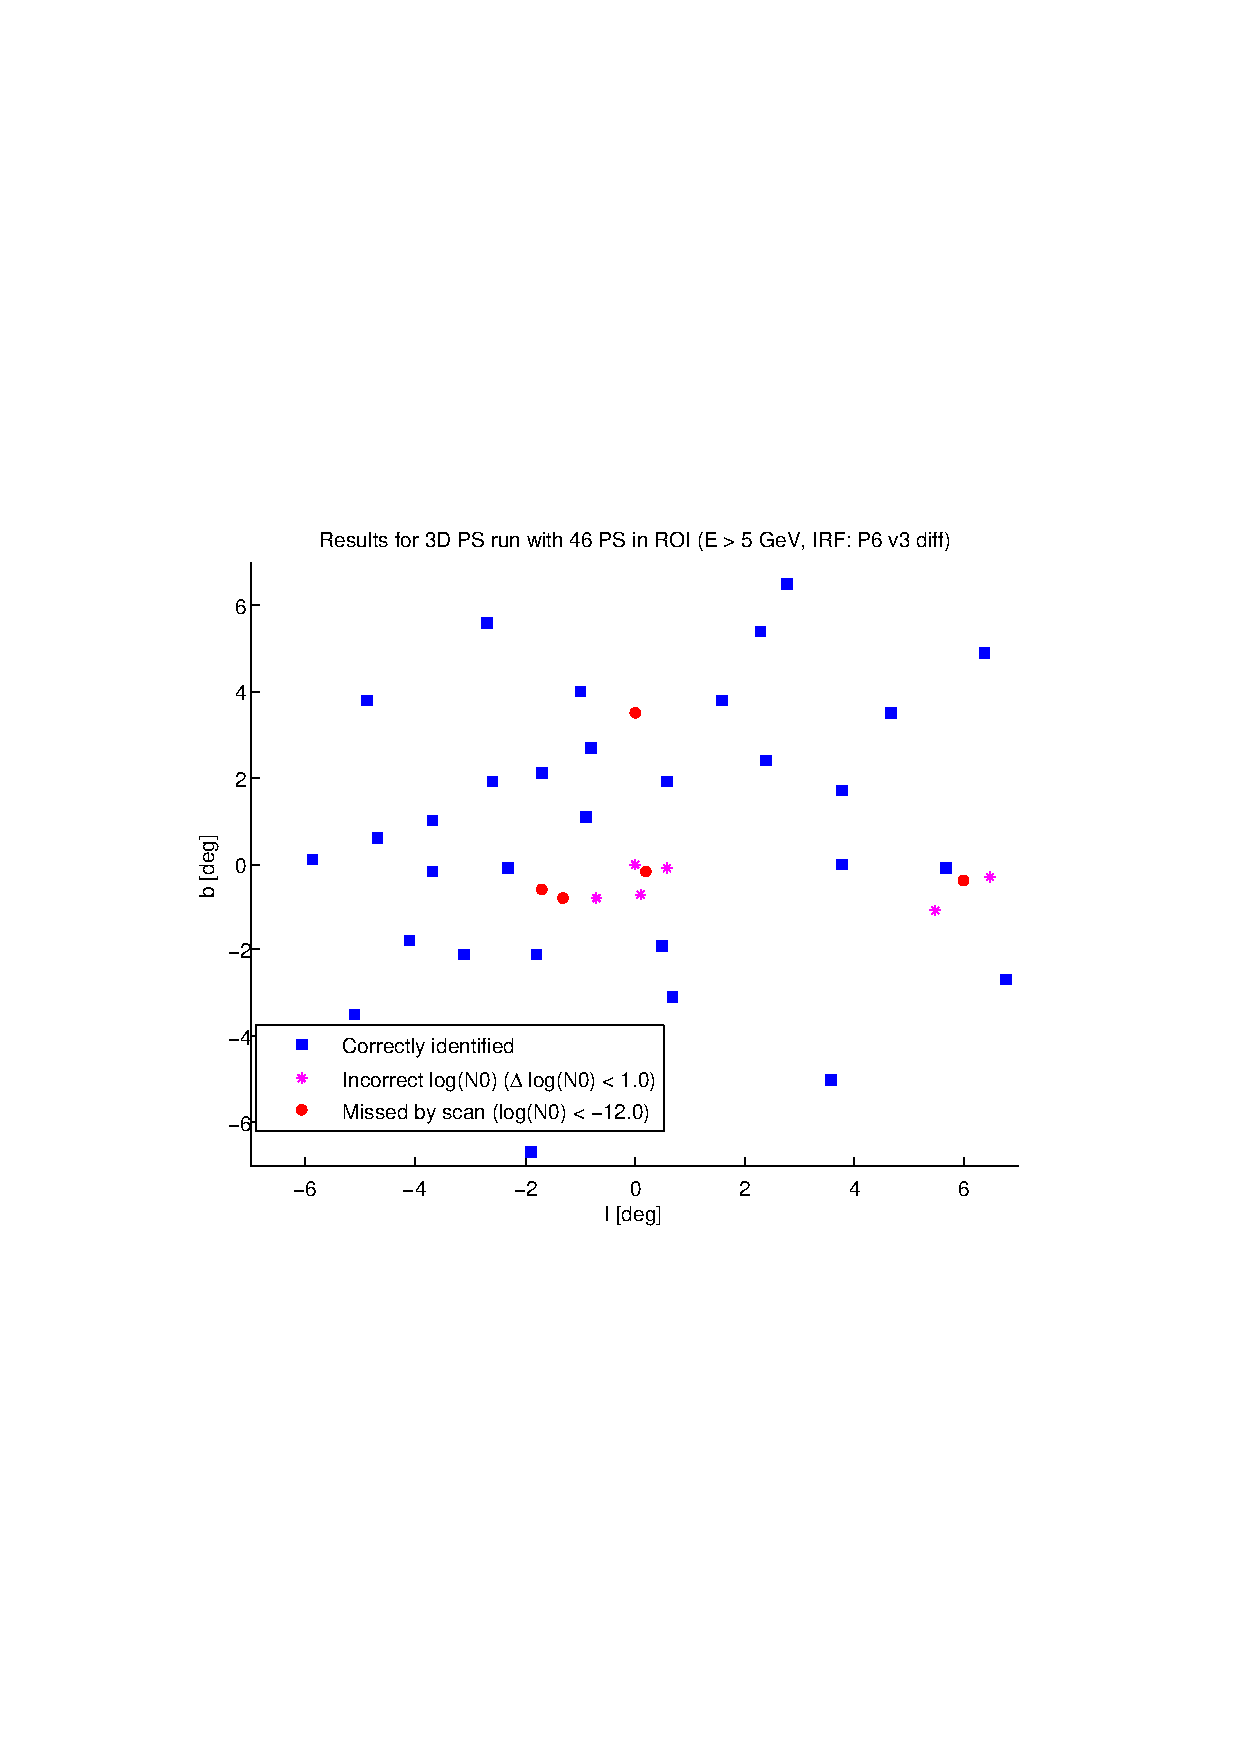
\includegraphics[trim = 90 200 100 230, clip = true,width=0.75\textwidth]{figs/3D_50PS_BG_fix.pdf}
\caption{Results for the identification of PS in a fixed background, scanning only over the two position parameters and the amplitude, and discarding information from the first 9 energy bins.\label{3D_PS_results}}
\end{figure}

\textbf{Test 2} (Anotoine):
\begin{itemize}
\item MultiNest 6D, first run
\item ini file: \verb=46PS_6DMNRunI.ini=\footnote{To remake those runs on the HPC with walltime = 72hrs, one will need to restart and continue, i.e.\ to change the \verb=restart_and_continue= from F to T in this ini file after 72 hrs.}
\item nCdims = 2, nlive = 4000,tol = 0.02,eff = 0.3
\item Null evidence ini file: \verb=MNNullRunI.ini=
\end{itemize}
31 modes were found, of which 4 were discarded by the Null evidence (i.e.\ they have a local evidence strictly lower than the global evidence found in the Null run). Figure \ref{fig:scatterplot46PSMNI} shows $\chi^{2} = - 2Log(Likelihood)$ as a scatterplot in ($l$,$b$) after this run, featuring the true point sources. At this stage, one can see that 9 point sources are missed by the scan, and some that lie close one to each other are not separated out.
\begin{figure}[h]
\centering
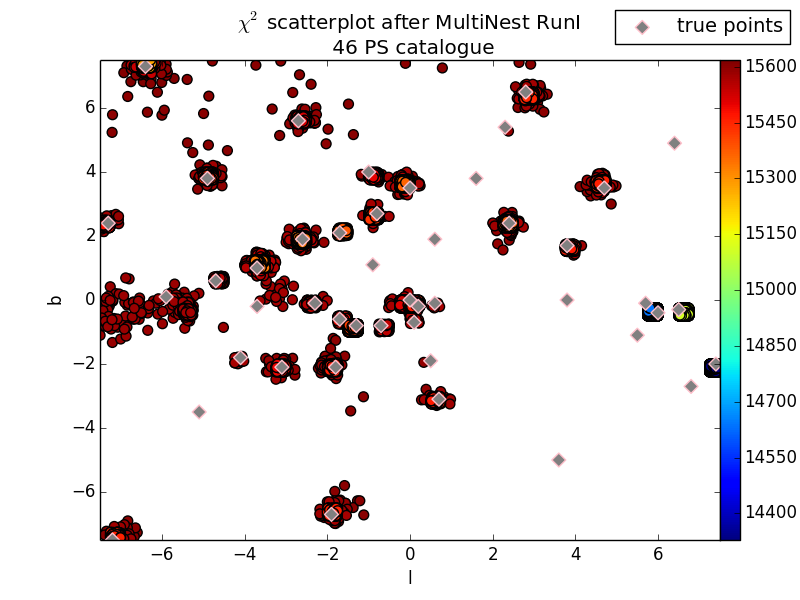
\includegraphics[clip = true,width=0.75\textwidth]{figs/scatplt46PSafterMNRunI.png}
\caption{$\chi^{2}$ scatterplot after MultiNest 1st run for the 46PS with BG\label{fig:scatterplot46PSMNI}}
\end{figure}

\subsubsection*{Step 3}

\textbf{Test 1} (Grace): details not shown -- good fits obtained with up to 10 point sources, bugs encountered thereafter.  Bugs fixed.  Plotting scripts and ini files passed on to Antoine.

\textbf{Test 2} (Antoine): We tested the efficiency of Step 3 with a fake data set generated from the 46 PS from the catalogue, in a set background (3rd grid point, all templates not rescaled, i.e.\ $x_S = -49.6$, $X_{CO, global} = 1$, $norm_e = norm_p = 1$, $index_e = index_p = 0$, $\alpha = 2$, $\beta = 5$). The ini files referred to here can be found in \verb=antoine_for_the_record/46PS/ini_files/= on the svn main directory. 

These tests were Diver 11D runs (3D for the BG, 7D per PS and 1D: PS index). \begin{itemize}
\item ini file: \verb=46PS_11DDiverRunI.ini=
\item follow up file: \verb=27modes_above_nullev.txt=
\end{itemize}
I set \verb=gen_tol_smooth_len= = 300 (=number of generations) in this run to prevent Diver from stopping when the convergence criterion is wrongfully fulfilled\footnote{The convergence criterion is: no improvement in the mean likelihood amongst all subpopulations during \verb=gen_tol_smooth_len=, but if a subpopulation (point source) does not fall into the allowed l,b range, its logLike$\sim \infty$ which numbs the effect of the other subpopulation's improvement. Setting \verb=gen_tol_smooth_len==\verb=maxgen= keeps this criterion from being reached during the whole run.}. \\
One point source never fell in the allowed box in $l,b$ around the position determined from the MultiNest run in Step 1\footnote{This should no longer happen now, as the prior for Diver is no longer `LogZero' everywhere outside the allowed box, but something like logZero*(1+distance from allowed box)}, and the others converged properly (see figures \ref{fig:DiverIBFLike} and \ref{fig:DiverIcgce}).
\begin{figure}[h]
\centering
\includegraphics[clip = true,width=0.75\textwidth]{figs/DiverIBFLike.png}
\caption{Best fit likelihood for Diver first run (Step 3) with 46 PS. The dashed line is meaningless here (does not actually corresponds to the true point value)\label{fig:DiverIBFLike}}
\end{figure}
\begin{figure}[h]
\centering
\includegraphics[clip = true,width=0.75\textwidth]{figs/DiverIcgce.png}
\caption{Convergence Criteria for Diver first run (Step 3) with 46 PS. The weird features before generation 130 are due to points not yet in the allowed l,b range (the missing points are 0., since there is no likelihood change during a period at which all points but one have fallen into the allowed range)\label{fig:DiverIcgce}}
\end{figure}
More plots from this run, including the scatter plots in projections of the parameter space for each point source, are in \verb=for_the_record/figures/DiverI/= (and in \verb=DiverI_extended=, are those plots for a greater value of \verb=maxgen=. They are given for comparison -- the best fits used for the second run of MultiNest are the ones from \verb=DiverI=, and there is no substantial improvement between generation 300 and 400). The results are not fully satisfying: a few point sources are ``well fitted'', but for most of them there is a sizeable discrepancy between the true and best fit values of $\alpha$, $\beta$, $N_0$ and $E_0$: see table \ref{table:DiverI} (probably the plots from the DiverI directory are a bit clearer).  Still, it is only the first iteration of Step 3, and only 27 point sources are fitted to account for a map with 46 at this point, so it would have been surprising to find a perfect fit for those points straight away.

\begin{table}[hbt]
\centering
\begin{tabular}{|c|c|c|c|c|c|c|c|}
\hline
PS & $l$ & $b$ & $N_0$ & $E_0$ & $\alpha$ & $\beta$ & $1.e5/E_C$ \\
\hline
1 & -4.9 (-4.9) & 3.8 (3.8) & -12.9 (-12.3) & 2645 (1894) & 1.11 (2.24) & 0.38 (0.00) & 0.05 (0.00) \\
2 & 5.1 (4.7) & 4.4 (3.5) & -10.4 (-11.4) & 613 (878) & 0.67 (2.43) & 0.71 (0.00) & 268.54 (0.00) \\
3 & -2.5 (-2.7) & 5.5 (5.6) & -12.6 (-11.4) & 718 (730) & 0.09 (2.45) & 0.48 (0.00) & 0.46 (0.00) \\
4 & 2.9 (2.8) & 6.4 (6.5) & -11.8 (-12.0) & 966 (1353) & 1.86 (2.30) & 0.15 (0.00) & 0.01 (0.00) \\
5 & -7.3 (-7.3) & 2.3 (2.4) & -12.7 (-10.8) & 4604 (996) & 2.33 (2.51) & 0.12 (0.25) & 22.08 (0.00) \\
6 & -1.2 (-1.7) & 2.1 (2.1) & -12.7 (-12.3) & 572 (2159) & 1.18 (2.26) & 0.88 (0.00) & 8.99 (0.00) \\
7 & 7.3 (6.5) & 1.7 (-0.3) & -13.2 (-10.4) & 559 (1411) & 2.42 (2.39) & 0.93 (0.35) & 100.72 (0.00) \\
8 & 1.3 (-0.0) & 3.8 (3.5) & -11.6 (-12.0) & 1129 (1633) & 2.10 (2.30) & 0.69 (0.00) & 199.48 (0.00) \\
9 & 7.1 (6.5) & -0.3 (-0.3) & -12.6 (-10.4) & 1815 (1411) & 2.99 (2.39) & 0.00 (0.35) & 135.80 (0.00) \\
10 & 6.5 (5.7) & -0.3 (-0.1) & -11.1 (-11.5) & 3058 (1902) & 2.94 (2.55) & 0.40 (0.44) & 9.61 (0.00) \\
11 & 4.0 (3.8) & 1.6 (1.7) & -11.8 (-11.2) & 2803 (1643) & 1.97 (2.30) & 0.47 (0.37) & 11.55 (0.00) \\
12 & -0.6 (-0.0) & -0.5 (-0.0) & -12.4 (-10.4) & 4874 (1618) & 1.41 (2.34) & 0.00 (0.25) & 69.57 (0.00) \\
13 & -0.2 (-0.0) & -0.5 (-0.0) & -12.1 (-10.4) & 4691 (1618) & 1.01 (2.34) & 0.00 (0.25) & 98.72 (0.00) \\
14 & -0.7 (-0.9) & 1.1 (1.1) & -10.6 (-10.5) & 908 (813) & 0.99 (2.70) & 0.16 (0.68) & 220.09 (0.00) \\
15 & -2.0 (-0.9) & 0.2 (1.1) & -12.0 (-10.5) & 1734 (813) & 0.50 (2.70) & 0.27 (0.68) & 384.45 (0.00) \\
16 & -3.7 (-3.7) & 1.0 (1.0) & -12.0 (-10.6) & 4837 (1302) & 2.99 (1.11) & 0.60 (0.00) & 13.09 (49.50) \\
17 & -2.3 (-2.6) & 1.9 (1.9) & -12.9 (-12.0) & 687 (1913) & 0.34 (2.26) & 0.14 (0.00) & 343.61 (0.00) \\
18 & 2.3 (2.4) & 2.5 (2.4) & -12.6 (-12.1) & 2629 (1832) & 1.81 (2.20) & 0.06 (0.00) & 0.93 (0.00) \\
19 & -1.0 (-0.8) & 2.6 (2.7) & -11.9 (-11.9) & 1365 (1545) & 2.33 (2.39) & 0.00 (0.00) & 0.04 (0.00) \\
20 & -1.6 (-1.7) & 2.1 (2.1) & -12.1 (-12.3) & 1454 (2159) & 1.81 (2.26) & 0.06 (0.00) & 0.91 (0.00) \\
21 & -2.6 (-2.6) & 1.8 (1.9) & -12.3 (-12.0) & 1860 (1913) & 1.54 (2.26) & 0.20 (0.00) & 0.03 (0.00) \\
22 & -3.5 (-2.6) & 1.4 (1.9) & -13.0 (-12.0) & 824 (1913) & 0.73 (2.26) & 0.63 (0.00) & 420.30 (0.00) \\
23 & -0.2 (-1.0) & 3.6 (4.0) & -11.4 (-11.5) & 658 (907) & 1.49 (2.52) & 0.18 (0.00) & 0.01 (0.00) \\
24 & -0.8 (-0.0) & 4.0 (3.5) & -12.3 (-12.0) & 827 (1633) & 0.08 (2.30) & 0.60 (0.00) & 0.04 (0.00) \\
25 & -6.5 (-6.4) & 7.4 (7.3) & -12.5 (-11.5) & 1196 (1043) & 2.10 (2.24) & 0.80 (0.00) & 6.45 (0.00) \\
26 & -6.4 (-6.4) & 7.3 (7.3) & -13.2 (-11.5) & 6097 (1043) & 1.89 (2.24) & 0.09 (0.00) & 1.77 (0.00) \\
\hline
\end{tabular}
\caption{best fit (true value) for each point source parameter after Diver first run.}\label{table:DiverI}
\end{table}

\subsubsection*{Step 4 (repeat of 1+2)}

\begin{itemize}
\item MultiNest 6D, RunII
\item ini file: \verb=46PS_6DMNRunII.ini=
\item Null evidence: \verb=MNNullRunII.ini=
\item nCdims = 2, nlive = 3000, tol = 0.01, eff = 0.3
\end{itemize}
The 26 point sources fitted by \textsc{Diver} in the previous step are now added to the model\footnote{This is currently 
hardcoded in calclike.f90 - search '!AR' comments to find where exactly. \ps{I will implement new code that allows this 
to be automated from step to step.}}, to find the left point sources on top. So far (the run is not finished yet), MultiNest 
has found 14 modes, but unfortunately it does not seem to be any of the ones missed in the first run, but either points 
that lie close to one previously found, or just ``another finding of one same point source'' (if, for example, its amplitude 
has been underestimated in steps 1 to 3) : see figure \ref{fig:scatterplot46PSMNII}. We can hope to find the rest of the 
point sources in further iterations of steps 1-3 (with more live points/lower tolerance?), or perhaps when adding the low 
energy bins.
\begin{figure}[h]
\centering
\includegraphics[clip = true,width=0.75\textwidth]{figs/scatplt46PSafterMNRunII.png}
\caption{$\chi^{2}$ scatterplot after MultiNest 2nd run for the 46PS with BG\label{fig:scatterplot46PSMNII}}
\end{figure}
\FloatBarrier

\subsubsection*{Step 5 (test 1 to 4)}
(Andrea) The MultiNest run found 28 point sources, only 17 of which had Local Evidence strictly higher than the Global 
Evidence in the null hypothesis (3D MultiNest scan). Those point sources are shown in the Fig.~\ref{fig:17MN}. The adopted parameters are the following:
\begin{itemize} 
\item nCdims=2 (corresponding to $l,b$)
\item live=3000
\item eff=0.3
\item tol=0.01
\end{itemize}
\begin{figure}[h]
\centering
\includegraphics[clip = true,width=1\textwidth]{figs/MNmodes_46TruePS.png}
\caption{$\chi^{2}$ scatterplot of 17PS found after MultiNest 1st run against the 46 true PS}
\label{fig:17MN}
\end{figure}
The 17 MultiNest-found point sources have then been input into Diver, which returned their best-fit parameters, separating 
the 1/3 brightest of these in a different output file to be then used as model input in the next iteration of MultiNest. The result 
of this run, for all 17 point sources, is shown in Fig.~\ref{fig:6Diver}. This figure clearly displays the presence of an issue with Diver as 
some MultiNest (reasonably well) fit point sources' position are best-fit far away from the corresponding true point source position. 
The probable underlying explanation is an attempt by Diver to simultaneously fit two nearby point sources with a single one accounting 
for the emission of both. This problem can be due to the broadening of the IRF at low energies, leading to the overlap of two 
neighbouring point sources at the low energy bins which, differently from MultiNest, are examined by Diver. \newline
\begin{figure}[h]
\centering
\includegraphics[clip = true,width=1\textwidth]{figs/MultiNest_Diver.png}
\caption{$\chi^{2}$ scatterplot after MultiNest 1st run for the 46PS with simple (3D) BG}
\label{fig:6Diver}
\end{figure}
This issue has urged the following modification in the UFS: Dicrease the dimensionality of the parameter space scanned for each 
PS by Diver from 19D to 17D, where the position of each PS is to be kept fixed at the MultiNest-found values. This will avoid the point 
sources from being shifted away from the true PS position while still providing an improved spectral fit. At the final iteration of 
MultiNest - i.e. when no more found point source passes the Global Null Evidence - Diver is run one final time letting the full 
19D parameter space of all point sources to be examined.

\section{To do}

\subsection{Things missing from these notes}
\begin{itemize}
\item Comment about treatment of extended sources in our ROI (such sources do show up in 2FGL catalogue)
\item Add some information on DM profile parameters (3 generalised NFW, 1 local DM density)  
\item Add brief results of the BG reconstructions Charlotte did
\item Add brief results of the PS reconstructions Grace did
\end{itemize}

\subsection{Remaining analysis design issues}
\begin{itemize}
\item What is a reasonable value to use in Step 6?
\item Should we use front-converting events or both front- and back-converting events? (Use one at low and one at high energies?  This would slow down the runs, since we have to store twice as many files in memory.)
\item Pass 8?
\end{itemize}

\subsection{Outstanding code implementations}
\begin{itemize}
\item Re-jig code to seamlessly operate any of the steps in Sec \ref{UFS}, without recoding each time (Pat)
\item Discard faintest 2/3 of point sources found in each iteration of Step 1 before moving on to Step 3 (Pat)
\item Add Fermi bubble template (+obtain from Meng Su / Christoph W)
\item Set the EGBG normalisation in the diffuse model database index file
\item Decide on final resolution of undefined pixel error in BG maps Gulli sent
\item Get new simulated data files with the correct resolution and starting at 300\ MeV (instead of 100\ MeV). \ps{Not sure if this actually still needs doing?}
\item Analyse 2 or more years of real Fermi data
\end{itemize}

\subsection{Tests still to be completed}

Definitely to be done:
\begin{itemize}
\item Test Steps 1-4 fully run through to convergence (current tests only include 3D BG in Step 3, lack a bubble template, do not discard the fainter 2/3 of sources after Step 1, and are not yet converged wrt Step 4.)
\item Test Step 5
\item Test run of a BG + DM reconstruction (Step 7)
\item Test run of a BG + DM + PS reconstruction (Step 7)
\end{itemize}

Previously planned \ps{and not sure if we need to actually do or not}:
\begin{itemize}
\item Test the reconstruction procedure on the point sources map from Simona \cs{Roberto, are we still planning to do this? Have you heard from Simona about this?}
\item Test reconstructions using DM profile nuisance params
\item Test the prior on the annihilation cross-section in a DM only scan using the mapcubes Tesla sent
\end{itemize}

\end{document}
